%DIF 1c1
%DIF LATEXDIFF DIFFERENCE FILE
%DIF DEL /Users/nadeaus/Documents/Repos/poumm-gwas/manuscript/mbe-submission/hiv-gwas.tex                     Thu Jun 23 14:18:04 2022
%DIF ADD /Users/nadeaus/Documents/Repos/poumm-gwas/manuscript/mbe-reviews/re-submitted/hiv-gwas-for-dff.tex   Thu Jun 23 14:18:59 2022
%DIF < \documentclass[12pt]{article}
%DIF -------
\documentclass[11pt]{article} %DIF > 
%DIF -------
\usepackage[margin=1in]{geometry}
%DIF 3a3
\usepackage{lineno} % for line numbers %DIF > 
%DIF -------
\usepackage{graphicx}
\usepackage{bm} % for bold math characters
\usepackage{booktabs} % for prettier hlines in table
\usepackage{subcaption} % for subfigures
\usepackage[affil-it]{authblk} % for footnote-style author affiliation
\usepackage{setspace} % for 1.5-spaced lines not including footnotes, floats
\usepackage{tikz} % for graphical model drawing
\usepackage{float} % to enforce figure positioning in subsection they're declared in
\usepackage{amsmath}
\usepackage[singlelinecheck=false]{caption} % to left-justify single-line table captions
\usepackage{array}
\newcolumntype{P}[1]{>{\centering\arraybackslash}p{#1}} % for centered, width-specified columns 
\usepackage{makecell} % for multi-row table entries
\usepackage{tabularx} % for tables that don't spill past margin
%DIF 17a18
\usepackage[markup=underlined]{changes} %DIF > 
%DIF -------

\usepackage{url} % otherwise bibtex hates my references file
\usepackage[round,sort]{natbib}
%DIF 20a22
\linespread{1.3} %DIF > 
%DIF -------

% Tikz preamble from Michael Landis
\usepackage{amssymb} %maths
\usepackage{amsmath} %maths
%\usepackage{subfig} % can't be used together with subcaption package
\usepackage{skull}
\usetikzlibrary{positioning}
\usetikzlibrary{arrows}
\usetikzlibrary{fit}
\usetikzlibrary{calc}
\usetikzlibrary{automata}
\usetikzlibrary{decorations.markings}
\usetikzlibrary{decorations.pathreplacing} % for curly bracehttps://www.overleaf.com/project/6127a9ffb8327d4ab8b9fd4d
\usetikzlibrary{shapes.multipart}
\tikzset{>=latex}
\tikzstyle{snode}=[black,draw=black,line width=1.5pt,shape=circle,fill=white,minimum size=8mm]
\tikzstyle{obnode}=[black,draw=black,line width=1.5pt,shape=circle,fill=black!20!white,minimum size=8mm]
\tikzstyle{detnode}=[black,draw=black,line width=1.5pt,densely dotted,shape=circle,fill=white,minimum size=8mm]
\tikzstyle{constnode}=[black,draw=black,line width=1.5pt,shape=rectangle,fill=white,minimum size=8mm]
\tikzstyle{blnode}=[white,draw=black,line width=1pt,shape=circle,fill=black,minimum size=1mm,font=\scriptsize,inner sep=1pt]
\tikzstyle{ylnode}=[black,draw=black,line width=1pt,shape=circle,fill=yellow,minimum size=1mm,font=\scriptsize,inner sep=1pt]
\tikzstyle{taro}=[->,line width=2pt,color=black]
\tikzstyle{baro}=[<->,line width=2pt,color=black]
\tikzstyle{bline}=[line width=2pt,color=black]
\tikzstyle{dtaro}=[->,line width=2pt, densely dotted,color=black]
\tikzstyle{dline}=[line width=2pt, densely dotted,color=black]
\tikzstyle{smod}=[black, draw=black, line width=2pt, fill=white, shape=rectangle, rounded corners, minimum size=10mm, minimum width=20mm]
\tikzstyle{obmod}=[black, draw=black, line width=2pt, fill=black!20!white, shape=rectangle, rounded corners, minimum size=10mm, minimum width=20mm, minimum width=20mm]

% For proof
\usepackage{amsthm}
\newtheorem{theorem}{Theorem}

% Set up supplemental figure numbering
\newcommand{\beginsupplement}{\setcounter{figure}{0}
        \renewcommand{\thefigure}{S\arabic{figure}}
        \setcounter{table}{0}
        \renewcommand{\thetable}{S\arabic{table}}}
%DIF < 
%DIF < \startsetups
%DIF <     \setcounter{figure}{0}
%DIF <     \renewcommand{\thefigure}{S\arabic{figure}}
%DIF <     \setcounter{table}{0}
%DIF <     \renewcommand{\thetable}{S\arabic{table}}
%DIF < \stopsetups
%DIF PREAMBLE EXTENSION ADDED BY LATEXDIFF
%DIF UNDERLINE PREAMBLE %DIF PREAMBLE
\RequirePackage[normalem]{ulem} %DIF PREAMBLE
\RequirePackage{color}\definecolor{RED}{rgb}{1,0,0}\definecolor{BLUE}{rgb}{0,0,1} %DIF PREAMBLE
\providecommand{\DIFadd}[1]{{\protect\color{blue}\uwave{#1}}} %DIF PREAMBLE
\providecommand{\DIFdel}[1]{{\protect\color{red}\sout{#1}}}                      %DIF PREAMBLE
%DIF SAFE PREAMBLE %DIF PREAMBLE
\providecommand{\DIFaddbegin}{} %DIF PREAMBLE
\providecommand{\DIFaddend}{} %DIF PREAMBLE
\providecommand{\DIFdelbegin}{} %DIF PREAMBLE
\providecommand{\DIFdelend}{} %DIF PREAMBLE
\providecommand{\DIFmodbegin}{} %DIF PREAMBLE
\providecommand{\DIFmodend}{} %DIF PREAMBLE
%DIF FLOATSAFE PREAMBLE %DIF PREAMBLE
\providecommand{\DIFaddFL}[1]{\DIFadd{#1}} %DIF PREAMBLE
\providecommand{\DIFdelFL}[1]{\DIFdel{#1}} %DIF PREAMBLE
\providecommand{\DIFaddbeginFL}{} %DIF PREAMBLE
\providecommand{\DIFaddendFL}{} %DIF PREAMBLE
\providecommand{\DIFdelbeginFL}{} %DIF PREAMBLE
\providecommand{\DIFdelendFL}{} %DIF PREAMBLE
\newcommand{\DIFscaledelfig}{0.5}
%DIF HIGHLIGHTGRAPHICS PREAMBLE %DIF PREAMBLE
\RequirePackage{settobox} %DIF PREAMBLE
\RequirePackage{letltxmacro} %DIF PREAMBLE
\newsavebox{\DIFdelgraphicsbox} %DIF PREAMBLE
\newlength{\DIFdelgraphicswidth} %DIF PREAMBLE
\newlength{\DIFdelgraphicsheight} %DIF PREAMBLE
% store original definition of \includegraphics %DIF PREAMBLE
\LetLtxMacro{\DIFOincludegraphics}{\includegraphics} %DIF PREAMBLE
\newcommand{\DIFaddincludegraphics}[2][]{{\color{blue}\fbox{\DIFOincludegraphics[#1]{#2}}}} %DIF PREAMBLE
\newcommand{\DIFdelincludegraphics}[2][]{% %DIF PREAMBLE
\sbox{\DIFdelgraphicsbox}{\DIFOincludegraphics[#1]{#2}}% %DIF PREAMBLE
\settoboxwidth{\DIFdelgraphicswidth}{\DIFdelgraphicsbox} %DIF PREAMBLE
\settoboxtotalheight{\DIFdelgraphicsheight}{\DIFdelgraphicsbox} %DIF PREAMBLE
\scalebox{\DIFscaledelfig}{% %DIF PREAMBLE
\parbox[b]{\DIFdelgraphicswidth}{\usebox{\DIFdelgraphicsbox}\\[-\baselineskip] \rule{\DIFdelgraphicswidth}{0em}}\llap{\resizebox{\DIFdelgraphicswidth}{\DIFdelgraphicsheight}{% %DIF PREAMBLE
\setlength{\unitlength}{\DIFdelgraphicswidth}% %DIF PREAMBLE
\begin{picture}(1,1)% %DIF PREAMBLE
\thicklines\linethickness{2pt} %DIF PREAMBLE
{\color[rgb]{1,0,0}\put(0,0){\framebox(1,1){}}}% %DIF PREAMBLE
{\color[rgb]{1,0,0}\put(0,0){\line( 1,1){1}}}% %DIF PREAMBLE
{\color[rgb]{1,0,0}\put(0,1){\line(1,-1){1}}}% %DIF PREAMBLE
\end{picture}% %DIF PREAMBLE
}\hspace*{3pt}}} %DIF PREAMBLE
} %DIF PREAMBLE
\LetLtxMacro{\DIFOaddbegin}{\DIFaddbegin} %DIF PREAMBLE
\LetLtxMacro{\DIFOaddend}{\DIFaddend} %DIF PREAMBLE
\LetLtxMacro{\DIFOdelbegin}{\DIFdelbegin} %DIF PREAMBLE
\LetLtxMacro{\DIFOdelend}{\DIFdelend} %DIF PREAMBLE
\DeclareRobustCommand{\DIFaddbegin}{\DIFOaddbegin \let\includegraphics\DIFaddincludegraphics} %DIF PREAMBLE
\DeclareRobustCommand{\DIFaddend}{\DIFOaddend \let\includegraphics\DIFOincludegraphics} %DIF PREAMBLE
\DeclareRobustCommand{\DIFdelbegin}{\DIFOdelbegin \let\includegraphics\DIFdelincludegraphics} %DIF PREAMBLE
\DeclareRobustCommand{\DIFdelend}{\DIFOaddend \let\includegraphics\DIFOincludegraphics} %DIF PREAMBLE
\LetLtxMacro{\DIFOaddbeginFL}{\DIFaddbeginFL} %DIF PREAMBLE
\LetLtxMacro{\DIFOaddendFL}{\DIFaddendFL} %DIF PREAMBLE
\LetLtxMacro{\DIFOdelbeginFL}{\DIFdelbeginFL} %DIF PREAMBLE
\LetLtxMacro{\DIFOdelendFL}{\DIFdelendFL} %DIF PREAMBLE
\DeclareRobustCommand{\DIFaddbeginFL}{\DIFOaddbeginFL \let\includegraphics\DIFaddincludegraphics} %DIF PREAMBLE
\DeclareRobustCommand{\DIFaddendFL}{\DIFOaddendFL \let\includegraphics\DIFOincludegraphics} %DIF PREAMBLE
\DeclareRobustCommand{\DIFdelbeginFL}{\DIFOdelbeginFL \let\includegraphics\DIFdelincludegraphics} %DIF PREAMBLE
\DeclareRobustCommand{\DIFdelendFL}{\DIFOaddendFL \let\includegraphics\DIFOincludegraphics} %DIF PREAMBLE
%DIF COLORLISTINGS PREAMBLE %DIF PREAMBLE
\RequirePackage{listings} %DIF PREAMBLE
\RequirePackage{color} %DIF PREAMBLE
\lstdefinelanguage{DIFcode}{ %DIF PREAMBLE
%DIF DIFCODE_UNDERLINE %DIF PREAMBLE
  moredelim=[il][\color{red}\sout]{\%DIF\ <\ }, %DIF PREAMBLE
  moredelim=[il][\color{blue}\uwave]{\%DIF\ >\ } %DIF PREAMBLE
} %DIF PREAMBLE
\lstdefinestyle{DIFverbatimstyle}{ %DIF PREAMBLE
	language=DIFcode, %DIF PREAMBLE
	basicstyle=\ttfamily, %DIF PREAMBLE
	columns=fullflexible, %DIF PREAMBLE
	keepspaces=true %DIF PREAMBLE
} %DIF PREAMBLE
\lstnewenvironment{DIFverbatim}{\lstset{style=DIFverbatimstyle}}{} %DIF PREAMBLE
\lstnewenvironment{DIFverbatim*}{\lstset{style=DIFverbatimstyle,showspaces=true}}{} %DIF PREAMBLE
%DIF END PREAMBLE EXTENSION ADDED BY LATEXDIFF

\begin{document}

\DIFdelbegin %DIFDELCMD < \begin{flushright}
%DIFDELCMD < %%%
\DIFdel{Submission type: Article}%DIFDELCMD < \\
%DIFDELCMD < %%%
\DIFdel{Section: Methods
}%DIFDELCMD < \end{flushright}
%DIFDELCMD < %%%
\DIFdelend %DIF >  \begin{flushright} % for MBE submission
%DIF >  Submission type: Article\\
%DIF >  Section: Methods
%DIF >  \end{flushright}

\begin{center}
	\Large{\textbf{A phylogeny-aware GWAS framework to correct for heritable pathogen effects on infectious disease traits}}
\end{center}
\vspace{4pt}

\begin{flushleft}
	Sarah Nadeau$^{1,2}$, Christian W. Thorball$^{3}$, Roger Kouyos$^{4,5}$, Huldrych F. Günthard$^{4,5}$, Jürg Böni$^{4}$, Sabine Yerly$^6$, Matthieu Perreau$^{7}$, Thomas Klimkait$^{8}$, Andri Rauch$^{9}$, Hans H. Hirsch$^{8,10,11}$, Matthias Cavassini$^{12}$, Pietro Vernazza$^{13}$, Enos Bernasconi$^{14}$, Jacques Fellay$^{2,3,15}$, Venelin Mitov$^{\dagger,1,2}$, Tanja Stadler$^{\dagger,\ast,1,2}$, and the Swiss HIV Cohort Study (SHCS)
\end{flushleft}

\noindent
$^{1}$Department of Biosystems Science and Engineering, ETH \DIFdelbegin \DIFdel{Zürich}\DIFdelend \DIFaddbegin \DIFadd{Zurich}\DIFaddend , Basel, Switzerland\\
$^{2}$Swiss Institute of Bioinformatics, Lausanne, Switzerland\\ 
$^{3}$Precision Medicine Unit, Lausanne University Hospital and University of Lausanne, Lausanne, Switzerland\\ 
$^{4}$Institute of Medical Virology, University of Zurich, Zurich, Switzerland\\ 
$^{5}$Division of Infectious Diseases and Hospital Epidemiology, University Hospital Zurich, University of Zurich, Zurich, Switzerland\\
$^{6}$Division of Infectious Diseases, Laboratory of Virology, Geneva University Hospital, Geneva, Switzerland\\
$^{7}$Division of Immunology and Allergy, University Hospital Lausanne, Lausanne, Switzerland\\
$^{8}$Department of Biomedicine, University of Basel, Basel, Switzerland\\
$^{9}$Department of Infectious Diseases, Bern University Hospital and University of Bern, Bern, Switzerland\\
$^{10}$Division of Clinical Virology, University Hospital Basel, Basel, Switzerland\\
$^{11}$Division of Infectious Diseases and Hospital Epidemiology, University Hospital Basel, Basel, Switzerland\\
$^{12}$Division of Infectious Diseases, University Hospital Lausanne, Lausanne, Switzerland\\
$^{13}$Division of Infectious Diseases, Cantonal Hospital St. Gallen, St. Gallen, Switzerland\\
$^{14}$Division of Infectious Diseases, Regional Hospital Lugano, Lugano, Switzerland\\
$^{15}$Global Health Institute, School of Life Sciences, École Polytechnique Fédérale de Lausanne, Lausanne, Switzerland\\
$\dagger$Co-last authors\\
$*$Corresponding author: tanja.stadler@bsse.ethz.ch

\newpage
\DIFdelbegin %DIFDELCMD < \begin{doublespace}
%DIFDELCMD < %%%
\DIFdelend \DIFaddbegin \begin{linenumbers}
%DIF >  \begin{doublespace}
\DIFaddend 

\begin{abstract}
	Infectious diseases are \DIFdelbegin \DIFdel{a unique challenge }\DIFdelend \DIFaddbegin \DIFadd{particularly challenging }\DIFaddend for genome-wide association studies (GWAS) because \DIFdelbegin \DIFdel{pathogen, host, and environmental factors can all effect disease traits. Previous GWAS have successfully identified several human genetic variants associated with HIV-1 set point viral load (spVL), among other important infectious disease traits}\DIFdelend \DIFaddbegin \DIFadd{genetic effects from two organisms (pathogen and host) can influence a trait. Traditional GWAS assume individual samples are independent observations}\DIFaddend . However, \DIFdelbegin \DIFdel{these GWAS do not account for potentially confounding or extraneous pathogen effects that are }\DIFdelend \DIFaddbegin \DIFadd{pathogen effects on a trait can be }\DIFaddend heritable from donor to recipient in transmission chains. \DIFaddbegin \DIFadd{Thus, residuals in GWAS association tests for host genetic effects may not be independent due to shared pathogen ancestry. }\DIFaddend We propose a \DIFdelbegin \DIFdel{novel method to consider the full genome of each patient's infecting pathogen strain, remove strain-specific }\DIFdelend \DIFaddbegin \DIFadd{new method to estimate and remove heritable pathogen }\DIFaddend effects on a trait based on the pathogen phylogeny \DIFdelbegin \DIFdel{, and thus better estimate the effect of human genetic variants on infectious disease traits}\DIFdelend \DIFaddbegin \DIFadd{prior to host GWAS, thus restoring independence of samples}\DIFaddend . In simulations, we show \DIFdelbegin \DIFdel{our method }\DIFdelend \DIFaddbegin \DIFadd{this additional step }\DIFaddend can increase GWAS power to detect truly associated host variants when pathogen effects are highly heritable, with strong phylogenetic correlations. \DIFdelbegin \DIFdel{When we apply our method to HIV-1 cohort data from the Swiss HIV Cohort Study, we recover slightly weaker but qualitatively similar signals of association between spVL and human genetic variants in the }\emph{\DIFdel{CCR5}} %DIFAUXCMD
\DIFdel{and major histocompatibility complex (MHC) gene regions compared to standard GWAS . Our simulation study confirms that based on the estimated heritability and selection parameters for HIV-1 spVL, standard GWAS are robust to pathogen effects. Our framework }\DIFdelend \DIFaddbegin \DIFadd{We applied our framework to data from two different host-pathogen systems, HIV in humans and }\emph{\DIFadd{X. arboricola}} \DIFadd{in }\emph{\DIFadd{A. thaliana}}\DIFadd{. In both systems, the heritability and thus phylogenetic correlations turn out to be low enough such that qualitative results of GWAS do not change when accounting for the pathogen shared ancestry through a correction step. This means that previous GWAS results applied to these two systems should not be biased due to shared pathogen ancestry. In summary, our framework provides additional information on the evolutionary dynamics of traits in pathogen populations and }\DIFaddend may improve GWAS \DIFdelbegin \DIFdel{for other diseases where }\DIFdelend \DIFaddbegin \DIFadd{if }\DIFaddend pathogen effects are \DIFdelbegin \DIFdel{stronger and more }\DIFdelend \DIFaddbegin \DIFadd{highly }\DIFaddend phylogenetically correlated amongst individuals in a cohort.
\end{abstract}

\section*{Introduction}

% What is GWAS and why is it important
A key goal of genome-wide association studies (GWAS) is to understand the genetic basis of phenotypic variation among individuals. In a typical GWAS, millions of genetic variants from across \DIFdelbegin \DIFdel{the human }\DIFdelend \DIFaddbegin \DIFadd{an organism's }\DIFaddend genome are screened for statistical association with a trait of interest. Ideally, this procedure identifies variants that are located in, or are in linkage disequilibrium with, alleles that directly affect the trait. If GWAS finds a variant strongly associated with a disease trait, the gene product may be a good drug target \citep{Okada2014}. Even if no single variant has a strong association, many small associations can be aggregated into a polygenic risk score to identify \DIFdelbegin \DIFdel{high-risk }\DIFdelend \DIFaddbegin \DIFadd{susceptible }\DIFaddend individuals \citep{Dudbridge2013}.

%DIF <  Why is spVL and important trait
\DIFdelbegin \DIFdel{For HIV, GWAS have used a trait called set point viral load (spVL) to identify human variants associated with severity of disease course. spVL is generally defined to be the average concentration of viral particles in host plasma during the asymptomatic phase of infection in the absence of treatment \mbox{%DIFAUXCMD
\citep{Mellors1996}}\hskip0pt%DIFAUXCMD
. In untreated individuals, spVL is predictive of duration of asymptomatic infection \mbox{%DIFAUXCMD
\citep{Mellors1996} }\hskip0pt%DIFAUXCMD
and infectiousness \mbox{%DIFAUXCMD
\citep{Quinn2000}}\hskip0pt%DIFAUXCMD
. If viral load can be reduced to undetectable levels, an individual is effectively uninfectious and the risk of disease progression is massively reduced \mbox{%DIFAUXCMD
\citep{HHSARTGuidelines2019}}\hskip0pt%DIFAUXCMD
. Notably, spVL varies by orders of magnitude between individuals \mbox{%DIFAUXCMD
\citep{Mellors1996}}\hskip0pt%DIFAUXCMD
. Thus, spVL measurements point to a wide range in natural HIV control amongst individuals. 
}%DIFDELCMD < 

%DIFDELCMD < %%%
%DIF <  How do we measure the extent to which genetic factors determine spVL
\DIFdel{To understand HIV pathogenicity, it is important to understand to what extent spVL is determined by host genetic factors \mbox{%DIFAUXCMD
\citep{Bartha2013, Dalmasso2008, Fellay2007, Pereyra2010, Fellay2009, Pelak2010, VanManen2011, McLaren2012}}\hskip0pt%DIFAUXCMD
. Heritability is a key measure of how genetically-determined a trait is. Here we distinguish between two different heritability measures that are used in different contexts in infectious disease study. Broad-sense heritability $H^2$ measures the fraction of total trait variance that is heritable, i.e. due to inherited differences. In the infectious disease case, broad-sense heritability from pathogen factors, which are inherited by recipients from their infection partners, is typically measured. On the other hand, narrow-sense heritability $h^2$ measures the fraction of total trait variance due specifically to additive genetic effects, i.e. the sum of independent effects from all genetic variants. GWAS for infectious disease typically measure narrow-sense heritability of a trait based on human genetic variants.
}%DIFDELCMD < 

%DIFDELCMD < %%%
%DIF <  How heritable is spVL (human side)
\DIFdel{Several GWAS have been done to measure the narrow-sense heritability of spVL and identify associated host genetic variants \mbox{%DIFAUXCMD
\citep{Bartha2013, Dalmasso2008, Fellay2007, Pereyra2010, Fellay2009, Pelak2010, VanManen2011, McLaren2012}}\hskip0pt%DIFAUXCMD
. The largest study to-date by \mbox{%DIFAUXCMD
\citet{McLaren2015} }\hskip0pt%DIFAUXCMD
estimated the narrow-sense heritability of spVL from human genetic variants to be approximately 25\%. All but 5\% of this was attributed to two regions in the human genome, the major histocompatibility complex (MHC) and C-C motif chemokine receptor 5 (}\emph{\DIFdel{CCR5}}%DIFAUXCMD
\DIFdel{). Both associations are biologically relevant: the MHC encodes proteins that present viral epitopes at the cell surface and }\emph{\DIFdel{CCR5}} %DIFAUXCMD
\DIFdel{encodes a co-receptor for HIV-1 cell entry. In other words, MHC proteins match bits of the virus like puzzle pieces and display these to signal that a cell is infected. CCR5 proteins help the virus infect target cells.
}%DIFDELCMD < 

%DIFDELCMD < %%%
%DIF <  How heritable is spVL (viral side)
\DIFdel{In addition to these human genetic factors, it is well-recognized that viral genetic factors effect spVL. As mentioned, heritability from the viral side is typically measured using broad-sense heritability. Estimates differ depending on the methods employed and the cohort studied (see \mbox{%DIFAUXCMD
\citet{Mitov2018} }\hskip0pt%DIFAUXCMD
for a discussion of this uncertainty). Estimates using phylogenetic methods on large UK and Swiss cohorts by \mbox{%DIFAUXCMD
\citep{Mitov2018} }\hskip0pt%DIFAUXCMD
and \mbox{%DIFAUXCMD
\citep{Bertels2018} }\hskip0pt%DIFAUXCMD
measured the broad-sense heritability of spVL from the virus to be 21\% - 29\%. However, variation in the MHC is known to exert strong selective pressure on the virus \mbox{%DIFAUXCMD
\citep{Kloverpris2016, Nguyen2021SystematicLink}}\hskip0pt%DIFAUXCMD
. If the virus can change its ``puzzle piece'' shape to escape MHC-presentation, infected cells can go undetected. This means that MHC variants affect spVL largely via selection on the virus \mbox{%DIFAUXCMD
\citep{Bartha2017}}\hskip0pt%DIFAUXCMD
. In summary, human genetic factors play a role in determining spVL, but these effects may be mediated by viral genetic variation.
}%DIFDELCMD < 

%DIFDELCMD < %%%
%DIF <  The gap
\DIFdel{Most of the GWAS for human genetic determinants of spVL conducted so far \mbox{%DIFAUXCMD
\citep{Dalmasso2008, Fellay2007, Pereyra2010, Fellay2009, Pelak2010, VanManen2011, McLaren2012, McLaren2015} }\hskip0pt%DIFAUXCMD
do not explicitly consider any viral effect on spVL. In these GWAS, viral genetic effects are lumped in with residual variance due to other, non-genetic factors. This has several potential negative consequences, namely that (i) viral effects may be confounding or extraneous variablesthat bias estimates of host genetic effects, (ii) variability due to viral effects would make it more challenging to identify human variants of small effect, and (iii) spVL values from a cohort are not truly independent samples, given that patients closer in the transmission chain have more similar strains and therefore more similar spVL values. }%DIFDELCMD < 

%DIFDELCMD < %%%
\DIFdelend % Overview of relevant methods and why we don't use them
\DIFdelbegin \DIFdel{Issue (iii) is closely related to a well-known problem in standard GWAS, namely that shared (human) ancestry }\DIFdelend \DIFaddbegin \DIFadd{It is well-known that GWAS can be sensitive to confounding variables. Shared ancestry among individuals}\DIFaddend , especially between close relatives, can give rise to spurious genetic correlations with a trait. Corrections for these \DIFdelbegin \DIFdel{correlations }\DIFdelend \DIFaddbegin \DIFadd{types of population structure in human GWAS cohorts }\DIFaddend are well-developed and widely accepted  \citep{Astle2009, Price2006}. More recently, \DIFdelbegin \DIFdel{\mbox{%DIFAUXCMD
\citep{Power2016} }\hskip0pt%DIFAUXCMD
emphasized the need to do similar corrections for shared pathogen ancestry in microbial GWAS}\DIFdelend \DIFaddbegin \DIFadd{analogous methods have been developed for microbial GWAS, where clonal reproduction exacerbates population structure \mbox{%DIFAUXCMD
\citep{Power2017}}\hskip0pt%DIFAUXCMD
. Microbial GWAS-specific phylogenetic methods to account for population structure in microbial GWAS include explicitly testing for lineage-specific effects as in \mbox{%DIFAUXCMD
\cite{Earle2016} }\hskip0pt%DIFAUXCMD
and modified association tests that account for phylogenetic relationships amongst samples as in \mbox{%DIFAUXCMD
\cite{collins_phylogenetic_nodate}}\hskip0pt%DIFAUXCMD
}\DIFaddend . 
\DIFdelbegin \DIFdel{Two state-of-the-art methods exist for this \mbox{%DIFAUXCMD
\citep{Earle2016, collins_phylogenetic_nodate}}\hskip0pt%DIFAUXCMD
. 
}\DIFdelend % \citep{Earle2016} simultaneously test for pathogen lineage and locus-level associations with a trait using a linear mixed model framework. \citep{collins_phylogenetic_nodate} test for locus-level associations that are significantly stronger than expected under a null model considering shared pathogen ancestry. 
\DIFdelbegin \DIFdel{However, these approaches are only suitable to quantify effects from $pathogen$ genetic variants }\DIFdelend \DIFaddbegin \DIFadd{These approaches are designed to quantify genetic effects from one organism }\DIFaddend on a trait. 
\DIFdelbegin \DIFdel{In contrast, we want to estimate effects of $human$ genetic variantson a trait, taking into account pathogen effects. \mbox{%DIFAUXCMD
\citep{Naret2018} }\hskip0pt%DIFAUXCMD
developed a relevant method for this task. The authors suggest adding }\DIFdelend \DIFaddbegin 

\DIFadd{In the infectious disease context, genetic effects from two organisms - the host and the pathogen - may affect an infectious disease trait. GWAS using paired host-pathogen genotype data have previously been done to elucidate the marginal and interaction effects of host and pathogen genetic variants. Methods to account for microbial population structure when testing for marginal host associations or host-pathogen interaction effects include adding the microbial kinship matrix as a random effect in a linear mixed model as in \mbox{%DIFAUXCMD
\cite{Wang2018Two-wayGenomes} }\hskip0pt%DIFAUXCMD
and using }\DIFaddend principle components derived from \DIFaddbegin \DIFadd{either this matrix or }\DIFaddend the pathogen phylogeny as covariates \DIFdelbegin \DIFdel{to the linear regression models for association testing. This should correct for trait }\DIFdelend \DIFaddbegin \DIFadd{in a linear model as in \mbox{%DIFAUXCMD
\cite{Naret2018}}\hskip0pt%DIFAUXCMD
. These methods focus on capturing and accounting for }\DIFaddend correlations due to \DIFdelbegin \DIFdel{shared pathogen ancestry. However, the top principle components capture only some of the information from the full pathogen phylogeny.
Furthermore, we would like to simultaneously address issues (i) and (ii).
}\DIFdelend \DIFaddbegin \DIFadd{the pathogen phylogeny, without further investigating the nature of these correlations.
%DIF > However, the top principle components capture only some of the information from the full pathogen phylogeny. Furthermore, we would like to simultaneously address issues (i) and (ii).
}\DIFaddend 

%DIF <  Introduction to our method
In this work, we draw from the field of phylogenetic comparative methods to \DIFdelbegin \DIFdel{develop a new GWAS framework that estimates and removes trait variability due to the pathogen using information from the full pathogen phylogeny.
Our approach should help identify human genetic variants that affect disease traitsand more accurately estimate their effects. Furthermore, we think this approach represents the first GWAS framework to identify human genetic variantsassociated with a disease trait that accounts for non-independence of samples due to the underlying pathogen phylogeny. }\DIFdelend \DIFaddbegin \DIFadd{propose a new two-step framework that corrects for pathogen population structure and thus satisfies the GWAS assumption of independent samples. 
The introduced framework relies on paired pathogen-host genotyping and is envisioned specifically for continuous-valued traits that are highly heritable from infection partner to infection partner.
We hypothesized that our approach should improve GWAS power to identify host genetic variants broadly associated with disease traits.
}\DIFaddend 

\DIFaddbegin \DIFadd{In a first step, we fit an evolutionary model to trait data and the pathogen phylogeny. This first step provides an estimate of the correlation structure of the trait due to heritable pathogen effects. The estimate is used to remove pathogen effects on the trait. In the second step, the resulting corrected trait data is used in a GWAS with host genetic variants. The GWAS can be performed as normal under the assumption of independent samples. The main advantage of this two-step approach compared to the previously outlined methods to correct for pathogen population structure is that it generates additional information on the evolutionary dynamics of the trait in the pathogen population. The advances presented here are on the first step, while in the second step existing, highly optimized tools to perform GWAS association tests under a variety of models can be employed. 
}

%DIF >  We hypothesis this should increase GWAS power for several reasons. For one, pathogen effects may be confounding or extraneous variables that produce distorted or spurious associations between host genetic variants and a disease trait in host GWAS. 

%DIF > This may occur if the virus affects the disease trait (the dependent variable in host GWAS) or if it affects both the disease trait and the host genotype (the independent variable in host GWAS).
%DIF > For example, stratification in both the host and pathogen populations may yield spurious correlations in host GWAS that are really due to independent pathogen factors. 
%DIF >  Then, co-evolution between a pathogen and its host may yield distorted estimates for host genetic effects that are not broadly protective against all pathogen strains. Finally, trait values from a population are not truly independent samples, given that hosts closer in the transmission chain have more similar pathogen strains and therefore more similar trait values. 

%DIF >  % Why is spVL and important trait
%DIF >  For HIV, GWAS have used a trait called set point viral load (spVL) to identify human variants associated with the severity of disease course. spVL is generally defined to be the average concentration of viral RNA copies in host plasma during the asymptomatic phase of infection in the absence of treatment (see e.g. \cite{Alizon2010}). In untreated individuals, spVL is predictive of the duration of asymptomatic infection \citep{Mellors1996} and infectiousness \citep{Quinn2000}. If viral load can be reduced to undetectable levels, an individual is effectively uninfectious and the risk of disease progression is massively reduced \citep{HHSARTGuidelines2019}. Notably, spVL varies by orders of magnitude between individuals \citep{Mellors1996}. Thus, spVL measurements point to a wide range in natural HIV control amongst individuals. 

%DIF >  % How do we measure the extent to which genetic factors determine spVL
%DIF >  To understand HIV pathogenicity, it is important to understand to what extent spVL is determined by host genetic factors as opposed to pathogen genetic factors. Heritability is a key measure of how genetically-determined a trait is. On the host side, narrow-sense heritability, the fraction of total trait variance explained by additive genetic effects, is a typical output of GWAS. 
%DIF >  % How heritable is spVL (human side)
%DIF >  Several GWAS have measured the narrow-sense heritability of spVL and identified associated host genetic variants \citep{Bartha2013, Dalmasso2008, Fellay2007, Pereyra2010, Fellay2009, Pelak2010, VanManen2011, McLaren2012}. The largest study to-date by \citet{McLaren2015} estimated that additive human genetic effects account for approximately 25\% of the variation in spVL amongst infected individuals. All but 5\% of this was attributed to two regions in the human genome, the major histocompatibility complex (MHC) and C-C motif chemokine receptor 5 (\emph{CCR5}). Both associations are biologically relevant: the MHC encodes proteins that present viral epitopes at the cell surface and \emph{CCR5} encodes a co-receptor for HIV-1 cell entry. In other words, MHC proteins match bits of the virus like puzzle pieces and display these to signal that a cell is infected. CCR5 proteins help the virus infect target cells.

%DIF >  How heritable is spVL (viral side)
%DIF >  On the pathogen side, broad-sense heritability $H^2$ is typically measured. This is the fraction of total trait variance due to any factors ``inherited'' from infection partner to infection partner (the most obvious being pathogen genetic factors). Broad-sense heritability is commonly measured by quantifying how correlated a trait is between infection partners or how phylogenetically structured a trait is based on a reconstructed pathogen phylogeny. For HIV spVL, estimates differ depending on the methods employed and the cohort studied (see \citet{Mitov2018} for a discussion of this uncertainty). Using phylogenetic methods on large UK and Swiss cohorts, \citet{Mitov2018} and \citet{Bertels2018} estimated that pathogen factors account for 21\% - 29\% of the variation in spVL amongst infected individuals. However, variation in the MHC is known to exert strong selective pressure on the virus \citep{Kloverpris2016, Nguyen2021SystematicLink}. If the virus can change its ``puzzle piece'' shape to escape MHC-presentation, infected cells can go undetected. This means that MHC variants affect spVL largely via selection on the virus \citep{Bartha2017}. In summary, human genetic factors play a role in determining spVL, but these effects may be due to interaction with specific viral genetic variants.

%DIF >  % The gap
%DIF >  Most of the GWAS for human genetic determinants of spVL conducted so far \citep{Dalmasso2008, Fellay2007, Pereyra2010, Fellay2009, Pelak2010, VanManen2011, McLaren2012, McLaren2015} do not explicitly consider any viral effect on spVL. In these GWAS, viral genetic effects are lumped in with residual variance due to other, non-genetic factors. This has several potential negative consequences. 
%DIF >  n GWAS, hosts are typically selected to not share recent ancestry. Further, shared environmental variables are included as covariates to avoid spurious associations. We argue similar considerations must be taken
%DIF >  for pathogen effects that heritable from one transmission partner to another \citep{Leventhal2016}. 

%DIF >  Introduction to our method
\DIFaddend In the following\DIFdelbegin \DIFdel{we describe a statistical model for the spVL trait, }\DIFdelend \DIFaddbegin \DIFadd{, we describe the evolutionary model for heritable, continuous-valued infectious disease traits upon which our method is based. We }\DIFaddend derive a maximum likelihood estimate for the \DIFdelbegin \DIFdel{viral part of spVL }\DIFdelend \DIFaddbegin \DIFadd{pathogen part of a trait }\DIFaddend under this model\DIFdelbegin \DIFdel{, and }\DIFdelend \DIFaddbegin \DIFadd{. We then }\DIFaddend describe a new infectious disease GWAS framework \DIFdelbegin \DIFdel{using this information}\DIFdelend \DIFaddbegin \DIFadd{assessing associations of the trait with host genetic variants using the maximum likelihood estimates}\DIFaddend . In simulations, we \DIFdelbegin \DIFdel{demonstrate }\DIFdelend \DIFaddbegin \DIFadd{show }\DIFaddend that this framework can improve GWAS power to detect host genetic variants \DIFdelbegin \DIFdel{effecting a disease trait}\DIFdelend \DIFaddbegin \DIFadd{that affect disease traits}\DIFaddend . Finally, we apply our framework to \DIFdelbegin \DIFdel{human and viral genome }\DIFdelend \DIFaddbegin \DIFadd{paired host-pathogen genotyping }\DIFaddend data from the Swiss HIV Cohort Study (SHCS) and \DIFaddbegin \DIFadd{a previously studied }\emph{\DIFadd{Arabidosis thaliana}}\DIFadd{-}\emph{\DIFadd{Xanthomonas arboricola}} \DIFadd{pathosystem. We }\DIFaddend show that associations with \DIFdelbegin \DIFdel{spVL }\DIFdelend \DIFaddbegin \DIFadd{set-point viral load (spVL) and quantitative disease resistance (QDR) traits, respectively, }\DIFaddend are robust to a correction for \DIFdelbegin \DIFdel{viral effects.
Although we developed our framework in the context of HIV-1 spVL, the same approach could readily be applied to other heritable infectious disease traits. 
}\DIFdelend \DIFaddbegin \DIFadd{pathogen effects.
}\DIFaddend 

\section*{New Approaches}
\subsection*{A statistical model for \DIFdelbegin \DIFdel{spVL}\DIFdelend \DIFaddbegin \DIFadd{heritable, continuous-valued infectious disease traits}\DIFaddend }

Variation in \DIFdelbegin \DIFdel{spVL comes }\DIFdelend \DIFaddbegin \DIFadd{infectious disease traits like viral load or infection severity can come }\DIFaddend from several sources\DIFdelbegin \DIFdel{: direct host genetic effects, pathogen effects}\DIFdelend \DIFaddbegin \DIFadd{. These include host genetic factors, pathogen genetic factors}\DIFaddend , interaction effects between the host and the pathogen, \DIFdelbegin \DIFdel{and other environmental effects. Of these, only pathogen effects are heritable from one transmission partner to another \mbox{%DIFAUXCMD
\citep{Leventhal2016}}\hskip0pt%DIFAUXCMD
.To characterize these effects}\DIFdelend \DIFaddbegin \DIFadd{or non-genetic factors like healthcare quality or temperature. GWAS typically stratify samples or include covariates to correct for host genetic factors or non-genetic factors that may be correlated with a trait value. This leaves pathogen genetic factors as a remaining source of correlation, since close transmission partners may be infected with very similar pathogen strains. We aim to remove this pathogen-induced correlation in the trait data prior to performing GWAS on the host genomes.
}


\DIFadd{Broad-sense pathogen heritability $H^2$ quantifies the fraction of total variance in a trait that is ``inherited'' from infection partner to infection partner, i.e., due to pathogen factors. To characterize $H^2$ and the heritable and non-heritable factors that determine infectious disease traits}\DIFaddend , we use a phylogenetic mixed model (PMM) \citep{Housworth2004}. PMMs assume continuous traits \DIFdelbegin \DIFdel{like spVL }\DIFdelend are the sum of independent heritable and non-heritable parts. In \DIFdelbegin \DIFdel{our case, pathogen effects comprise }\DIFdelend \DIFaddbegin \DIFadd{the infectious disease GWAS case, we assume }\DIFaddend the heritable part \DIFaddbegin \DIFadd{comprises pathogen genetic factors }\DIFaddend and all other \DIFdelbegin \DIFdel{effects comprise the }\DIFdelend \DIFaddbegin \DIFadd{factors are }\DIFaddend non-heritable\DIFdelbegin \DIFdel{part. Then, the heritable }\DIFdelend \DIFaddbegin \DIFadd{. The heritable pathogen }\DIFaddend part is modeled by a random process occurring in continuous time along the branches of the pathogen phylogeny, as in Figure \ref{fig:spVLModel}A. The non-heritable part is modeled as Gaussian noise added to sampled individuals at the tips of the phylogeny.

\begin{figure}[H]
	\begin{center}
	\DIFdelbeginFL %DIFDELCMD < 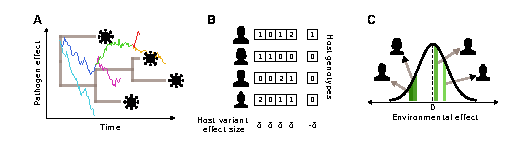
\includegraphics[width = \linewidth]{figures/simulation_setup.pdf}
%DIFDELCMD < 	%%%
\DIFdelendFL \DIFaddbeginFL 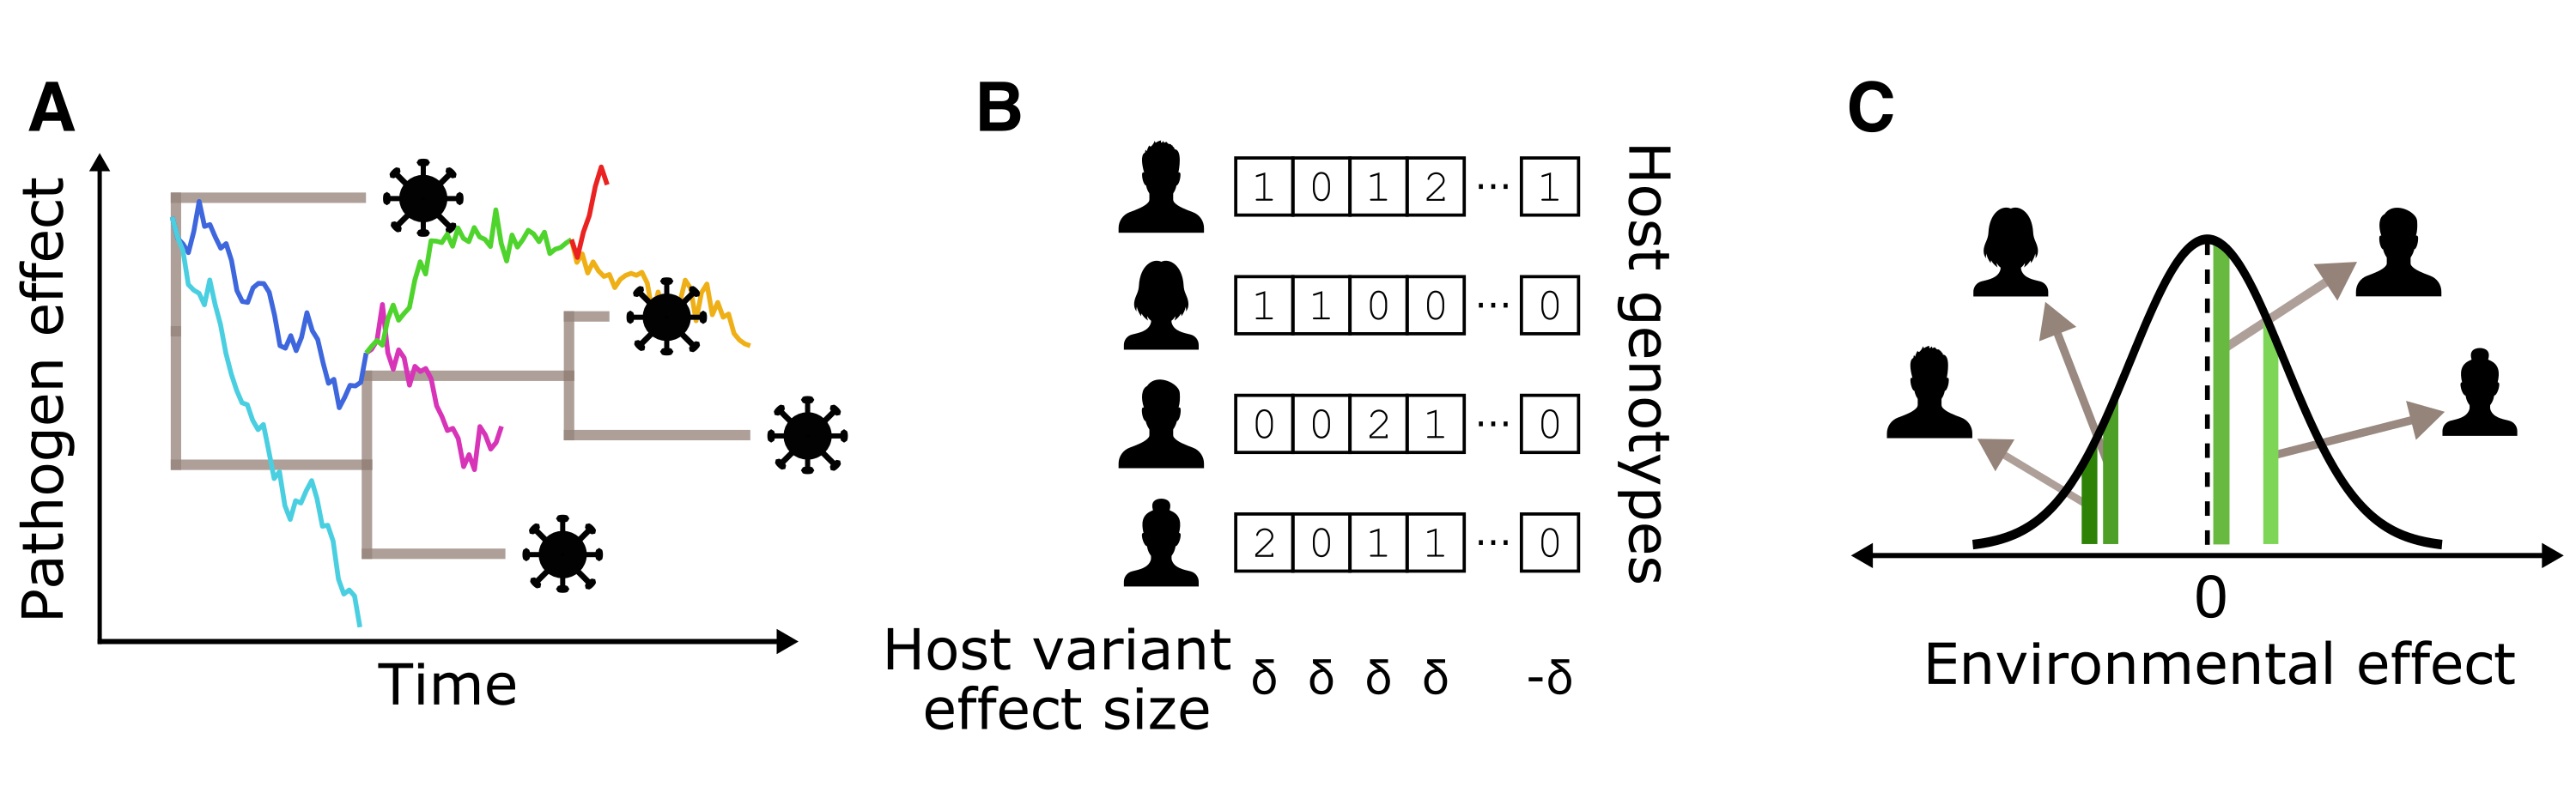
\includegraphics[width = \linewidth]{figures/simulation_setup.png}
	\DIFaddendFL \caption{A high-level schematic of our \DIFdelbeginFL \DIFdelFL{POUMM-based }\DIFdelendFL \DIFaddbeginFL \DIFaddFL{phylogenetic Ornstein-Uhlenbeck mixed model (POUMM)-based }\DIFaddendFL simulation framework \DIFaddbeginFL \DIFaddFL{in the context of HIV-1 set-point viral load (spVL)}\DIFaddendFL . (A) shows how \DIFdelbeginFL \DIFdelFL{pathogen genetic }\DIFdelendFL \DIFaddbeginFL \DIFaddFL{the viral }\DIFaddendFL effects on spVL evolve along the \DIFdelbeginFL \DIFdelFL{pathogen }\DIFdelendFL \DIFaddbeginFL \DIFaddFL{viral }\DIFaddendFL phylogeny according to an \DIFdelbeginFL \DIFdelFL{Ornstein Uhlenbeck }\DIFdelendFL \DIFaddbeginFL \DIFaddFL{Ornstein-Uhlenbeck }\DIFaddendFL process. (B) shows \DIFaddbeginFL \DIFaddFL{how human }\DIFaddendFL host genetic effects \DIFdelbeginFL \DIFdelFL{, which }\DIFdelendFL are the sum of independent effects from several causal variants. Each variant can be present in 0, 1, or 2 copies\DIFdelbeginFL \DIFdelFL{and we assume half }\DIFdelendFL \DIFaddbeginFL \DIFaddFL{. Half the variants }\DIFaddendFL have \DIFaddbeginFL \DIFaddFL{a positive }\DIFaddendFL effect \DIFaddbeginFL \DIFaddFL{of }\DIFaddendFL size $\delta$ \DIFdelbeginFL \DIFdelFL{on the trait value }\DIFdelendFL and half have \DIFaddbeginFL \DIFaddFL{a negative }\DIFaddendFL effect \DIFaddbeginFL \DIFaddFL{of }\DIFaddendFL size \DIFdelbeginFL \DIFdelFL{$-\delta$}\DIFdelendFL \DIFaddbeginFL \DIFaddFL{$\delta$}\DIFaddendFL . (C) shows \DIFdelbeginFL \DIFdelFL{that }\DIFdelendFL \DIFaddbeginFL \DIFaddFL{how other }\DIFaddendFL environmental effects are \DIFdelbeginFL \DIFdelFL{assumed to be independent between sampled individuals and are }\DIFdelendFL \DIFaddbeginFL \DIFaddFL{independently }\DIFaddendFL drawn from a \DIFaddbeginFL \DIFaddFL{Gaussian }\DIFaddendFL distribution centered at \DIFdelbeginFL \DIFdelFL{zero. Measured trait values are the sum of these }\DIFdelendFL \DIFaddbeginFL \DIFaddFL{0. These }\DIFaddendFL three effects \DIFaddbeginFL \DIFaddFL{sum to the trait value }\DIFaddendFL for each simulated individual.}
		\label{fig:spVLModel}
	\end{center}
\end{figure}

\DIFdelbegin \DIFdel{So far, PMMs with two }\DIFdelend \DIFaddbegin \DIFadd{PMMs have previously been applied to the study of infectious disease traits using two different }\DIFaddend types of random processes \DIFdelbegin \DIFdel{have been used to model spVL }\DIFdelend \DIFaddbegin \DIFadd{to model trait }\DIFaddend evolution. The Brownian Motion (BM) process assumes unbounded trait values, i.e. \DIFdelbegin \DIFdel{spVL }\DIFdelend \DIFaddbegin \DIFadd{the trait }\DIFaddend can attain any value. The Ornstein-Uhlenbeck (OU) process assumes trait values fluctuate around an optimal value, i.e. extreme \DIFdelbegin \DIFdel{spVL }\DIFdelend \DIFaddbegin \DIFadd{trait }\DIFaddend values are unlikely. \DIFdelbegin \DIFdel{\mbox{%DIFAUXCMD
\citep{Mitov2018} }\hskip0pt%DIFAUXCMD
and \mbox{%DIFAUXCMD
\citep{Bertels2018} }\hskip0pt%DIFAUXCMD
}\DIFdelend \DIFaddbegin \DIFadd{Here, we assume the more flexible OU process as it encompasses a wider variety of evolutionary scenarios. For example, \mbox{%DIFAUXCMD
\citet{Mitov2018} }\hskip0pt%DIFAUXCMD
and \mbox{%DIFAUXCMD
\citet{Bertels2018} }\hskip0pt%DIFAUXCMD
}\DIFaddend previously showed the OU process has higher statistical support for \DIFaddbegin \DIFadd{HIV-1 }\DIFaddend spVL. This makes sense given that spVL is likely under stabilizing selection to maximize viral transmission potential \citep{Fraser2014}. \DIFdelbegin \DIFdel{Therefore, we assume the OU process. }\DIFdelend The full model is called the phylogenetic Ornstein-Uhlenbeck mixed model (POUMM) and is described in detail by \citet{Mitov2018}. Here, we review the main \DIFdelbegin \DIFdel{relevant points in the spVL context}\DIFdelend \DIFaddbegin \DIFadd{points relevant to our method}\DIFaddend .

Under the POUMM, the \DIFdelbegin \DIFdel{spVL }\DIFdelend trait $z$ is the sum of \DIFdelbegin \DIFdel{viral effects $g_v$, host genetic effects $g_h$, and other environmentalor interaction }\DIFdelend \DIFaddbegin \DIFadd{heritable genetic effects $g$, i.e. due to the pathogen, and non-heritable ``environmental'' }\DIFaddend effects $\epsilon$\DIFdelbegin \DIFdel{. We can group the non-heritable effects $g_h$ and $\epsilon$ into a broader category of ``environmental '' effects$e$: 
}\DIFdelend \DIFaddbegin \DIFadd{, i.e. host genetic effects and other environmental or interaction effects: 
}

\DIFaddend \begin{equation}
    z = g \DIFdelbegin \DIFdel{_{v} }\DIFdelend + \DIFdelbegin \DIFdel{e
}\DIFdelend \DIFaddbegin \DIFadd{\epsilon
}\DIFaddend \end{equation}
\DIFdelbegin \DIFdel{$g_v$ is a viral }\DIFdelend \DIFaddbegin \DIFadd{$g$ is a pathogen }\DIFaddend trait that evolves along the phylogeny according to an OU process. The OU process is defined by a stochastic differential equation with two terms. The first term represents a deterministic pull towards an optimal trait value and the second term represents stochastic fluctuations modelled by Brownian motion \citep{Butler2004}:
\DIFaddbegin 

\DIFaddend \begin{align}
\DIFdelbegin %DIFDELCMD < \begin{split}
%DIFDELCMD < 	&dg_v(t) = \alpha[\theta - g_v(t)]dt + \sigma dW_t \\
%DIFDELCMD < 	&g_v(0) = g_0 
%DIFDELCMD < 	\label{eq:OUprocess}
%DIFDELCMD < \end{split}%%%
\DIFdelend \DIFaddbegin \begin{split}
	&dg(t) = \alpha[\theta - g(t)]dt + \sigma dW_t \\
	&g(0) = g_0 
	\label{eq:OUprocess}
\end{split}\DIFaddend 
\end{align}

Here the parameter $\alpha$ represents selection strength towards an evolutionarily optimal value represented by parameter $\theta$. The parameter $\sigma$ measures the intensity of stochastic fluctuations in the evolutionary process. Finally, $dW_t$ is the Wiener process underlying Brownian motion. The OU process is a Gaussian process, meaning that \DIFdelbegin \DIFdel{$g_v(t)$ }\DIFdelend \DIFaddbegin \DIFadd{$g(t)$ }\DIFaddend is a Gaussian random variable. Assuming \DIFdelbegin \DIFdel{$g_v(t)$ }\DIFdelend \DIFaddbegin \DIFadd{$g(t)$ }\DIFaddend starts at initial value $g_0$ at time $t = 0$ at the root of the phylogeny, we can write the expectation for \DIFdelbegin \DIFdel{$g_v(t)$ }\DIFdelend \DIFaddbegin \DIFadd{$g(t)$ }\DIFaddend at time $t$: 
\DIFaddbegin 

\DIFaddend \begin{equation}
   E[g\DIFdelbegin \DIFdel{_v}\DIFdelend (t)] = g_0e^{-\alpha t} + (1 - e^{-\alpha t})\theta \label{eq:OUmean}
\end{equation}
and the variance in \DIFdelbegin \DIFdel{$g_v(t)$ }\DIFdelend \DIFaddbegin \DIFadd{$g(t)$ }\DIFaddend if we were to repeat the random evolutionary process many times \citep{Butler2004}:
\begin{equation}
    Var[g\DIFdelbegin \DIFdel{_v}\DIFdelend (t)] = \frac{\sigma^2}{2\alpha}(1 - e^{-2\alpha t}) \label{eq:OUVar}
\end{equation}

\DIFdelbegin \DIFdel{$g_v$ }\DIFdelend \DIFaddbegin \DIFadd{$g$ }\DIFaddend evolves independently in descendent lineages after a divergence event in the phylogeny. The covariance between \DIFdelbegin \DIFdel{$g_v(t)$ }\DIFdelend \DIFaddbegin \DIFadd{$g(t)$ }\DIFaddend in a lineage $i$ at time $t_i$ and another lineage $j$ at time $t_j$, \DIFdelbegin \DIFdel{$Cov\big(g_{v_i}(t_i), g_{v_j}(t_j)\big)$}\DIFdelend \DIFaddbegin \DIFadd{$Cov\big(g_{i}(t_i), g_{j}(t_j)\big)$}\DIFaddend , increases with the amount of time between $t_0$ and the divergence of the two lineages, $t_{0(ij)}$, and decreases with the total amount of time the lineages evolve independently, $d_{ij}$ \citep{Butler2004}: 
\DIFaddbegin 

\DIFaddend \begin{equation}
	Cov\big(g\DIFdelbegin \DIFdel{_{v_i}}\DIFdelend \DIFaddbegin \DIFadd{_{i}}\DIFaddend (t_i), g\DIFdelbegin \DIFdel{_{v_j}}\DIFdelend \DIFaddbegin \DIFadd{_{j}}\DIFaddend (t_j)\big) = \frac{\sigma^2}{2\alpha}[e^{-\alpha d_{ij}}(1 - e^{-2\alpha t_{0(ij)}})]
	\label{eq:OUcov}
\end{equation}
Next, we \DIFdelbegin \DIFdel{remember that $e$ }\DIFdelend \DIFaddbegin \DIFadd{recall that $\epsilon$ }\DIFaddend is the non-heritable \DIFdelbegin \DIFdel{, environmental part of spVL. $e$ }\DIFdelend \DIFaddbegin \DIFadd{part of the trait. $\epsilon$ }\DIFaddend is modeled as a Gaussian random variable that is time- and phylogeny-independent. The expectation of \DIFdelbegin \DIFdel{$e$ }\DIFdelend \DIFaddbegin \DIFadd{$\epsilon$ }\DIFaddend is 0, meaning \DIFdelbegin \DIFdel{environmental }\DIFdelend \DIFaddbegin \DIFadd{non-heritable }\DIFaddend effects are equally likely to raise or lower \DIFdelbegin \DIFdel{spVL from the virus-determined }\DIFdelend \DIFaddbegin \DIFadd{the trait from the pathogen-determined }\DIFaddend level. The parameter \DIFdelbegin \DIFdel{$\sigma_e^2$ }\DIFdelend \DIFaddbegin \DIFadd{$\sigma_\epsilon^2$ }\DIFaddend measures the between-host variance of the \DIFdelbegin \DIFdel{environmental effect.
}\DIFdelend \DIFaddbegin \DIFadd{non-heritable effect.
}

\DIFaddend \begin{align}
\DIFdelbegin %DIFDELCMD < \begin{split}
%DIFDELCMD < 	E(e) = 0 \\
%DIFDELCMD < 	Var(e) = \sigma^2_e
%DIFDELCMD < \end{split}%%%
\DIFdelend \DIFaddbegin \begin{split}
	E(\epsilon) = 0 \\
	Var(\epsilon) = \sigma^2_\epsilon
\end{split}\DIFaddend 
\end{align}

Finally, broad-sense trait heritability can be calculated as the fraction of total trait variance that is heritable:
\DIFaddbegin 

\DIFaddend \begin{equation}
	H^2\DIFdelbegin \DIFdel{_{\bar{t}} }\DIFdelend \DIFaddbegin \DIFadd{_{t} }\DIFaddend = \DIFdelbegin \DIFdel{\frac{Var[g_v(t)]}{Var[g_v(t)] + Var(e)} }\DIFdelend \DIFaddbegin \DIFadd{\frac{Var[g(t)]}{Var[g(t)] + Var(\epsilon)} }\DIFaddend = \DIFdelbegin \DIFdel{\frac{\frac{\sigma^2}{2\alpha}(1 - e^{-2\alpha t})}{\frac{\sigma^2}{2\alpha}(1 - e^{-2\alpha t}) + \sigma^2_e}
}\DIFdelend \DIFaddbegin \DIFadd{\frac{\frac{\sigma^2}{2\alpha}(1 - e^{-2\alpha t})}{\frac{\sigma^2}{2\alpha}(1 - e^{-2\alpha t}) + \sigma^2_\epsilon}
	}\label{eq:POUMM-H2}
\DIFaddend \end{equation}

\subsection*{Teasing apart pathogen and non-pathogen effects on \DIFdelbegin \DIFdel{spVL}\DIFdelend \DIFaddbegin \DIFadd{a trait}\DIFaddend }

Given the assumptions of the POUMM, we can estimate a heritable pathogen effect on \DIFdelbegin \DIFdel{spVL and a }\DIFdelend \DIFaddbegin \DIFadd{a trait and a corresponding }\DIFaddend non-heritable, host and environmental effect\DIFdelbegin \DIFdel{on spVL}\DIFdelend . Here, we derive a maximum-likelihood estimate for these values for individuals in a \DIFaddbegin \DIFadd{GWAS }\DIFaddend cohort, given measured \DIFdelbegin \DIFdel{spVL }\DIFdelend \DIFaddbegin \DIFadd{trait }\DIFaddend values and a pathogen phylogeny linking the infecting strains.

Let \DIFdelbegin \DIFdel{$\bm{g}_v(\bm{t})$ }\DIFdelend \DIFaddbegin \DIFadd{$\bm{g}(\bm{t})$ }\DIFaddend be a vector of \DIFdelbegin \DIFdel{$g_v$ }\DIFdelend \DIFaddbegin \DIFadd{$g$ }\DIFaddend values, one for each individual in the cohort. $\bm{t}$ are the sampling times of each individual relative to the root of the phylogeny. To simplify notation, we omit the $\bm{t}$ from here on. \DIFdelbegin \DIFdel{$\bm{g}_v$ }\DIFdelend \DIFaddbegin \DIFadd{$\bm{g}$ }\DIFaddend is a realization of a Gaussian random vector \DIFdelbegin \DIFdel{$\bm{G_v} \sim \mathcal{N}\big(\bm{\mu}_{OU}, \boldsymbol{\Sigma}_{OU}\big)$}\DIFdelend \DIFaddbegin \DIFadd{$\bm{G} \sim \mathcal{N}\big(\bm{\mu}_{OU}, \boldsymbol{\Sigma}_{OU}\big)$}\DIFaddend . The expectation $\bm{\mu}_{OU}$ is defined by equation \ref{eq:OUmean}, the diagonal elements of the covariance matrix $\boldsymbol{\Sigma}_{OU}$ are defined by equation \ref{eq:OUVar}, and the off-diagonal elements of $\boldsymbol{\Sigma}_{OU}$ by equation \ref{eq:OUcov}. \DIFdelbegin %DIFDELCMD < 

%DIFDELCMD < %%%
\DIFdelend Similarly, let \DIFdelbegin \DIFdel{$\bm{e}$ }\DIFdelend \DIFaddbegin \DIFadd{$\bm{\epsilon}$ }\DIFaddend be a vector of the \DIFdelbegin \DIFdel{environmental part of spVL }\DIFdelend \DIFaddbegin \DIFadd{non-heritable part of the trait }\DIFaddend for each individual.  \DIFdelbegin \DIFdel{$\bm{e}$ }\DIFdelend \DIFaddbegin \DIFadd{$\bm{\epsilon}$ }\DIFaddend is a realization of a Gaussian random vector \DIFdelbegin \DIFdel{$\bm{E} \sim \mathcal{N}\big(\bm{0}, \boldsymbol{\Sigma}_E\big)$, where $\boldsymbol{\Sigma}_E$ }\DIFdelend \DIFaddbegin \DIFadd{$\bm{\mathcal{E}} \sim \mathcal{N}\big(\bm{0}, \boldsymbol{\Sigma}_\mathcal{E}\big)$, where $\boldsymbol{\Sigma}_\mathcal{E}$ }\DIFaddend is a diagonal matrix with diagonal elements equal to \DIFdelbegin \DIFdel{$\sigma^2_e$}\DIFdelend \DIFaddbegin \DIFadd{$\sigma^2_\epsilon$}\DIFaddend .

Considering that \DIFdelbegin \DIFdel{$\bm{G_v}$ and $\bm{E}$ }\DIFdelend \DIFaddbegin \DIFadd{$\bm{G}$ and $\bm{\mathcal{E}}$ }\DIFaddend are independent random vectors and that their realizations \DIFdelbegin \DIFdel{$\bm{g}_v$ and $\bm{e}$ }\DIFdelend \DIFaddbegin \DIFadd{$\bm{g}$ and $\bm{\epsilon}$ }\DIFaddend must sum together to equal the observed \DIFdelbegin \DIFdel{spVL }\DIFdelend \DIFaddbegin \DIFadd{trait }\DIFaddend values $\bm{z}$, we can write the following proportionality for the joint probability density of \DIFdelbegin \DIFdel{$\bm{g}_v$ and $\bm{e}$:
}\DIFdelend \DIFaddbegin \DIFadd{$\bm{g}$ and $\bm{\epsilon}$:
}

\DIFaddend \begin{equation}
	f\big(\bm{g}\DIFdelbegin \DIFdel{_v}\DIFdelend , \DIFdelbegin %DIFDELCMD < \bm{e}%%%
\DIFdelend \DIFaddbegin \bm{\epsilon}\DIFaddend \big) \propto \mathcal{N}\big(\bm{g}\DIFdelbegin \DIFdel{_v}\DIFdelend ; \bm{\mu}_{G}, \boldsymbol{\Sigma}_G\big)
	\label{eq:pdfGprop}
\end{equation} 

where the expected value of \DIFdelbegin \DIFdel{$\bm{g}_v$ }\DIFdelend \DIFaddbegin \DIFadd{$\bm{g}$ }\DIFaddend and the covariance matrix $\boldsymbol{\Sigma}_G$ are defined as:
\DIFaddbegin 

\DIFaddend \begin{align}
	Exp(\bm{g}\DIFdelbegin \DIFdel{_v}\DIFdelend ) = \bm{\mu}_{G} &=  \boldsymbol{\Sigma}_G\big(\boldsymbol{\Sigma}_{OU}^{-1}\bm{\mu}_{OU} + \boldsymbol{\Sigma}\DIFdelbegin \DIFdel{_E}\DIFdelend \DIFaddbegin \DIFadd{_\mathcal{E}}\DIFaddend ^{-1} \bm{z}\big) \label{eq:MuG}\\
	\boldsymbol{\Sigma}_G &= \big(\boldsymbol{\Sigma}_{OU}^{-1} + \boldsymbol{\Sigma}\DIFdelbegin \DIFdel{_E}\DIFdelend \DIFaddbegin \DIFadd{_\mathcal{E}}\DIFaddend ^{-1}\big)^{-1} \label{eq:SigmaG}
\end{align}

\begin{proof}
	\begin{align}\label{eq:pdfG}
	\DIFdelbegin %DIFDELCMD < \begin{split}
%DIFDELCMD < 		f\big(\bm{g}_v,\ \bm{e}\big) &= f\big(\bm{g}_v|\ \bm{e}\big) \times f\big(\bm{e}\big) \\
%DIFDELCMD < 	&= f\big(\bm{g}_v\big) \times f\big(\bm{e}\big) \\
%DIFDELCMD < 	&= \mathcal{N}\big(\bm{g}_v;\ \bm{\mu}_{OU}, \mathbf{\Sigma}_{OU}\big) \times \mathcal{N}\big(\bm{e};\ \bm{0}, \mathbf{\Sigma}_E\big) \\
%DIFDELCMD < 	&= \mathcal{N}\big(\bm{g}_v;\ \bm{\mu}_{OU}, \mathbf{\Sigma}_{OU}\big) \times \mathcal{N}\big(\bm{z} - \bm{g}_v;\ \bm{0}, \mathbf{\Sigma}_E\big) \\
%DIFDELCMD < 	&= \mathcal{N}\big(\bm{g}_v;\ \bm{\mu}_{OU}, \mathbf{\Sigma}_{OU}\big) \times \mathcal{N}\big(\bm{g}_v;\ \bm{z}, \mathbf{\Sigma}_E\big)
%DIFDELCMD < 	\end{split}%%%
\DIFdelend \DIFaddbegin \begin{split}
		f\big(\bm{g},\ \bm{\epsilon}\big) &= f\big(\bm{g}|\ \bm{\epsilon}\big) \times f\big(\bm{\epsilon}\big) \\
	&= f\big(\bm{g}\big) \times f\big(\bm{\epsilon}\big) \\
	&= \mathcal{N}\big(\bm{g};\ \bm{\mu}_{OU}, \mathbf{\Sigma}_{OU}\big) \times \mathcal{N}\big(\bm{\epsilon};\ \bm{0}, \mathbf{\Sigma}_\mathcal{E}\big) \\
	&= \mathcal{N}\big(\bm{g};\ \bm{\mu}_{OU}, \mathbf{\Sigma}_{OU}\big) \times \mathcal{N}\big(\bm{z} - \bm{g};\ \bm{0}, \mathbf{\Sigma}_\mathcal{E}\big) \\
	&= \mathcal{N}\big(\bm{g};\ \bm{\mu}_{OU}, \mathbf{\Sigma}_{OU}\big) \times \mathcal{N}\big(\bm{g};\ \bm{z}, \mathbf{\Sigma}_\mathcal{E}\big)
	\end{split}\DIFaddend 
\end{align}

	Equations \ref{eq:MuG} and \ref{eq:SigmaG} follow from eq. \ref{eq:pdfG} and eq. 371, p. 42, section 8.1.8 ``Product of Gaussian densities'' in \DIFdelbegin \DIFdel{\mbox{%DIFAUXCMD
\citep{Petersen2012}}\hskip0pt%DIFAUXCMD
}\DIFdelend \DIFaddbegin \DIFadd{\mbox{%DIFAUXCMD
\citet{Petersen2012}}\hskip0pt%DIFAUXCMD
}\DIFaddend .
\end{proof}

Importantly, equation \ref{eq:MuG} is the maximum likelihood estimate for \DIFdelbegin \DIFdel{$\bm{g}_v$, the viral effect on spVL}\DIFdelend \DIFaddbegin \DIFadd{$\bm{g}$, the pathogen effect on the trait}\DIFaddend , taking into account all available information - measured \DIFdelbegin \DIFdel{spVL}\DIFdelend \DIFaddbegin \DIFadd{trait values}\DIFaddend , the pathogen phylogeny, and inferred POUMM parameters. This estimator is an inverse-variance weighted average of measured \DIFdelbegin \DIFdel{spVL }\DIFdelend \DIFaddbegin \DIFadd{trait }\DIFaddend ($\bm{z}$) and information from the POUMM evolutionary model ($\bm{\mu}_{OU}$). In other words, \DIFdelbegin \DIFdel{$g_v$ }\DIFdelend \DIFaddbegin \DIFadd{$\bm{g}$ }\DIFaddend will be closer to \DIFdelbegin \DIFdel{measured spVL if spVL }\DIFdelend \DIFaddbegin \DIFadd{the measured trait value if the trait }\DIFaddend is not very heritable. If \DIFdelbegin \DIFdel{spVL }\DIFdelend \DIFaddbegin \DIFadd{the trait }\DIFaddend is highly heritable, \DIFdelbegin \DIFdel{$g_v$ }\DIFdelend \DIFaddbegin \DIFadd{$\bm{g}$ }\DIFaddend will be closer to the expected value under the POUMM, i.e. take more information from the phylogenetic relationships between infecting strains. 

Given the estimator we just derived for \DIFdelbegin \DIFdel{$\bm{g}_v$}\DIFdelend \DIFaddbegin \DIFadd{$\bm{g}$}\DIFaddend , we can now estimate \DIFdelbegin \DIFdel{$\bm{e}$, the spVL }\DIFdelend \DIFaddbegin \DIFadd{$\bm{\epsilon}$, the trait }\DIFaddend value $without$ pathogen effects: 
\DIFaddbegin 

\DIFaddend \begin{equation}
	\DIFdelbegin %DIFDELCMD < \hat{\bm{e}} %%%
\DIFdelend \DIFaddbegin \hat{\bm{\epsilon}} \DIFaddend = \bm{z} - Exp(\bm{g}\DIFdelbegin \DIFdel{_v}\DIFdelend )
	\label{eq:EHat}
\end{equation}

We will use this value to try to improve upon standard GWAS methods in infectious disease.

\subsection*{A POUMM-based GWAS framework for infectious disease}

We propose to improve standard GWAS for infectious diseases by estimating and removing trait variability due to pathogen effects. Our new framework is as follows:

\begin{enumerate}
	\item Sample \DIFaddbegin \DIFadd{paired }\DIFaddend host genotypes, \DIFdelbegin \DIFdel{trait values, and pathogen genome sequence data }\DIFdelend \DIFaddbegin \DIFadd{pathogen genome sequences, and trait values }\DIFaddend from a cohort.
	\item Construct a pathogen phylogeny using the pathogen genome sequences.
	\item Estimate the parameters of the POUMM based on the trait values and the pathogen phylogeny. This can be done with \DIFdelbegin \DIFdel{e.g. }\DIFdelend the R package POUMM \citep{Mitov2017a-POUMM}.
	\item Generate maximum-likelihood estimates for the pathogen and corresponding non-pathogen effects on the trait using equations \ref{eq:MuG} and \ref{eq:EHat}.
	\item Perform GWAS with only the non-pathogen effects on the trait as the response variable.
\end{enumerate}

\section*{Results}

\subsection*{Simulation study}

To test the theoretical best-case performance of our method, we simulated data under the POUMM and applied our framework to the simulated data. \DIFdelbegin \DIFdel{Figure \ref{fig:spVLModel} shows a high-level schematic of our simulation framework and Table \ref{tab:sim-params} gives the value or expression for each parameter. 
In a nutshell}\DIFdelend \DIFaddbegin \DIFadd{We parameterized our simulation scheme with the time-scale and other parameters of an HIV-1 outbreak in mind, with spVL as the trait of interest. 
}

\DIFadd{We first simulated a phylogeny of 500 tips with exponentially distributed branch lengths and mean root-to-tip time of 0.14 substitutions per site per year as in \mbox{%DIFAUXCMD
\cite{Hodcroft2014}}\hskip0pt%DIFAUXCMD
. Then}\DIFaddend , we simulated \DIFdelbegin \DIFdel{independent, additive host genetic effects, independent environmental effects, and heritable pathogen genetic effects under different scenarios of trait heritability and selection strength }\DIFdelend \DIFaddbegin \DIFadd{pathogen trait values $\bm{g}$ along this phylogeny using the POUMM package in R \mbox{%DIFAUXCMD
\citep{Mitov2017a-POUMM}}\hskip0pt%DIFAUXCMD
. This part of the simulation is illustrated in Figure \ref{fig:spVLModel}A. For the simulation, we considered a range of pathogen heritability parameter values $H^2$, from 15 to 75\%, and a range of selection strength parameters values $\alpha$, from 0.1 to 60 time$^{-1}$. The intensity of stochastic fluctuations parameter $\sigma$ was determined based on $H^2$ and $\alpha$ (a re-arrangement of equation \ref{eq:OUVar}, equation given in Table \ref{tab:sim-params}). As shown in Figure \ref{fig:sigma-vs-alpha}, higher $\alpha$ values correspond to higher $\sigma$ values to maintain constant $H^2$ under this parameterization. For each $H^2$ and $\alpha$ value considered in the simulation, we recorded the simulated pathogen part of the trait value for each tip in the phylogeny.
}

\DIFadd{We paired each tip's simulated pathogen trait value with a simulated host trait value. Simulated hosts had 20 genome positions. We sampled alleles (0, 1, or 2) for each position from a binomial distribution with probability 0.13}\DIFaddend . \DIFdelbegin \DIFdel{To maintain the same heritability while varying selection strength, we counter-balanced by varying the intensity of stochastic evolutionary fluctuations accordingly.
We fixed other variables to plausible values }\DIFdelend \DIFaddbegin \DIFadd{10 random positions had an effect size of 0.2 on the trait and 10 had an effect size of -0.2. This part of the simulation is illustrated in Figure \ref{fig:spVLModel}B. Our parameterization produced roughly normally distributed host trait values centered at 0 with variance equal to 25\% of the total trait variance, which we constrained to 0.73 }\DIFaddend based on the \DIFdelbegin \DIFdel{spVL literature. }\DIFdelend \DIFaddbegin \DIFadd{variance in log spVL values measured by \mbox{%DIFAUXCMD
\cite{Mitov2018}}\hskip0pt%DIFAUXCMD
. We used 25\% host heritability for spVL based on \mbox{%DIFAUXCMD
\cite{McLaren2015}}\hskip0pt%DIFAUXCMD
.
}\DIFaddend 

\DIFaddbegin \DIFadd{Finally, we sampled an additional random environmental effect for each tip from a normal distribution centered at 0, as illustrated in Figure \ref{fig:spVLModel}C. The variance of this distribution was scaled based on the pathogen heritability of the trait, from 0 (no affect) in the scenario with 75\% pathogen heritability and 25\% host heritability to 0.44 in the scenario with 15\% pathogen heritability and 25\% host heritability. Figure \ref{fig:sim-design} provides a more detailed schematic of this simulation framework and Table \ref{tab:sim-params} gives the value or expression for each parameter.
}

\DIFaddend \subsubsection*{Estimator accuracy}

First, we evaluated how well our method estimated the additive host genetic effects from the simulated data. Additive host genetic effects represent an ideal (albeit unattainable) baseline for infectious disease GWAS. Figure \ref{fig:simulationResults}A shows that our method incorporating phylogenetic information can more accurately estimate \DIFdelbegin \DIFdel{this }\DIFdelend \DIFaddbegin \DIFadd{these }\DIFaddend value compared to the trait value. To ensure a fair comparison, we scaled trait values to have the same mean, zero, as host genetic effects so as not to bias the root mean squared error (RMSE) by a constant factor. \DIFdelbegin \DIFdel{In }\DIFdelend \DIFaddbegin \DIFadd{As shown in }\DIFaddend the supplemental material, we \DIFdelbegin \DIFdel{show why the }\DIFdelend \DIFaddbegin \DIFadd{can calculate the expected RMSE using the }\DIFaddend scaled trait value \DIFdelbegin \DIFdel{is expected to have an RMSE of approximately }\DIFdelend \DIFaddbegin \DIFadd{across scenarios in our simulation scheme because the variance in the trait due to pathogen genetic effects and environmental effects is fixed. Thus, we expect the RMSE using the scaled trait value to be }\DIFaddend 0.74 \DIFdelbegin \DIFdel{under our simulation scheme}\DIFdelend \DIFaddbegin \DIFadd{across all simulation scenarios}\DIFaddend . By incorporating phylogenetic information, we can improve upon this error in scenarios where the trait is highly heritable\DIFdelbegin \DIFdel{and }\DIFdelend \DIFaddbegin \DIFadd{, }\DIFaddend under low selection pressure\DIFdelbegin \DIFdel{. This is because high heritability means the pathogen greatly effects the trait value. Then, when the trait is under weak selection, pathogen effects can drift far from the long-term optimum and stochastic fluctuations are low to maintain the same heritability }\DIFdelend \DIFaddbegin \DIFadd{, and with relatively moderate stochastic fluctuations compared to outbreak duration. Figure \ref{fig:simulationTraitExample} gives some intuition for how this correction works by contrasting simulated scenarios with high and low heritability and low selection strength/ low stochastic fluctuations. Depending on these parameters, trait values are more or less phylogenetically correlated (see also Figure \ref{fig:tip-trait-correlation}) and the phylogeny is more or less useful for accurately estimating the heritable pathogen and corresponding non-heritable, non-pathogen part of the trait values}\DIFaddend . 
\DIFdelbegin \DIFdel{Thus, our method performs well when an infectious disease trait is highly heritable and trait values are highly correlated amongst closely related members of a transmission chain, but vary widely within the entire cohort.
}\DIFdelend 

\subsubsection*{Theoretical GWAS improvement}

Next, we characterized the evolutionary scenarios under which our framework can actually improve GWAS power. We used the true positive rate (TPR) to evaluate the fraction of simulated \DIFaddbegin \DIFadd{causal }\DIFaddend host genetic variants \DIFdelbegin \DIFdel{with direct effects }\DIFdelend we could recover as being significantly associated with the trait. We performed three different GWAS for each simulated dataset: the first represents an ideal in which we can exactly know and remove pathogen effects from trait values, the second is using our method to estimate this value and remove it, and the third represents a standard GWAS using the scaled trait value. Figure \ref{fig:simulationResults}B shows that our framework can improve the TPR in simulated scenarios where selection strength $<$ 10 time$^{-1}$ and heritability $>$ 45\%. If we were able to perfectly estimate and remove pathogen effects \DIFdelbegin \DIFdel{on }\DIFdelend \DIFaddbegin \DIFadd{from }\DIFaddend a trait, the TPR would increase across all values of selection strength so long as the trait is more than marginally heritable. We estimate approximately 25\% to be the heritability threshold above which GWAS power is negatively impacted by pathogen effects. In summary, we show \DIFaddbegin \DIFadd{that }\DIFaddend it is theoretically possible to improve GWAS power for heritable infectious disease traits by estimating and removing pathogen effects using information from the pathogen phylogeny.

% More accurate estimation of the non-viral part of spVL does not guarantee improved GWAS power. For example, if the viral part of spVL were constant across all viruses, association results (significance and effect size) would not be effected by a viral contribution to the trait. 
% Under our simulation set-up a standard GWAS would have $\approx$ 30\% power to detect a host variant explaining 1.25\% of the variability in spVL. This matches simulation results (figure \ref{fig:simulationResults}B, scaled spVL). 

\begin{figure}[H]
	\begin{center}
		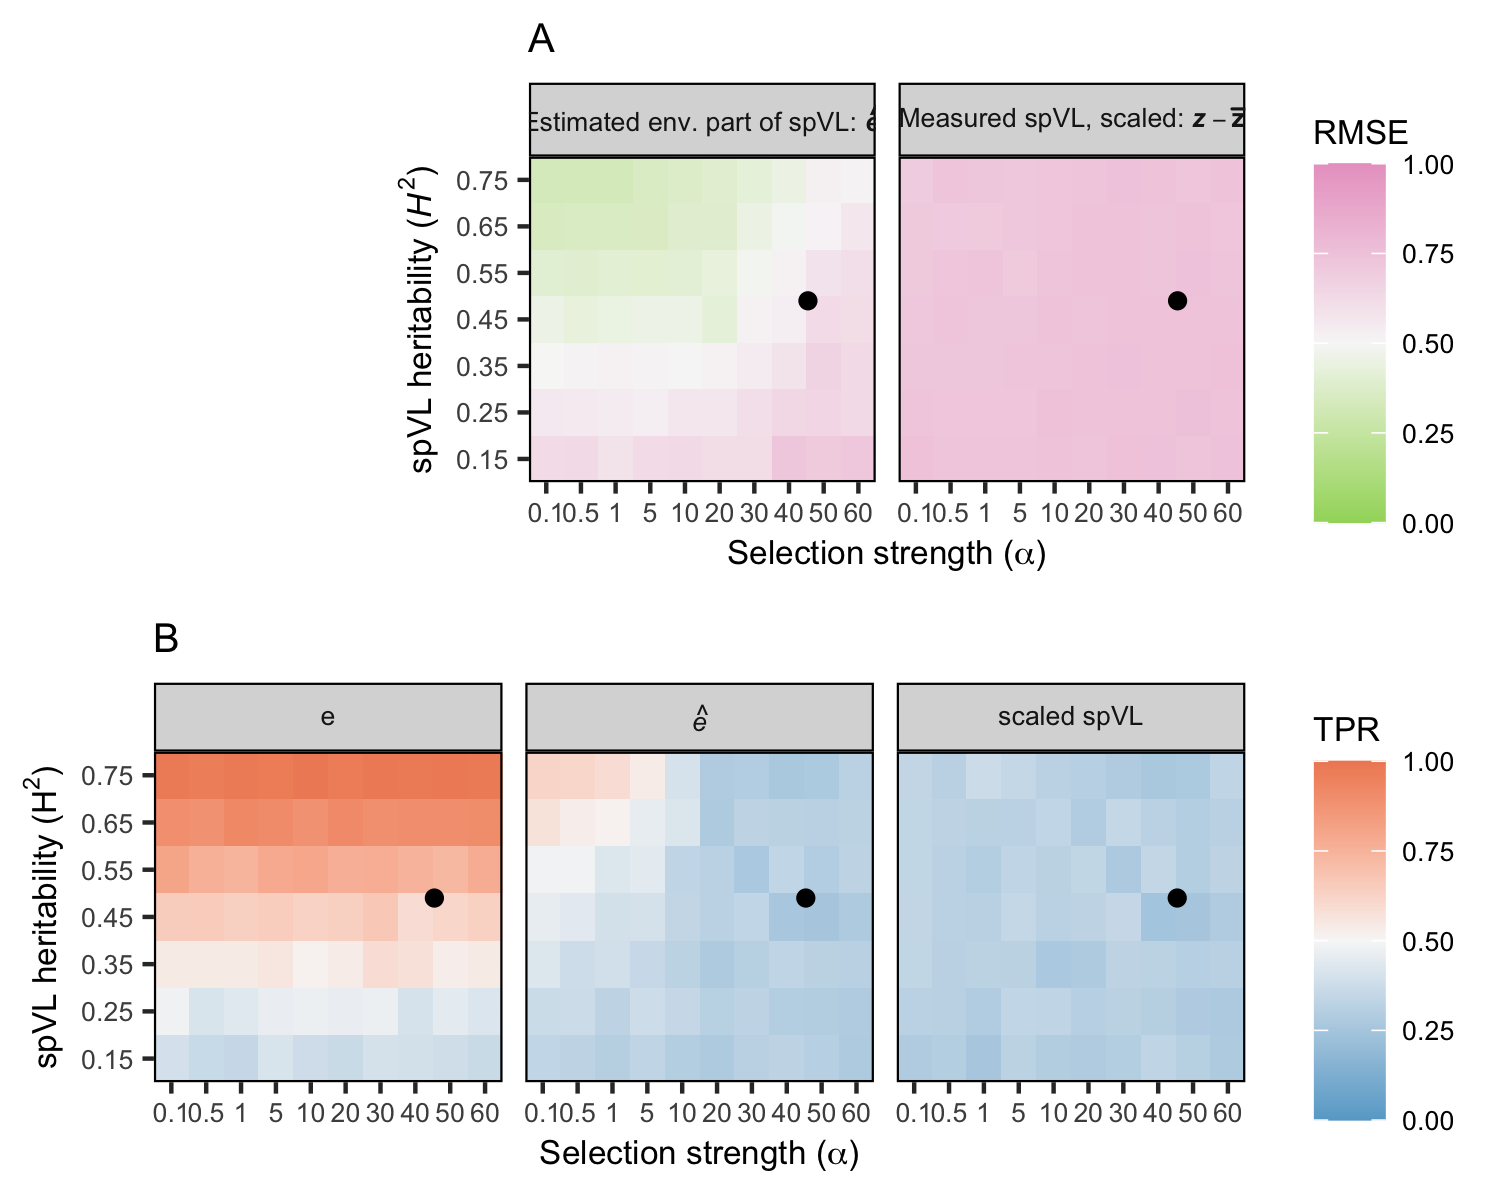
\includegraphics[width=\linewidth]{figures/simulation_results}
		\caption{Results from the simulation study. We simulated host, pathogen, and environmental effects on a trait under the \DIFaddbeginFL \DIFaddFL{phylogenetic Ornstein-Uhlenbeck mixed model (}\DIFaddendFL POUMM\DIFaddbeginFL \DIFaddFL{) }\DIFaddendFL with different heritability (\DIFaddbeginFL \DIFaddFL{$H^2$; }\DIFaddendFL y-axis) and selection strength (\DIFaddbeginFL \DIFaddFL{$\alpha$; }\DIFaddendFL x-axis) parameters. For each simulated dataset, we applied our method to estimate the non-pathogen effects and performed GWAS with these values. (A) shows \DIFdelbeginFL \DIFdelFL{that }\DIFdelendFL \DIFaddbeginFL \DIFaddFL{the root mean squared error (RMSE) of }\DIFaddendFL our \DIFdelbeginFL \DIFdelFL{method }\DIFdelendFL \DIFaddbeginFL \DIFaddFL{estimator }\DIFaddendFL (left) \DIFdelbeginFL \DIFdelFL{can generate more accurate estimates of host genetic effects than the }\DIFdelendFL \DIFaddbeginFL \DIFaddFL{compared to un-corrected }\DIFaddendFL trait \DIFdelbeginFL \DIFdelFL{value}\DIFdelendFL \DIFaddbeginFL \DIFaddFL{values}\DIFaddendFL , scaled by \DIFdelbeginFL \DIFdelFL{its }\DIFdelendFL \DIFaddbeginFL \DIFaddFL{their }\DIFaddendFL mean (right) \DIFaddbeginFL \DIFaddFL{under each simulated evolutionary scenario}\DIFaddendFL . \DIFaddbeginFL \DIFaddFL{The RMSE is with reference to the true }\DIFaddendFL (\DIFaddbeginFL \DIFaddFL{simulated) host part of the trait values. Thus, more accurate estimates (lower RMSE) mean the trait value used for GWAS will be closer to the true host part of the trait value. (}\DIFaddendFL B) shows how \DIFaddbeginFL \DIFaddFL{genome-wide association study (}\DIFaddendFL GWAS\DIFaddbeginFL \DIFaddFL{) }\DIFaddendFL power can improve given the true, simulated non-pathogen effect on spVL (left) and using our estimate for this value (middle) compared to using the scaled trait value (right). Each tile's color corresponds to the average value across 20 simulated datasets of 500 samples. The \DIFdelbeginFL \DIFdelFL{black point represents our estimates for the }\DIFdelendFL \DIFaddbeginFL \DIFaddFL{points highlight specific }\DIFaddendFL heritability and selection strength \DIFdelbeginFL \DIFdelFL{of }\DIFdelendFL \DIFaddbeginFL \DIFaddFL{values from the }\emph{\DIFaddFL{A. thaliana}}\DIFaddFL{-}\emph{\DIFaddFL{X. arboricola}} \DIFaddFL{quantitative disease resistance (QDR) analysis, HIV-1 }\DIFaddendFL spVL \DIFdelbeginFL \DIFdelFL{based on Swiss HIV Cohort Study data. RMSE = Root mean square error}\DIFdelendFL \DIFaddbeginFL \DIFaddFL{analysis}\DIFaddendFL , \DIFdelbeginFL \DIFdelFL{TPR = True positive rate}\DIFdelendFL \DIFaddbeginFL \DIFaddFL{and four simulated scenarios that are presented in more detail in Figure \ref{fig:tip-trait-correlation}}\DIFaddendFL .}
		\label{fig:simulationResults}
	\end{center}
\end{figure}

\DIFdelbegin \subsection*{\DIFdel{GWAS on the Swiss HIV Cohort}}
%DIFAUXCMD
\DIFdelend \DIFaddbegin \begin{figure}[H]
	\begin{center}
		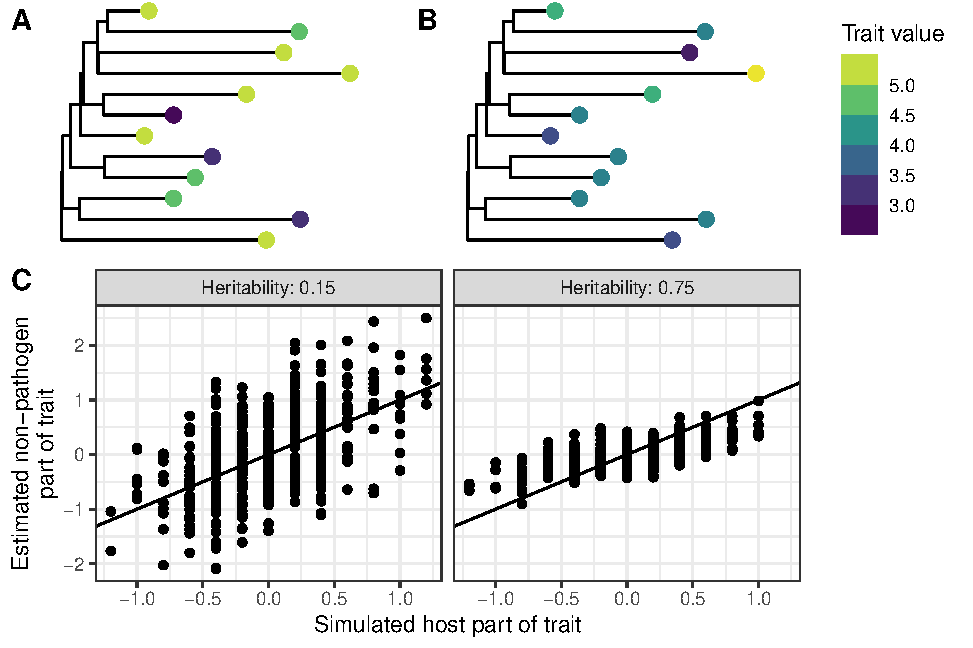
\includegraphics[width=\linewidth]{figures/example_simulation_trait_values.pdf}
		\caption{\DIFaddFL{Simulated data from two evolutionary scenarios where a phylogenetic correction to trait values improves genome-wide association study (GWAS) power (right side) and where it does not (left side). These examples correspond to two of the unfilled points in Figure \ref{fig:simulationResults}. (A) and (B) show total trait values for 12 randomly selected tips from the simulated phylogeny with pathogen heritability $H^2$ of 15 and 75\%, respectively. Depending on the pathogen heritability, trait values are more or less correlated at clustered tips. (C) compares our method's estimate for the non-pathogen part of trait values (y-axis) with true simulated host trait values (x-axis) with pathogen heritability of 15 and 75\%. The solid line is the y=x line. Selection strength $\alpha$ was fixed to 0.1 time $^{-1}$ for both scenarios and all other parameters were fixed as in the full simulation study.}}
		\label{fig:simulationTraitExample}
	\end{center}
\end{figure}
\DIFaddend 

\DIFdelbegin \DIFdel{Finally, we }\DIFdelend \DIFaddbegin \begin{figure}[H]
\begin{center}
    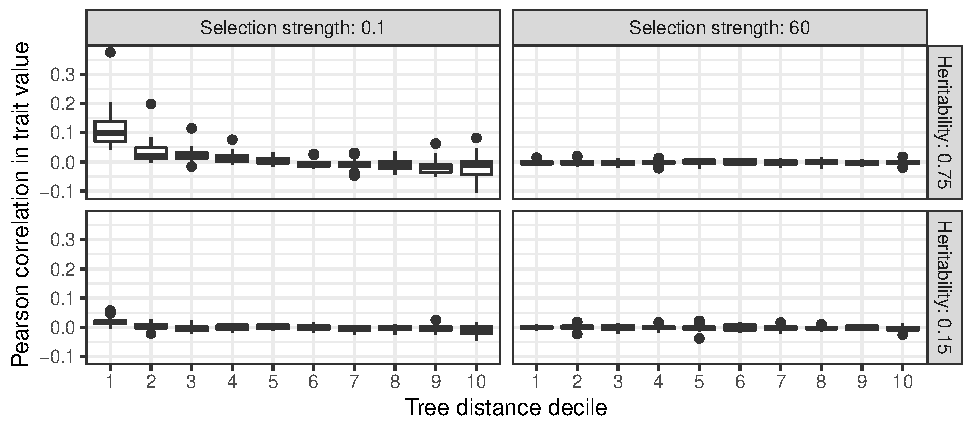
\includegraphics[width = \linewidth]{figures/tip_trait_correlation.pdf}
	\caption{\DIFaddFL{Correlations between trait values in pairs of tips in four simulated scenarios. These examples correspond to the four unfilled points in Figure \ref{fig:simulationResults}. Correlations are calculated for pairs of tips binned by phylogenetic distance (into deciles) across the 20 replicate simulations for each of the four evolutionary scenarios. Trait values are only noticeably correlated for closely clustered tips under the scenario with high pathogen heritability $H^2$ and low selection strength $\alpha$/ low stochastic fluctuations $\sigma$ (upper left facet).}}
	\label{fig:tip-trait-correlation}
	\end{center}
\end{figure}

\subsection*{\DIFadd{Application to HIV-1 set-point viral load}}

\DIFadd{We }\DIFaddend applied our framework to empirical data from \DIFaddbegin \DIFadd{two different host-pathogen systems with different experimental setups (Figure \ref{fig:application-exp-setup}). First, we used data collected by }\DIFaddend the Swiss HIV Cohort Study (SHCS) \DIFdelbegin \DIFdel{. We used data collected }\DIFdelend from 1,\DIFdelbegin \DIFdel{392 }\DIFdelend \DIFaddbegin \DIFadd{493 }\DIFaddend individuals in Switzerland infected with \DIFdelbegin \DIFdel{subtype B HIV-1 }\DIFdelend \DIFaddbegin \DIFadd{HIV-1 subtype B }\DIFaddend between 1994 and 2018. The SHCS provided viral load measurements, $pol$ gene sequences, and human genotype data for these individuals. We followed the \DIFdelbegin \DIFdel{framework }\DIFdelend \DIFaddbegin \DIFadd{method }\DIFaddend outlined above to estimate the pathogen and non-pathogen effects on spVL for the cohort from these data. Figure \ref{fig:spvl-calc-comparison} shows the calculated \DIFaddbegin \DIFadd{(total) }\DIFaddend spVL values, \DIFdelbegin \DIFdel{Figure \ref{fig:spvl-on-tree} shows the inferred pathogen phylogeny, and figures \ref{fig:spvl-on-tree}, \ref{fig:trait-comparison} show the estimated non-pathogen effects on spVL calculated for these individuals}\DIFdelend \DIFaddbegin \DIFadd{which vary between approximately 1 and 6 log copies/mL in the cohort}\DIFaddend .  We estimated spVL heritability in this cohort to be 45\% (95\% highest posterior density, HPD, 24 - 67\%) \DIFdelbegin \DIFdel{\ref{tab:POUMM-parameters-our-estimates}}\DIFdelend \DIFaddbegin \DIFadd{and selection strength to be 58 time$^{-1}$ (95\% HPD 19 - 95) (Figure \ref{fig:poumm-parameters}, Table \ref{tab:POUMM-parameters-our-estimates})}\DIFaddend . To put these values into the context of our simulation study, they are shown as \DIFdelbegin \DIFdel{black }\DIFdelend points on Figure \ref{fig:simulationResults}. \DIFaddbegin \DIFadd{The highest expected correlation in trait values between any two tips in the HIV-1 phylogeny under the POUMM was 0.45. However, Figure \ref{fig:spvl-on-tree} shows that this trait is not obviously phylogenetically structured in the cohort in general, despite high heritability. Finally, figure \ref{fig:trait-comparison} shows that the estimated non-pathogen effects on spVL correlate quite strongly with total spVL. 
}\DIFaddend 

\DIFaddbegin \begin{figure}[H]
\begin{center}
    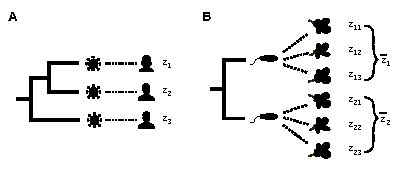
\includegraphics[width = \linewidth]{figures/application_experimental_setups.pdf}
	\caption{\DIFaddFL{A high-level schematic of the experimental setup for the two application datasets. For (A) HIV-1 set-point viral load (spVL) in the Swiss HIV Cohort Study, data are paired viral and human genotypes and associated spVL measurements. We fit the phylogenetic Ornstein-Uhlenbeck mixed model (POUMM) to the viral phylogeny and spVL values associated with each infected individual ($z_1$, $z_2$, ..., $z_{1493}$). For (B) }\emph{\DIFaddFL{A. thaliana}}\DIFaddFL{-}\emph{\DIFaddFL{X. arboricola}} \DIFaddFL{quantitative disease resistance (QDR) from \mbox{%DIFAUXCMD
\cite{Wang2018Two-wayGenomes}}\hskip0pt%DIFAUXCMD
, data are bacterial and plant genotypes with QDR measurements for all possible combinations of pathogen and host plant strains. We fit the POUMM to the bacterial phylogeny and mean QDR calculated for each pathogen strain across all the hosts plant types ($\bar{z}_1$, $\bar{z}_2$, ..., $\bar{z}_{22}$).}}
	\label{fig:application-exp-setup}
	\end{center}
\end{figure}

\DIFaddend We compared our proposed GWAS framework with a more standard approach by performing two different GWAS on the same SHCS human genotypes. \DIFdelbegin \DIFdel{In the }\DIFdelend \DIFaddbegin \DIFadd{We retained 1,392 individuals of European ancestry for the GWAS. In the (i) }\DIFaddend ``GWAS with standard trait value'' we used the \DIFdelbegin \DIFdel{unmodified }\DIFdelend \DIFaddbegin \DIFadd{total }\DIFaddend trait value, \DIFdelbegin \DIFdel{our }\DIFdelend calculated spVL values, as the GWAS response variable. In the \DIFaddbegin \DIFadd{(ii) }\DIFaddend ``GWAS with estimated non-pathogen part of trait'' we used our estimates for the non-pathogen effects on spVL. Figure \ref{fig:gwas-results}A shows that results are qualitatively similar between the two GWAS. Q-Q plots show the distribution of p-values are very similar as well (Figure \ref{fig:qq-plots}). Figure \ref{fig:gwas-results}B shows how the strength of association changed for some variants in the MHC and \emph{CCR5} regions. Taking into account phylogenetic information slightly decreased association strength for most variants in the \emph{CCR5} region. Association strength increased for some variants in the MHC, for example, SNP rs9265880 had the greatest increase in significance in the MHC region, from a p-value of $3.5 \times 10^{-07}$ to $7.7 \times 10^{-09}$. However, the top-associated variants in the MHC and \emph{CCR5} regions were consistent regardless of the GWAS response variable used (\DIFdelbegin \DIFdel{Figure }\DIFdelend \DIFaddbegin \DIFadd{Table }\DIFaddend \ref{tab:gwas-top-associations}). Finally\DIFaddbegin \DIFadd{, }\DIFaddend Table \ref{tab:comp-gwas-mclaren-snps} shows how our GWAS results compare for the two top-associated SNPs identified by \citet{McLaren2015}\DIFdelbegin \DIFdel{. }\DIFdelend \DIFaddbegin \DIFadd{, who performed the largest standard GWAS for HIV spVL to date. Effect sizes are smaller with a phylogenetic correction and p-values are slightly increased. We repeated the analysis using three different approximate maximum-likelihood phylogenies and these results were consistent (see Materials and Methods; Table \ref{tab:comp-gwas-mclaren-snps-alt-trees}). }\DIFaddend In summary, there are no clear patterns that point to new regions of association in the human genome with spVL when we take into account the pathogen phylogeny.

\begin{figure}[H]
	\begin{center}
		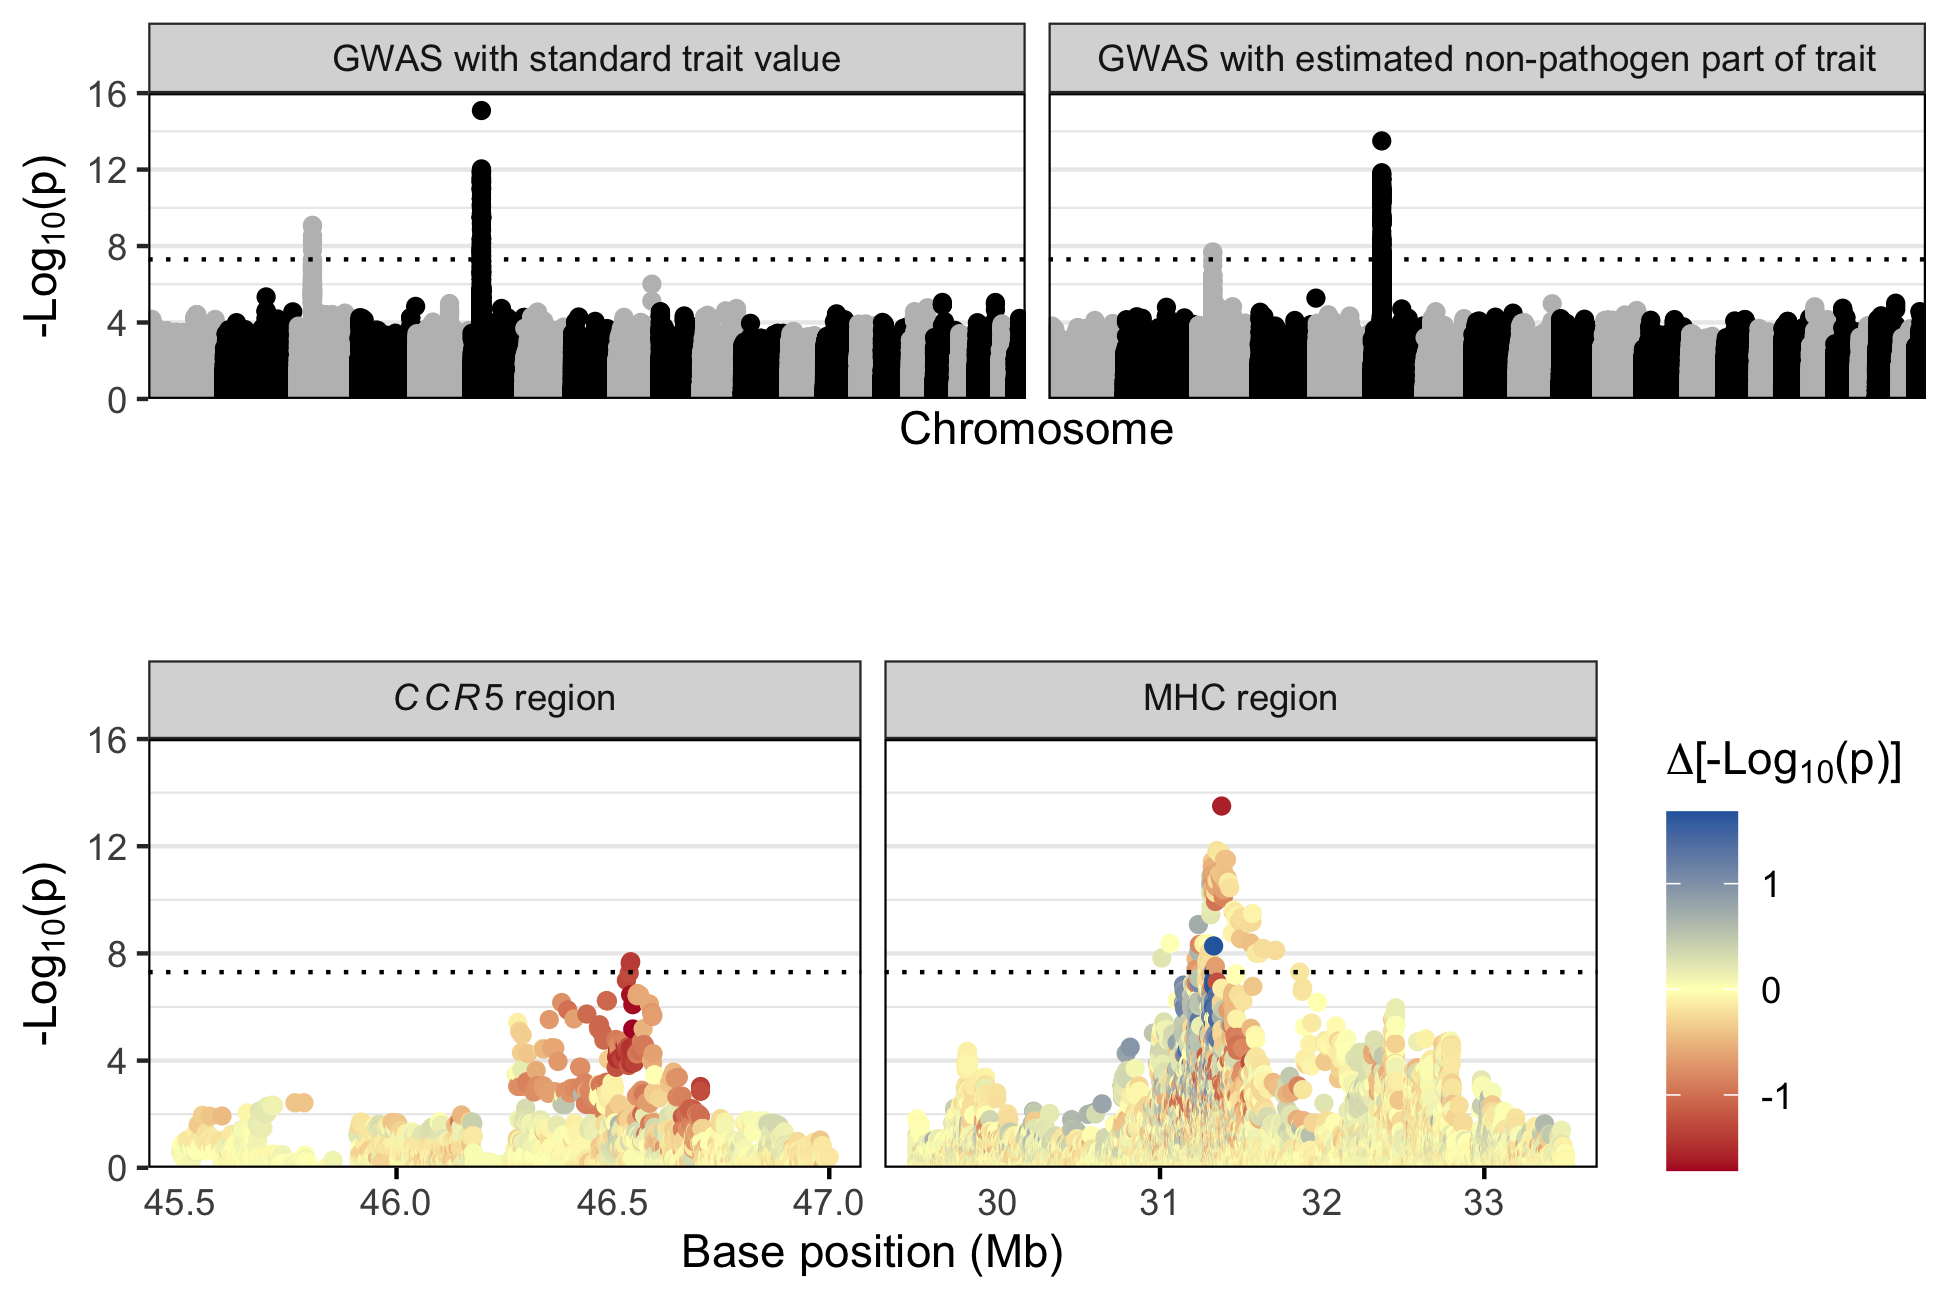
\includegraphics[width=\linewidth]{figures/gwas_results}
		\caption{Results from comparative \DIFaddbeginFL \DIFaddFL{genome-wide association studies (}\DIFaddendFL GWAS\DIFaddbeginFL \DIFaddFL{) on HIV-1 set-point viral load (spVL) data}\DIFaddendFL . (A) shows association p-values for the same host variants from the \DIFdelbeginFL \DIFdelFL{SHCS }\DIFdelendFL \DIFaddbeginFL \DIFaddFL{Swiss HIV }\DIFaddendFL cohort in GWAS with two different response variables. On the left, we used unmodified \DIFaddbeginFL \DIFaddFL{(total) }\DIFaddendFL spVL values. On the right, we used our estimates for the non-pathogen effects on spVL. The alternating shades correspond to different chromosomes. (B) compares the strength of association for variants in the \emph{CCR5} and MHC regions between the two GWAS (positions 45.4 - 47Mb on chromosome 3 and 29.5 - 33.5Mb on chromosome 6 for the \emph{CCR5} and MHC, respectively). Base positions are with reference to genome build GRCh37. The color of each point represents the difference in -log$_{10}$ p-value between the two GWAS. Red means taking into account phylogenetic information decreased the strength of association and blue means it increased it. The dashed lines show genome-wide significance at p = \DIFdelbeginFL \DIFdelFL{5x10$^{-8}$}\DIFdelendFL \DIFaddbeginFL \DIFaddFL{$5 \times 10^{-8}$}\DIFaddendFL .}
		\label{fig:gwas-results}
	\end{center}
\end{figure}

\begin{table}[H]
\centering
\caption{Top association results from \citet{McLaren2015} compared to results from this study. \DIFdelbeginFL \DIFdelFL{The }\DIFdelendFL \DIFaddbeginFL \DIFaddFL{Results from this study are for host variants from the SHCS in GWAS with two different response variables. }\DIFaddendFL ``Standard trait value'' \DIFaddbeginFL \DIFaddFL{means we used the unmodified (total) spVL value }\DIFaddendFL and ``Estimated non-pathogen part of trait'' \DIFdelbeginFL \DIFdelFL{results are from using two different GWAS response variables with }\DIFdelendFL \DIFaddbeginFL \DIFaddFL{means we used our estimates for }\DIFaddendFL the \DIFdelbeginFL \DIFdelFL{same human genotype data}\DIFdelendFL \DIFaddbeginFL \DIFaddFL{non-pathogen effects on spVL}\DIFaddendFL .}
\begin{tabularx}{\linewidth}{p{1cm}p{1.8cm}p{2.4cm}p{1.8cm}p{2cm}p{1.8cm}p{2cm}} % {lrrrrrr} {llclcccc}
\hline
& & \makecell{McLaren \\ et al.}  & \multicolumn{2}{l}{\makecell{Standard \\ trait value}} & \multicolumn{2}{l}{\makecell{Estimated non-pathogen \\ part of trait}} \\ 
  \hline
 Region & Variant & p-value & Effect size & p-value & Effect size & p-value \\
  \hline
    MHC & rs59440261 & $2.0 \times 10^{-83}$ & -0.4 & $3.3 \times 10^{-11}$ & -0.22 & $2.6 \times 10^{-10}$ \\ 
    \emph{CCR5} & rs1015164 & $1.5 \times 10^{-19}$ & 0.15 & $7.5 \times 10^{-7}$ & 0.078 & $8.5 \times 10^{-6}$ \\ 
   \hline
\end{tabularx}
\label{tab:comp-gwas-mclaren-snps}
\end{table}

\DIFaddbegin \subsection*{\DIFadd{Application to the }\emph{\DIFadd{A. thaliana}}\DIFadd{-}\emph{\DIFadd{X. arboricola}} \DIFadd{pathosystem}}

\DIFadd{Next, we applied our method to data collected from the }\emph{\DIFadd{A. thaliana}}\DIFadd{-}\emph{\DIFadd{X. arboricola}} \DIFadd{pathosystem by \mbox{%DIFAUXCMD
\cite{Wang2018Two-wayGenomes}}\hskip0pt%DIFAUXCMD
. \mbox{%DIFAUXCMD
\cite{Wang2018Two-wayGenomes} }\hskip0pt%DIFAUXCMD
performed a fully-crossed experiment in which they infected genetically diverse }\emph{\DIFadd{A. thaliana}} \DIFadd{accessions with genetically diverse strains of the phytopathogenic bacteria }\emph{\DIFadd{X. arboricola}}\DIFadd{. They scored quantitative disease resistance (QDR) on a scale of 0 (resistant) to 4 (susceptible) for up to four infected leaves for three replicates of each }\emph{\DIFadd{A. thaliana}}\DIFadd{-}\emph{\DIFadd{X. arboricola}} \DIFadd{pairing. Our method requires a single trait value per pathogen strain, so we used mean QDR calculated for each pathogen strain across all the host }\emph{\DIFadd{A. thaliana}} \DIFadd{types (Figure \ref{fig:application-exp-setup}B). Figure \ref{fig:qdr-on-tree}A shows the inferred }\emph{\DIFadd{X. arboricola}} \DIFadd{pathogen phylogeny annotated with the  mean QDR trait value used for each strain. Mean QDR  was generally low, varying between 0.11 for strain NL\_P126 and 0.78 for strain FOR\_F21. Fitting the POUMM yielded very low selection strength $\alpha$ and intensity of stochastic fluctuations  $\sigma$ parameter estimates (posterior mean 0.03 with 95\% HPD 0.0 - 0.05 and 0.03 with 95\% HPD 0.0 - 0.06, respectively; Table \ref{tab:POUMM-parameters-our-estimates-qdr}). These values deviated significantly from the respective priors (Figure \ref{fig:poumm-parameters-qdr}). Heritability, on the other hand, was quite uncertain (posterior mean 0.33 with 95\% HPD 0.0 - 0.77; Table \ref{tab:POUMM-parameters-our-estimates-qdr}). The posterior mean selection strength and heritability values are also shown in the context of the simulation study as points on Figure \ref{fig:simulationResults}.
}

\DIFadd{Given the posterior mean estimates for the POUMM parameters, expected correlation in trait values between tips were very low (maximum value $3.2 \times 10^{-12}$ compared to maximum value of 0.45 in the HIV-1 spVL application). Thus, the phylogeny is not very informative for a trait value correction. Indeed, the estimated pathogen part of the QDR trait calculated by our method is simply a scaling of the total QDR trait value (Figure \ref{fig:trait-comparison-qdr}). We anyways selected 22 random host-pathogen strain pairings to perform a comparative GWAS analogous to that for HIV-1 spVL, where each host is infected with a single pathogen strain. In the first GWAS, we used the specific QDR measurement for each selected host-pathogen pairing. I.e., with reference to Figure \ref{fig:application-exp-setup}, we selected $z_{11}$ for the first sample, $z_{23}$ for the second sample, and so on. In the second GWAS, we used our estimates for the non-pathogen effects on QDR for each pairing. Since our method did not utilize phylogenetic information in this case, the estimated non-pathogen part of the trait is simply the specific QDR for each selected host-pathogen pairing, minus mean QDR for the respective pathogen strain, calculated across all the host }\emph{\DIFadd{A. thaliana}} \DIFadd{types. I.e., with reference to Figure \ref{fig:application-exp-setup}, we used a scaled version of $z_{11} - \bar{z}_1$ for the first sample, $z_{23} - \bar{z}_2$ for the first sample, and so on. Figure \ref{fig:gwas-results-qdr} shows that results are qualitatively similar between the two GWAS, with a slight decrease in association strength for the top-associated variants. Q-Q plots show the distribution of p-values are also very similar (Figure \ref{fig:qq-plots-qdr}). In the first, standard GWAS, one }\emph{\DIFadd{A. thaliana}} \DIFadd{loci just exceeds the threshold for significant association after correction for multiple testing. In the second, corrected GWAS, no }\emph{\DIFadd{A. thaliana}} \DIFadd{variants are significantly associated with QDR to }\emph{\DIFadd{X. arboricola}}\DIFadd{.
}

\begin{figure}[H]
\begin{center}
    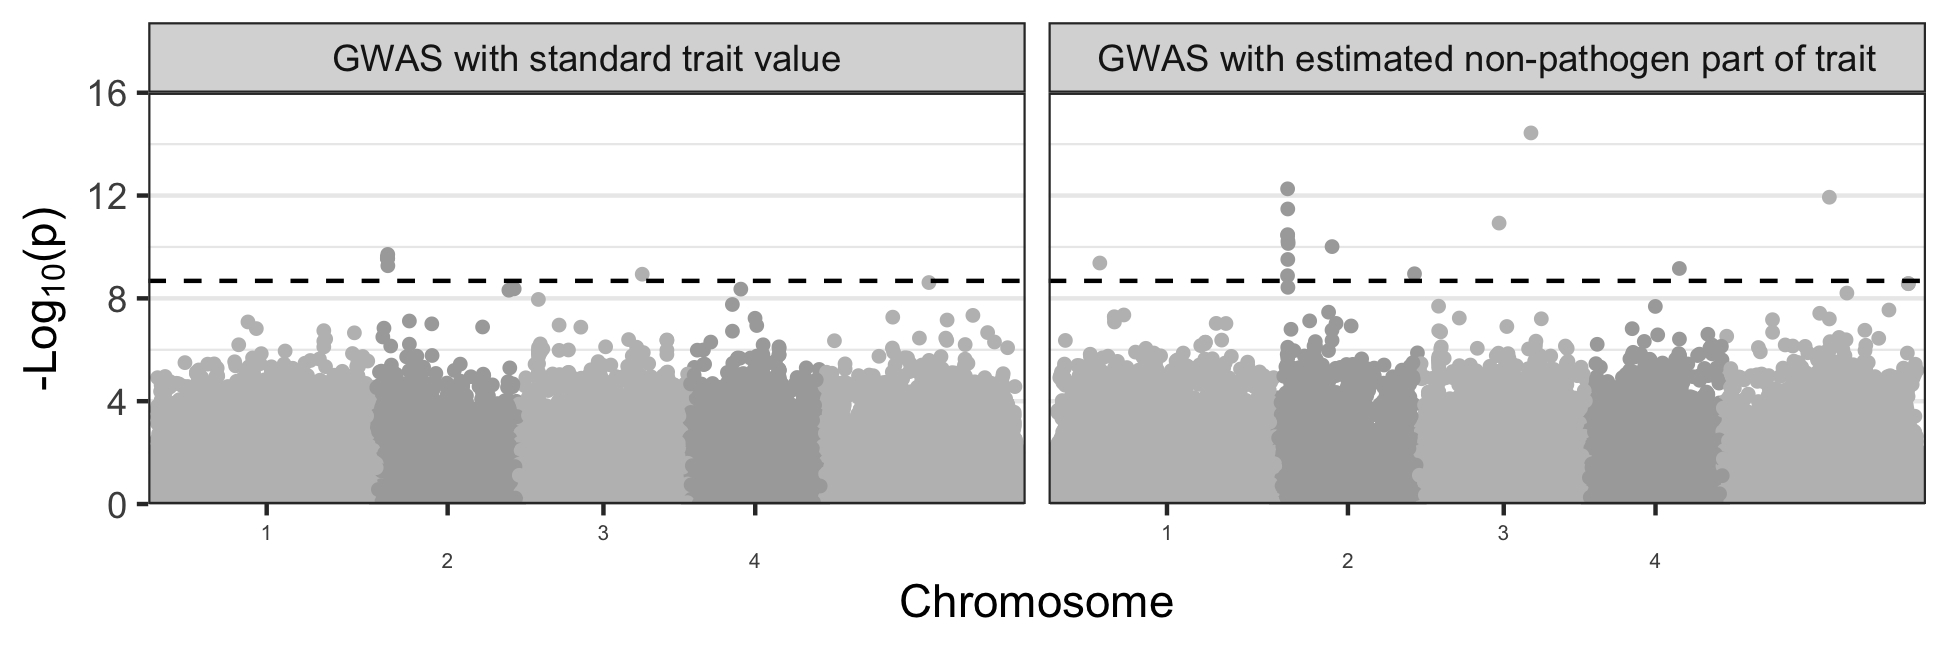
\includegraphics[width = \linewidth]{figures/gwas_results_xanthomonas}
	\caption{\DIFaddFL{Results from comparative genome-wide association studies (GWAS) on }\emph{\DIFaddFL{A. thaliana}} \DIFaddFL{quantitative disease resistance (QDR) to }\emph{\DIFaddFL{X. arboricola}}\DIFaddFL{. The two facets show association p-values for the same host }\emph{\DIFaddFL{A. thaliana}} \DIFaddFL{variants in GWAS with two different response variables. On the left, we used unmodified (total) QDR values for each of the 22 selected host-pathogen pairings on which these results are based. On the right, we used our estimates for the non-pathogen effects on QDR for these samples. In this case, estimated non-pathogen effects are the specific QDR for each selected host-pathogen pairing, minus mean QDR for the respective pathogen strain, calculated across all the host }\emph{\DIFaddFL{A. thaliana}} \DIFaddFL{types. The alternating shades correspond to different chromosomes. The dashed lines show significance at significance level 0.05 with a Bonferroni correction for multiple testing.}}
	\label{fig:gwas-results-qdr}
	\end{center}
\end{figure}

\DIFaddend \section*{Discussion}
% State the importance of your findings
In this paper, we presented a \DIFdelbegin \DIFdel{novel, }\DIFdelend \DIFaddbegin \DIFadd{new }\DIFaddend phylogeny-aware GWAS framework to correct for heritable pathogen effects on infectious disease traits. By using information from the pathogen phylogeny, we show \DIFaddbegin \DIFadd{that }\DIFaddend it is possible to improve GWAS power to detect host genetic variants associated with a disease trait. This \DIFdelbegin \DIFdel{should help us better understand }\DIFdelend \DIFaddbegin \DIFadd{improved power is envisioned to contribute to a better understanding of }\DIFaddend which host factors are \DIFaddbegin \DIFadd{broadly }\DIFaddend protective against a disease versus which increase susceptibility or disease severity.

% Contextualize the study & address limitations
\DIFdelbegin \DIFdel{Our method relies on the POUMM, a model of continuous trait evolution that accounts for heritable and non-heritable effects on a trait, as well as selection . Using this model , we }\DIFdelend \DIFaddbegin \DIFadd{The main novelty of our approach is to estimate parameters governing the evolutionary dynamics of a trait in the pathogen population and use these estimates to correct infectious disease trait values prior to performing GWAS, thereby estimating and removing pathogen effects. In simulations, we show that when trait heritability due to shared pathogen ancestry amongst infection partners is greater than approximately 25\%, GWAS power to detect host genetic variants associated with the same trait is reduced. Our method can correct for this effect in certain evolutionary scenarios by using information from the full pathogen phylogeny. Based on our simulation results, our method is anticipated to be very useful for disease traits that are highly heritable from donor to recipient and  maintain a high correlation between sampled individuals. In simulations, we showed this is the case when pathogen heritability is high, selection strength is low, and trait values are not subject to strong stochastic fluctuations. In summary, cohort-level, phylogenetically structured differences in the measured trait value are necessary for our approach to outperform state of the art methods. 
}

\DIFadd{We applied this model to two different host-pathogen systems where paired host and pathogen genetic data was generated alongside a measure of pathogen virulence. First, we fit the POUMM to set-point viral load data from individuals living with HIV in Switzerland. We }\DIFaddend estimated HIV-1 spVL heritability to be 45\% (95\% HPD 24 - 67\%) in \DIFdelbegin \DIFdel{the Swiss HIV Cohort Study}\DIFdelend \DIFaddbegin \DIFadd{this cohort}\DIFaddend . Compared to previous studies, this estimate is at the higher end \DIFdelbegin \DIFdel{\mbox{%DIFAUXCMD
\citep{Mitov2018}}\hskip0pt%DIFAUXCMD
}\DIFdelend \DIFaddbegin \DIFadd{(see \mbox{%DIFAUXCMD
\citet{Mitov2018} }\hskip0pt%DIFAUXCMD
and references therein)}\DIFaddend . Also using the POUMM, \DIFdelbegin \DIFdel{\mbox{%DIFAUXCMD
\citep{Bertels2018} }\hskip0pt%DIFAUXCMD
}\DIFdelend \DIFaddbegin \DIFadd{\mbox{%DIFAUXCMD
\citet{Bertels2018} }\hskip0pt%DIFAUXCMD
}\DIFaddend estimated a spVL heritability of 29\% (N = 2014, CI 12 - 46\%) from the same cohort and \DIFdelbegin \DIFdel{\mbox{%DIFAUXCMD
\citep{Blanquart2017} }\hskip0pt%DIFAUXCMD
}\DIFdelend \DIFaddbegin \DIFadd{\mbox{%DIFAUXCMD
\citet{Blanquart2017} }\hskip0pt%DIFAUXCMD
}\DIFaddend estimated 31\% (N = 2028, CI 15 - 43\%) from a pan-European cohort. We note that our sample size (N = 1493 individuals) is smaller than in these other studies. This might be because we restricted samples based on having $pol$ gene sequences with at least 750 non-ambiguous bases. Our aim was to reconstruct a high-quality phylogeny, since the POUMM does not account for phylogenetic uncertainty and the POUMM parameter estimates are key to our downstream \DIFdelbegin \DIFdel{GWAS methods}\DIFdelend \DIFaddbegin \DIFadd{trait-correction method}\DIFaddend . Although our heritability estimate is rather high, the confidence interval largely overlaps \DIFdelbegin \DIFdel{that }\DIFdelend \DIFaddbegin \DIFadd{with the intervals  }\DIFaddend of other studies and we note that estimating heritability per se was not our primary focus.

\DIFdelbegin \DIFdel{Instead, }\DIFdelend \DIFaddbegin \DIFadd{For comparison, we also fit the POUMM to quantitative disease resistance measurements from }\emph{\DIFadd{A. thaliana}} \DIFadd{infected with the phytopathogenic bacteria }\emph{\DIFadd{X. arboricola}}\DIFadd{. We estimated }\emph{\DIFadd{X. arboricola}} \DIFadd{virulence heritability to be 33\% (95\% HPD 0 - 77\%). \mbox{%DIFAUXCMD
\citep{Wang2018Two-wayGenomes} }\hskip0pt%DIFAUXCMD
originally estimated a QDR heritability of 44\% in this dataset, falling within the wide range of our estimate. We note that \mbox{%DIFAUXCMD
\cite{Wang2018Two-wayGenomes} }\hskip0pt%DIFAUXCMD
used a linear mixed model in which the experimental unit is QDR scored on individual leaves, whereas our estimate is based on much coarser binning of QDR scores into a mean score across all leaves on all host accessions and all replicates (N = 22). Furthermore, }\DIFaddend the \DIFdelbegin \DIFdel{main novelty of our approach was to correct the spVL trait prior to performing the GWAS, thereby estimating and removing pathogen effects. In simulations, we show that when trait heritability amongst infection partners is greater than approximately 25\% , GWAS power to detect host genetic variants associated with the same trait is reduced. Our method can correct for this effect in certain evolutionary scenarios by using information from the full pathogen phylogeny. 
}%DIFDELCMD < 

%DIFDELCMD < %%%
\DIFdel{Based on our simulation results, our method is anticipated to be very useful for disease traits that are highly heritable from donor to recipient and  maintain a high correlation between sampled individuals. In simulations, we showed this is the case when heritability is high, selection strength is low, and trait values are not subject to strong stochastic fluctuations. So, cohort-level, phylogenetically structured differences in the measured trait value are necessary for our approach to outperform state of the art methods}\DIFdelend \DIFaddbegin \DIFadd{QDR score trait values were not truly continuous (scores were measured on an integer scale from 0 to 4). Thus, these data partially violate the assumptions of the POUMM. We estimate very low selection strength for virulence in }\emph{\DIFadd{X. arboricola}}\DIFadd{. As \mbox{%DIFAUXCMD
\cite{Wang2018Two-wayGenomes} }\hskip0pt%DIFAUXCMD
explain, }\emph{\DIFadd{X. arboricola}} \DIFadd{strains with differing virulence can co-inhabit populations of }\emph{\DIFadd{A. thaliana}}\DIFadd{. This might also point to low selection on }\emph{\DIFadd{X. arboricola}} \DIFadd{virulence. Furthermore, expected correlation in virulence between related strains of }\emph{\DIFadd{X. arboricola}} \DIFadd{was smaller than for HIV-1}\DIFaddend .

Given our estimates for \DIFdelbegin \DIFdel{the heritability of spVL and the }\DIFdelend \DIFaddbegin \DIFadd{trait heritability and }\DIFaddend selection strength on \DIFdelbegin \DIFdel{this trait using Swiss HIV cohort data}\DIFdelend \DIFaddbegin \DIFadd{HIV-1 spVL and }\emph{\DIFadd{A. thaliana}} \DIFadd{QDR to }\emph{\DIFadd{X. arboricola}}\DIFaddend , our simulation results reveal that we cannot expect a significant improvement in GWAS power for \DIFdelbegin \DIFdel{human genetic determinants of spVL }\DIFdelend \DIFaddbegin \DIFadd{these systems }\DIFaddend (Figure \ref{fig:simulationResults}). Indeed\DIFdelbegin \DIFdel{the results of our  GWAS method presented here and a standard GWAS are very similar. Future applications might investigate other clinically significant disease traits and outcomes that are affected by both host and pathogen genetic factors, for instance Hepatitis B Virus-related hepatocellular carcinoma \mbox{%DIFAUXCMD
\citep{An2018HostCarcinoma}}\hskip0pt%DIFAUXCMD
, Hepatitis C treatment success \mbox{%DIFAUXCMD
\citep{Ansari2017Genome-to-genomeVirus}}\hskip0pt%DIFAUXCMD
, and susceptibility to or severity of certain bacterial infections, e. g. \mbox{%DIFAUXCMD
\cite{Messina2016ImpactInfections, Donnenberg2015BacterialStudies}}\hskip0pt%DIFAUXCMD
. }\DIFdelend \DIFaddbegin \DIFadd{, while certain pairs of samples in the HIV-1 cohort were expected to have phylogenetically correlated spvL values (maximum expected correlation between any two samples was 0.45), the overall effect on GWAS is small. For HIV-1 spVL, our phylogenetic correction slightly decreases p-values for variants in $CCR5$ and slightly decreases some and increases other p-values for variants in the MHC (Figure \ref{fig:gwas-results}B). Simulations show we shouldn't expect a net p-value decrease, but our simulations represent an ideal scenario since we simulate under the POUMM. For the empirical data, un-modeled evolutionary pressures like drug treatment and host-specific HLA alleles might cause the reduced p-values. However, the overall picture is consistent between the two GWAS (Figure \ref{fig:gwas-results}A). For }\emph{\DIFadd{A. thaliana}} \DIFadd{QDR to }\emph{\DIFadd{X. arboricola}}\DIFadd{, the trait value correction does not utilize phylogenetic information because phylogenetic correlations between samples are too weak (maximum expected correlation between strains was $3.2 \times 10^{-12}$). We anyways corrected QDR trait values based on average QDR for each pathogen strain across the full range of host types. Results show slight decrease in p-values for the most-associated variants in this application as well, but the overall picture is consistent with previous GWAS results from \mbox{%DIFAUXCMD
\cite{Wang2018Two-wayGenomes}}\hskip0pt%DIFAUXCMD
. That study found no significant }\emph{\DIFadd{A. thaliana}} \DIFadd{variants associated with QDR using a linear mixed model jointly accounting for host genetic effects, pathogen genetic effects, and interaction effects. As with HIV-1 spVL, our results do not challenge this previous finding. Therefore, we conclude that GWAS for host determinants of HIV-1 subtype B spVL and }\emph{\DIFadd{A. thaliana}} \DIFadd{determinants of QDR to }\emph{\DIFadd{X. arboricola}} \DIFadd{are robust to our correction for pathogen effects.
}\DIFaddend 

\DIFdelbegin \DIFdel{Our method is convenient for GWAS because it is simply a }\DIFdelend \DIFaddbegin \DIFadd{Our method has several limitations. When POUMM parameter estimates are highly uncertain, correcting trait values based on posterior mean or maximum likelihood parameter estimates neglects this uncertainty. Then, as in the }\emph{\DIFadd{A. thaliana}}\DIFadd{-}\emph{\DIFadd{X. arboricola}} \DIFadd{application, fitting the POUMM may reveal that expected phylogenetic correlations between samples are not strong enough to justify using our method to correct trait values in a GWAS. In this case, one may wish to use a linear mixed model as in \mbox{%DIFAUXCMD
\cite{Wang2018Two-wayGenomes}}\hskip0pt%DIFAUXCMD
, where the pathogen effect is co-estimated as a random effect. The expected correlation structure estimated under the POUMM could be used for the covariance of the random effect, taking the phylogeny into account differently but still utilizing information from the evolutionary model. Finally, as we show here, our method is not anticipated to be useful in certain evolutionary scenarios. For instance, traits like antimicrobial resistance may be under strong selection pressure and be highly heritable. In these instances, our simulations do not point to a large improvement when adding our }\DIFaddend pre-processing \DIFaddbegin \DIFadd{step. In any case, such traits might violate the POUMM assumption that trait values vary as a random walk in continuous space if they are caused by few mutations of strong affect, meaning our approach would not apply. In this situation, one would rather account for antimicrobial resistance as a covariate in the GWAS association model.
}

\DIFadd{The primary advantage of our approach is that it is complementary to previously developed methods for infectious disease GWAS. First, it provides additional information on the evolutionary dynamics of the trait in the pathogen population. Then, it is a convenient pre-processing }\DIFaddend step \DIFdelbegin \DIFdel{that produces an alternate }\DIFdelend \DIFaddbegin \DIFadd{for GWAS because it simply produces a corrected }\DIFaddend response variable for GWAS association tests.  \DIFdelbegin \DIFdel{Therefore, it is still possible to use previously developed , well-documented, and fast tools }\DIFdelend \DIFaddbegin \DIFadd{In cases where a correction can be estimated and applied using our method, the corrected trait values are envisioned to be used in any of the previously developed GWAS models }\DIFaddend for the actual association testing (we used \DIFdelbegin \DIFdel{PLINK \mbox{%DIFAUXCMD
\citep{Chang2015}}\hskip0pt%DIFAUXCMD
). The method }\DIFdelend \DIFaddbegin \DIFadd{a linear model approach implemented in PLINK \mbox{%DIFAUXCMD
\citep{Chang2015}}\hskip0pt%DIFAUXCMD
, though a more advanced method would be to use a linear mixed model with host ancestry as a random effect). Further, additional model complexity can be added to the GWAS association tests. For instance, our method does not account for co-infection, which might add additional variance to trait values and decrease GWAS power. In this case, one could add co-infection status as a covariate in the GWAS association test to account for this variable. 
}

\DIFadd{Our method }\DIFaddend relies on the freely available R package POUMM \citep{Mitov2017a-POUMM}\DIFdelbegin \DIFdel{and all the code we wrote }\DIFdelend \DIFaddbegin \DIFadd{, which scales to trees of up to 10,000 tips \mbox{%DIFAUXCMD
\citep{Mitov2019}}\hskip0pt%DIFAUXCMD
. All code for the simulations and HIV spVL analysis presented in this study }\DIFaddend is available on the project GitHub at https://github.com/cevo-public/POUMM-GWAS. \DIFaddbegin \DIFadd{Future applications of our method might investigate other clinically significant disease traits and outcomes that are affected by both host and pathogen genetic factors, for instance Hepatitis B Virus-related hepatocellular carcinoma \mbox{%DIFAUXCMD
\citep{An2018HostCarcinoma}}\hskip0pt%DIFAUXCMD
, Hepatitis C treatment success \mbox{%DIFAUXCMD
\citep{Ansari2017Genome-to-genomeVirus}}\hskip0pt%DIFAUXCMD
, and susceptibility to or severity of certain bacterial infections, e.g. \mbox{%DIFAUXCMD
\cite{Messina2016ImpactInfections, Donnenberg2015BacterialStudies}}\hskip0pt%DIFAUXCMD
. Transcriptomic data has also previously been modeled as an evolving phenotype using an Ornstein-Uhlenbeck model \mbox{%DIFAUXCMD
\citep{Rohlfs2014ModelingVariation}}\hskip0pt%DIFAUXCMD
. Thus, one could also estimate pathogen effects on host gene expression.
}\DIFaddend 

% Summarize the paper
In summary, we \DIFdelbegin \DIFdel{argue that }\DIFdelend \DIFaddbegin \DIFadd{present a coherent }\DIFaddend infectious disease GWAS \DIFdelbegin \DIFdel{should take }\DIFdelend \DIFaddbegin \DIFadd{framework that takes }\DIFaddend the pathogen phylogeny into account when searching for host determinants of a disease trait. We \DIFdelbegin \DIFdel{give a practical threshold for identifying when GWAS suffer from pathogen effects (}\DIFdelend \DIFaddbegin \DIFadd{further show that the pathogen phylogeny only has an impact on the GWAS outputs if }\DIFaddend heritability of the trait amongst infection partners \DIFaddbegin \DIFadd{is }\DIFaddend $>$ 25\%\DIFdelbegin \DIFdel{) and provide a method that can help in scenarios where trait values are highly heritable and phylogenetically-structured amongst members of a cohort}\DIFdelend \DIFaddbegin \DIFadd{.
For the systems studied here, spVL in individuals living with HIV and QDR for X. arboricola infections in A. thaliana, the phylogenetic correction does not change GWAS results. Our findings indicate previously published GWAS results for these systems are not biased by shared evolutionary history amongst infecting pathogen strains}\DIFaddend .

\section*{Materials and Methods}

\subsection*{Simulation model}

Whenever possible, we tried to parameterize our simulation model \DIFdelbegin \DIFdel{for spVL }\DIFdelend using empirical data \DIFaddbegin \DIFadd{on the spVL trait}\DIFaddend . We set the total variance in spVL to 0.73 log copies$^2$ mL$^{-2}$ based on UK cohort data \citep{Mitov2018}. \DIFaddbegin \DIFadd{Other studies have estimated slightly lower values though (Table \ref{tab:spVLmeasurements}). }\DIFaddend After allotting 25\% of this variance to \DIFdelbegin \DIFdel{the }\DIFdelend \DIFaddbegin \DIFadd{a }\DIFaddend host part of spVL \DIFdelbegin \DIFdel{$g_h$ (following \mbox{%DIFAUXCMD
\citet{McLaren2015}}\hskip0pt%DIFAUXCMD
)}\DIFdelend \DIFaddbegin \DIFadd{$h$ based on results by \mbox{%DIFAUXCMD
\citet{McLaren2015}}\hskip0pt%DIFAUXCMD
}\DIFaddend , we partitioned the remaining variance between \DIFdelbegin \DIFdel{the viral part $g_v$ and the environmental part $\epsilon$ }\DIFdelend \DIFaddbegin \DIFadd{a viral part $g$ and an environmental part $e$ }\DIFaddend in different ratios to assess estimator performance across a range of spVL heritabilities. \DIFdelbegin \DIFdel{$g_h$ }\DIFdelend \DIFaddbegin \DIFadd{$h$ }\DIFaddend was simulated as the sum of contributions from 20 causal host genetic variants, 10 of which had an effect size of 0.2 log copies mL$^{-1}$ and 10 of which had an effect size of -0.2 log copies mL$^{-1}$. Host genetic variants were generated from a binomial distribution with probability $p$ calculated such that \DIFdelbegin \DIFdel{$g_h$ }\DIFdelend \DIFaddbegin \DIFadd{$h$ }\DIFaddend had the appropriate variance (see Table \ref{tab:sim-params}). We generated a random viral phylogeny with branch lengths on the same time scale as a previously inferred UK cohort HIV tree \citep{Hodcroft2014} using the R package ape \citep{Paradis2018}. \DIFdelbegin \DIFdel{$g_v$ }\DIFdelend \DIFaddbegin \DIFadd{$g$ }\DIFaddend was simulated by running an OU process along the phylogeny using the R package POUMM \citep{Mitov2017a-POUMM} and sampling values at the tips. For the OU parameters $\theta$ and $g_{0}$ we used 4.5 log copies mL$^{-1}$ \DIFdelbegin \DIFdel{, }\DIFdelend \DIFaddbegin \DIFadd{based on previous estimates of mean spVL (Table \ref{tab:spVLmeasurements}). This is }\DIFaddend similar to values previously inferred for HIV (Table \DIFdelbegin \DIFdel{\ref{tab:POUMM-parameters-our-estimates}}\DIFdelend \DIFaddbegin \DIFadd{\ref{tab:POUMMparams-prev-estimated}}\DIFaddend ). To assess our estimator's performance under a range of evolutionary scenarios, we co-varied the \DIFdelbegin \DIFdel{OU parameters for selection strength , }\DIFdelend \DIFaddbegin \DIFadd{heritability $H^2$ and selection strength }\DIFaddend $\alpha$ \DIFdelbegin \DIFdel{, and }\DIFdelend \DIFaddbegin \DIFadd{parameters. The }\DIFaddend intensity of random fluctuations \DIFdelbegin \DIFdel{, }\DIFdelend $\sigma$ \DIFdelbegin \DIFdel{, so that different proportions of the variability in $g_v$ were attributable to selection and drift, respectively}\DIFdelend \DIFaddbegin \DIFadd{was determined based on these parameters (Table \ref{tab:sim-params}, Figure \ref{fig:sigma-vs-alpha})}\DIFaddend . Finally, the environmental \DIFdelbegin \DIFdel{component of spVL $\epsilon$ }\DIFdelend \DIFaddbegin \DIFadd{part of spVL $e$ }\DIFaddend was generated from a normal distribution with mean 0.  For a full graphical model representation of the simulation scheme, see Figure \ref{fig:sim-design}. 

\DIFdelbegin %DIFDELCMD < \begin{table}[H]
%DIFDELCMD < 	%%%
%DIFDELCMD < \caption{%
{%DIFAUXCMD
\DIFdelFL{Simulation model parameters. For a full graphical model representation of the simulation scheme, including how these parameters are related, see Figure \ref{fig:sim-design}.}}
	%DIFAUXCMD
%DIFDELCMD < \begin{tabularx}{\linewidth}{p{1.5cm}ll} \toprule 
%DIFDELCMD < 		%%%
\DIFdelFL{Variable }%DIFDELCMD < & %%%
\DIFdelFL{Expression }%DIFDELCMD < & %%%
\DIFdelFL{Definition }%DIFDELCMD < \\ \midrule 
%DIFDELCMD < 		%%%
\DIFdelFL{$\sigma^2_z$ }%DIFDELCMD < &  %%%
\DIFdelFL{0.73 log copies$^{2}$/mL$^{2}$ }%DIFDELCMD < & %%%
\DIFdelFL{Total spVL variance }%DIFDELCMD < \\ 
%DIFDELCMD < 		%%%
\DIFdelFL{$H^2_h$ }%DIFDELCMD < & %%%
\DIFdelFL{0.25 }%DIFDELCMD < & %%%
\DIFdelFL{Host heritability of spVL }%DIFDELCMD < \\
%DIFDELCMD < 		%%%
\DIFdelFL{$H^2_{\bar{t}}$ }%DIFDELCMD < & %%%
\DIFdelFL{varied }%DIFDELCMD < & %%%
\DIFdelFL{Viral heritability of spVL at $\bar{t}$ }%DIFDELCMD < \\
%DIFDELCMD < 		%%%
\DIFdelFL{$\sigma^2_{g_h}$ }%DIFDELCMD < & %%%
\DIFdelFL{$\sigma_{g_h}^2 = 0.25*\sigma_z^2$ }%DIFDELCMD < & %%%
\DIFdelFL{Variance in host part of spVL }%DIFDELCMD < \\
%DIFDELCMD < 		%%%
\DIFdelFL{$\sigma^2_{g_v}(\bar{t})$ }%DIFDELCMD < & %%%
\DIFdelFL{$\sigma^2_{g_{v}}(\bar{t}) = H^2_{\bar{t}}*\sigma_z^2$ }%DIFDELCMD < & %%%
\DIFdelFL{Variance in viral part of spVL at $\bar{t}$ }%DIFDELCMD < \\ 
%DIFDELCMD < 		%%%
\DIFdelFL{$\sigma^2_{\epsilon}$ }%DIFDELCMD < & %%%
\DIFdelFL{$\sigma_{\epsilon}^2 = \sigma_z^2 - \sigma^2_{g_v} - \sigma^2_{g_h}$ }%DIFDELCMD < & %%%
\DIFdelFL{Variance in environmental part of spVL }%DIFDELCMD < \\ 
%DIFDELCMD < 		%%%
\DIFdelFL{$\bar{t}$ }%DIFDELCMD < & %%%
\DIFdelFL{0.14 substitutions site$^{-1}$ yr$^{-1}$ }%DIFDELCMD < & %%%
\DIFdelFL{Mean root-tip time in viral phylogeny }%DIFDELCMD < \\ 
%DIFDELCMD < 		%%%
\DIFdelFL{$\bm{g}_v$ }%DIFDELCMD < & %%%
\DIFdelFL{$\bm{g}_v \sim Norm(\bm{\mu}_{OU}, \boldsymbol{\Sigma}_{OU})$ }%DIFDELCMD < & %%%
\DIFdelFL{Viral part of spVL for all individuals }%DIFDELCMD < \\ 
%DIFDELCMD < 		%%%
\DIFdelFL{$\theta$ }%DIFDELCMD < & %%%
\DIFdelFL{4.5 log copies/mL }%DIFDELCMD < & %%%
\DIFdelFL{Optimal spVL value}%DIFDELCMD < \\
%DIFDELCMD < 		%%%
\DIFdelFL{$g_{0}$ }%DIFDELCMD < & %%%
\DIFdelFL{4.5 log copies/mL }%DIFDELCMD < & %%%
\DIFdelFL{$g_v$ at the root of the phylogeny  }%DIFDELCMD < \\ 
%DIFDELCMD < 		%%%
\DIFdelendFL \DIFaddbeginFL \DIFaddFL{We performed GWAS on the simulated data using a linear association model as implemented in the ``lm'' function in R. For each simulated dataset, we performed three association tests: (i) using the true (simulated) non-pathogen part of the trait (host + environmental parts), (ii) using the estimated non-pathogen part of the trait according to the method presented in this paper, and (iii) using the total trait value, scaled by its mean. We assessed the significance of each associations at a significance level of 0.05 with a Bonferroni correction for multiple testing. For our main results (Figure \ref{fig:simulationResults}) we simulated 20 truly associated variants, as described above. To also check the false positive rate (FPR), we re-ran the simulations with an additional 80 non-associated variants. Across all the association tests in this second simulation setup (7 $H^2$ levels $\times$ 10 }\DIFaddendFL $\alpha$ \DIFdelbeginFL %DIFDELCMD < & %%%
\DIFdelFL{varied }%DIFDELCMD < & %%%
\DIFdelFL{Selection strength of OU process }%DIFDELCMD < \\ 
%DIFDELCMD < 		%%%
\DIFdelFL{$\sigma$ }%DIFDELCMD < & %%%
\DIFdelFL{$\sigma = \sqrt{\frac{2\alpha\sigma^2_{g_{v}}(\bar{t})}{1 - exp(-2\alpha\bar{t})}}$ }%DIFDELCMD < & %%%
\DIFdelFL{Time-unit standard deviation of OU process }%DIFDELCMD < \\ 
%DIFDELCMD < 		%%%
\DIFdelFL{$\Psi$ }%DIFDELCMD < & %%%
\DIFdelFL{branch lengths $\sim Exp(\bar{t})$ }%DIFDELCMD < & %%%
\DIFdelFL{Viral phylogeny }%DIFDELCMD < \\ 
%DIFDELCMD < 		%%%
\DIFdelFL{$g_{h_i}$ }%DIFDELCMD < & \makecell{$g_{h_i} = \delta \sum_{j = 1}^{j = M/2}{G_{ij}} - \\ \delta \sum_{j = M/2}^{j = M}{G_{ij}}$} & %%%
\DIFdelFL{Host part of spVL for individual $i$ }%DIFDELCMD < \\ 
%DIFDELCMD < 		%%%
\DIFdelFL{$G_{N \times M}$ }%DIFDELCMD < & \makecell{$G_{ij} \sim Binom(2, p)\ \\ \forall i \in {1...N}, \forall j \in {1...M}$} & %%%
\DIFdelFL{Host genotype matrix }%DIFDELCMD < \\
%DIFDELCMD < 		%%%
\DIFdelFL{$p$ }%DIFDELCMD < & %%%
\DIFdelFL{$p = \frac{1}{2} - \sqrt{\frac{1}{4} - \frac{H_{h}^2\sigma^2_z}{2\delta^2M}}$ }%DIFDELCMD < &  %%%
\DIFdelFL{Host variant allele frequency }%DIFDELCMD < \\ 
%DIFDELCMD < 		%%%
\DIFdelFL{$\delta$ }%DIFDELCMD < & %%%
\DIFdelFL{0.2 }%DIFDELCMD < & %%%
\DIFdelFL{Host variant effect size }%DIFDELCMD < \\ 
%DIFDELCMD < 		%%%
\DIFdelFL{$M$ }%DIFDELCMD < & %%%
\DIFdelendFL \DIFaddbeginFL \DIFaddFL{levels $\times$ 100 variants $\times$ }\DIFaddendFL 20 \DIFdelbeginFL %DIFDELCMD < & %%%
\DIFdelFL{Number of causal host variants}%DIFDELCMD < \\ 
%DIFDELCMD < 		%%%
\DIFdelFL{$\epsilon_i$ }%DIFDELCMD < & %%%
\DIFdelFL{$ \epsilon_i \sim Norm(0, \sigma^2_{\epsilon})$ }%DIFDELCMD < & %%%
\DIFdelFL{Environmental part of spVL for individual $i$ }%DIFDELCMD < \\ 
%DIFDELCMD < 		%%%
\DIFdelFL{$N$ }%DIFDELCMD < & %%%
\DIFdelFL{500 }%DIFDELCMD < & %%%
\DIFdelFL{Number of simulated samples }%DIFDELCMD < \\ \bottomrule 
%DIFDELCMD < 	\end{tabularx}
%DIFDELCMD < 	\label{tab:sim-params}
%DIFDELCMD < \end{table}
%DIFDELCMD < %%%
\DIFdelend \DIFaddbegin \DIFadd{replicates per scenario = 140,000 association tests), FPR was 0.0005 using the true (simulated) non-pathogen part of the trait, 0.0005  using the estimated non-pathogen part of the trait, and 0.0006 using the scaled total trait value. These rates are comparable to the expected FPR of 0.0005 at significance level 0.05 corrected for 100 tests. Given the stricter correction for multiple testing in this second simulation setup, the TPR decreased significantly across all three GWAS response variables used.
}\DIFaddend 

\subsection*{Swiss HIV-1 data}

Human genotypes, viral load measurements, and HIV-1 $pol$ gene sequences from HIV-1 positive individuals were all collected in the context of other studies by the Swiss HIV Cohort Study (SHCS\DIFdelbegin \DIFdel{, }\DIFdelend \DIFaddbegin \DIFadd{) (}\DIFaddend www.shcs.ch, \citet{Schoeni-Affolter2010, Scherrer2021CohortSHCS}). All participants were HIV-1–infected individuals \DIFdelbegin \DIFdel{at least }\DIFdelend 16 years \DIFdelbegin \DIFdel{old }\DIFdelend \DIFaddbegin \DIFadd{or older }\DIFaddend and written informed consent was obtained from all cohort participants. The anonymized data \DIFdelbegin \DIFdel{was }\DIFdelend \DIFaddbegin \DIFadd{were }\DIFaddend made available for this study after \DIFdelbegin \DIFdel{a }\DIFdelend \DIFaddbegin \DIFadd{the }\DIFaddend study proposal was approved by the SHCS. 

For phylogenetic inference, we retained sequences from 1,493 individuals with non-recombinant subtype B $pol$ gene sequences of at least 750 characters and paired RNA measurements allowing for calculation of spVL, as well as 5 randomly chosen subtype A sequences as an outgroup. We used MUSCLE version 3.8.31 \citep{edgar_muscle:_2004} to align the $pol$ sequences with --maxiters 3 and otherwise default settings. We trimmed the alignment to 1505 characters to standardize sequence lengths. We used IQ-TREE version 1.6.9 \DIFaddbegin \DIFadd{\mbox{%DIFAUXCMD
\citep{Nguyen2014} }\hskip0pt%DIFAUXCMD
}\DIFaddend to construct an approximate maximum likelihood tree with -m GTR+F+R4 for a general time reversible substitution model with empirical base frequencies and four free substitution rate categories. Otherwise, we used the default IQ-TREE settings. After rooting the tree based on the subtype A samples, we removed the outgroup. Viral subtype was determined by the SHCS using the REGA HIV subtyping tool version 2.0 \citep{DeOliveira2005}. We calculated spVL as the arithmetic mean of viral RNA measurements made prior to the start of antiretroviral treatment. \DIFaddbegin \DIFadd{For a comparison of several different filtering methods, see Figure \ref{fig:spvl-calc-comparison}. 
}\DIFaddend 

For GWAS, we retained data from 1,392 of the 1,493 \DIFaddbegin \DIFadd{SHCS }\DIFaddend individuals with European ancestry \DIFdelbegin \DIFdel{and }\DIFdelend \DIFaddbegin \DIFadd{who were }\DIFaddend not closely related to other individuals in the cohort (Table \ref{tab:sample-filtering}). These were 227 females and 1165 males. Ancestry was determined by plotting individuals along the three primary axes of genotypic variation from a combined dataset of SHCS samples and HapMap populations (Figure \ref{fig:PCA}). Kinship was evaluated using PLINK version 2.3 \citep{Chang2015}; we used the --king-cutoff option to exclude one from each pair of individuals with a kinship coefficient $>$ 0.09375. Initial host genotyping quality control and imputation were done as in \cite{Thorball2021GeneticLymphoma}. Subsequent genotyping quality control was performed using PLINK version 2.3 \citep{Chang2015}. We used the options --maf 0.01, --geno 0.01, and --hwe 0.00005 to remove variants with minor allele frequency less than 0.01, missing call rate greater than 0.05, or Hardy-Weinberg equilibrium exact test p-value less than 5x10$^-5$. After quality filtering, approximately 6.2 million genetic variants from the 1,392 individuals were retained for GWAS (Table \ref{tab:variant-filtering}). 

\DIFaddbegin \subsection*{\emph{\DIFadd{A. thaliana}}\DIFadd{-}\emph{\DIFadd{X. arboricola}} \DIFadd{data}}
\emph{\DIFadd{A. thaliana}} \DIFadd{and }\emph{\DIFadd{X. arboricola}} \DIFadd{genotyping and quantitative disease resistance (QDR) measurements were generated by \mbox{%DIFAUXCMD
\cite{Wang2018Two-wayGenomes} }\hskip0pt%DIFAUXCMD
and are described in detail in that publication. Briefly, \mbox{%DIFAUXCMD
\cite{Wang2018Two-wayGenomes} }\hskip0pt%DIFAUXCMD
infected different }\emph{\DIFadd{A. thaliana}} \DIFadd{host accessions with different }\emph{\DIFadd{X. arboricola}} \DIFadd{pathogen strains in a fully-crossed experimental design. They infected up to 4 leaves on each of three biological replicates for each host-pathogen pairing. Then, they scored QDR for each leaf on a scale of 0 (resistant) to 4 (susceptible). We downloaded the genotype matrix with allele dosage of 33,610 SNPs for the 22 }\emph{\DIFadd{X. arboricola}} \DIFadd{pathogen strains generated by \mbox{%DIFAUXCMD
\cite{Wang2018Two-wayGenomes} }\hskip0pt%DIFAUXCMD
from their supplemental material. We additionally downloaded a VCF file with allele dosage of 12,883,854 SNPs for the different }\emph{\DIFadd{A. thaliana}} \DIFadd{accessions from the 1001 Genomes project \mbox{%DIFAUXCMD
\citep{Alonso-Blanco20161135Thaliana}}\hskip0pt%DIFAUXCMD
. QDR measurements were provided directly by the  \mbox{%DIFAUXCMD
\cite{Wang2018Two-wayGenomes} }\hskip0pt%DIFAUXCMD
authors.
}

\DIFadd{For phylogenetic inference, we used the ``dist.gene'' and ``nj'' functions from the ape package in R to construct a pairwise genetic distance matrix and then a neighbor-joining tree from the }\emph{\DIFadd{X. arboricola}} \DIFadd{pathogen genotype matrix. The inferred tree topology (Figure \ref{fig:qdr-on-tree}) closely matches the hierarchical clustering presented in \mbox{%DIFAUXCMD
\citep{Wang2018Two-wayGenomes}}\hskip0pt%DIFAUXCMD
, which was generated using the unweighted pair group method with arithmetic mean (UPGMA). Compared to UPGMA, the neighbor-joining method we used relaxes the assumptions of a strict molecular clock and sampling all at the same time-point. For the trait value to fit the POUMM, we calculated mean QDR across all leaves infected on all hosts for each }\emph{\DIFadd{X. arboricola}} \DIFadd{strain (see Figure \ref{fig:application-exp-setup}B) We used PLINK version 2.0 to select bi-allelic variants from the VCF file using option --max-alleles 2. We then used options --maf 0.1 and --max-maf 0.9 to remove variants with minor allele frequencies less than 0.1 as in \mbox{%DIFAUXCMD
\cite{Wang2018Two-wayGenomes}}\hskip0pt%DIFAUXCMD
. After filtering, approximately 1.1 million genetic variants from }\emph{\DIFadd{A. thaliana}} \DIFadd{were retained for GWAS (Table \ref{tab:variant-filtering-qdr}).
}

\DIFaddend \subsection*{POUMM parameter inference}

We used the R package POUMM version 2.1.6 \citep{Mitov2017a-POUMM} to infer the POUMM parameters $g_0, \alpha, \theta, \sigma, \text{ and }\sigma_e$ from the \DIFdelbegin \DIFdel{approximate maximum-likelihood phylogeny and calculated spVL }\DIFdelend \DIFaddbegin \DIFadd{HIV-1 and }\emph{\DIFadd{X. arboricola}} \DIFadd{phylogenies and associated spVL and QDR trait }\DIFaddend values. The Bayesian inference method implemented in this package requires specification of a prior distribution for each parameter. \DIFdelbegin \DIFdel{We }\DIFdelend \DIFaddbegin \DIFadd{For HIV-1 spVL, we }\DIFaddend used the same, broad prior distributions as in \citet{Mitov2018}, namely: $g_{0} \sim \mathcal{N}(4.5,\ 3)$, $\alpha \sim Exp(0.02)$, $\theta \sim \mathcal{N}(4.5,\ 3)$, $H^2_{\bar{t}} \sim \mathcal{U}(0,\ 1)$, and $\sigma^2_e \sim Exp(0.02)$. \DIFaddbegin \DIFadd{For }\emph{\DIFadd{X. arboricola}} \DIFadd{QDR, we modified the $g_0$ and $\theta$ priors to match the empirical mean and standard deviation of QDR trait values in the dataset: $g_{0} \sim \mathcal{N}(0.4,\ 0.2)$ and $\theta \sim \mathcal{N}(0.4,\ 0.2)$. }\DIFaddend We ran two MCMC chains for 4x10$^6$ samples each with a target sample acceptance rate of 0.01 and a thinning interval of \DIFdelbegin \DIFdel{1000. }\DIFdelend \DIFaddbegin \DIFadd{1000 for both analyses. }\DIFaddend The first 2x10$^5$ samples of each chain were used for automatic adjustment of the MCMC proposal distribution. \DIFdelbegin \DIFdel{Figure \ref{fig:poumm-parameters} shows }\DIFdelend \DIFaddbegin \DIFadd{Figures \ref{fig:poumm-parameters} and \ref{fig:poumm-parameters-qdr} show }\DIFaddend the posterior distributions for inferred parameters \DIFdelbegin \DIFdel{. Table \ref{tab:POUMM-parameters-our-estimates} gives }\DIFdelend \DIFaddbegin \DIFadd{for HIV-1 spVL and }\emph{\DIFadd{X. arboricola}} \DIFadd{QDR, respectively. Tables \ref{tab:POUMM-parameters-our-estimates} and \ref{tab:POUMM-parameters-our-estimates-qdr} give }\DIFaddend the posterior mean values used for subsequent calculations.

\subsection*{Phylogenetic \DIFdelbegin \DIFdel{spVL }\DIFdelend \DIFaddbegin \DIFadd{trait }\DIFaddend correction}
We \DIFdelbegin \DIFdel{corrected calcualted spVL values }\DIFdelend \DIFaddbegin \DIFadd{estimated the pathogen and non-pathogen effects on HIV-1 spVL in humans and }\emph{\DIFadd{X. arboricola}} \DIFadd{mean QDR in }\emph{\DIFadd{A. thaliana}} \DIFaddend using the method described in this paper. For each  \DIFdelbegin \DIFdel{of the 1, 392 individuals in the GWAS cohort, }\DIFdelend \DIFaddbegin \DIFadd{individual, }\DIFaddend we estimated the \DIFdelbegin \DIFdel{viral part of spVL }\DIFdelend \DIFaddbegin \DIFadd{pathogen part of the trait value }\DIFaddend using equation \ref{eq:MuG} and the corresponding \DIFdelbegin \DIFdel{non-viral }\DIFdelend \DIFaddbegin \DIFadd{non-pathogen }\DIFaddend part using equation \ref{eq:EHat}. \DIFaddbegin \DIFadd{This is implemented in the function ``POUMM:::gPOUMM'' in the R package POUMM. In the HIV-1 case, each sample corresponds to one HIV-1 strain with one spVL value. In the }\emph{\DIFadd{X. arboricola}} \DIFadd{case, each sample corresponds to one }\emph{\DIFadd{X. arboricola}} \DIFadd{strain and the mean QDR score for that strain across all host types (see Figure \ref{fig:application-exp-setup}). To calculate the expected correlation in trait values between tips in the pathogen phylogeny, we used the function ``covVTipsGivenTreePOUMM'' in the same package. }\DIFaddend For the POUMM parameters $\alpha$, $\sigma$, $\theta$, and $\sigma_e$, we used the posterior mean estimates generated as described above. \DIFaddbegin \DIFadd{All the code used to implement the method is available at https://github.com/cevo-public/POUMM-GWAS.
}\DIFaddend 

\subsection*{Association testing}
We performed two \DIFdelbegin \DIFdel{GWAS }\DIFdelend \DIFaddbegin \DIFadd{comparative GWAS for each system, }\DIFaddend using the same \DIFdelbegin \DIFdel{human genotype data from the SHCS}\DIFdelend \DIFaddbegin \DIFadd{host genotype data across the two GWAS}\DIFaddend . For the first ``GWAS with standard trait value'' we used \DIFdelbegin \DIFdel{total calculated spVL (}\DIFdelend \DIFaddbegin \DIFadd{the total (uncorrected) trait values (}\DIFaddend $\bm{z}$) as the response variable for association testing, replicating \DIFdelbegin \DIFdel{prior GWAS for host genetic determinants of spVL}\DIFdelend \DIFaddbegin \DIFadd{a standard GWAS set-up}\DIFaddend . For the second ``GWAS with estimated non-pathogen part of trait'' we replaced total \DIFdelbegin \DIFdel{spVL }\DIFdelend \DIFaddbegin \DIFadd{trait values }\DIFaddend with the estimated \DIFdelbegin \DIFdel{non-viral component of spVL ($\hat{\bm{e}}$}\DIFdelend \DIFaddbegin \DIFadd{non-pathogen component of the trait ($\hat{\bm{\epsilon}}$}\DIFaddend ) as the response variable. Association testing was performed using a linear association model in PLINK version 2.3 \DIFdelbegin \DIFdel{\mbox{%DIFAUXCMD
\citep{Chang2015} }\hskip0pt%DIFAUXCMD
with sex and }\DIFdelend \DIFaddbegin \DIFadd{and 2.0, respectively \mbox{%DIFAUXCMD
\citep{Chang2015} }\hskip0pt%DIFAUXCMD
with }\DIFaddend the top 5 principle components of host genetic variation included as covariates. \DIFaddbegin \DIFadd{For the HIV-1 spVL GWAS, we additionally included sex as a covariate. }\DIFaddend The sex and principle components covariates were included to reduce residual variance \DIFdelbegin \DIFdel{in spVL }\DIFdelend and control for confounding from host population structure, respectively. 

\DIFaddbegin \subsection*{\DIFadd{Phylogenetic uncertainty}}
\DIFadd{Our method assumes the phylogeny accurately reflects the evolutionary relationships between pathogen strains. Previously, \mbox{%DIFAUXCMD
\cite{Hodcroft2014} }\hskip0pt%DIFAUXCMD
observed HIV spVL heritability estimates based on $pol$ gene sequences were robust to including or not including resistance-associated codons. Our analysis includes these codons. For the HIV application, we additionally tested the sensitivity of the inference to phylogenetic uncertainty. We inferred the phylogeny again, this time using the IQ-TREE option -wt to output all locally optimal trees. We fit the POUMM to two randomly selected trees from this set and repeated the trait correction and association testing steps using these trees and the corresponding POUMM parameter estimates.
}

\subsection*{\DIFadd{Data availability}}
\DIFadd{The simulated data underlying this article can be re-generated using the code available on the project GitHub at https://github.com/cevo-public/POUMM-GWAS. The HIV pathogen genome sequences, clinical data, and human genotypes cannot be shared publicly due to the privacy of individuals who participated in the cohort study. The data may be shared on reasonable request to the Swiss HIV Cohort Study at http://www.shcs.ch. The }\emph{\DIFadd{X. arboricola}} \DIFadd{pathogen genotypes are available in the supplemental material of \mbox{%DIFAUXCMD
\citep{Wang2018Two-wayGenomes}}\hskip0pt%DIFAUXCMD
, the }\emph{\DIFadd{A. thaliana}} \DIFadd{host genotypes are available at https://1001genomes.org/, and the }\emph{\DIFadd{A. thaliana}}\DIFadd{-}\emph{\DIFadd{X. arboricola}} \DIFadd{QDR measurements are available on request to the authors of \mbox{%DIFAUXCMD
\citep{Wang2018Two-wayGenomes}}\hskip0pt%DIFAUXCMD
.
}

\DIFaddend \section*{Acknowledgments}

This work was supported by ETH Zurich. We thank the patients who participate in the SHCS; the physicians and study nurses for excellent patient care; A. Scherrer,  E. Mauro, and K. Kusejko from the SHCS Data Centre for data management; and D. Perraudin and M. Amstad for administrative assistance. We \DIFaddbegin \DIFadd{thank Joy Bergelson for sharing the }\emph{\DIFadd{A. thaliana}}\DIFadd{-}\emph{\DIFadd{X. arboricola}} \DIFadd{QDR measurements. We }\DIFaddend also thank Michael Landis, who shared a LaTeX template for graphical model drawing.

The members of the SHCS are:
Abela I, Aebi-Popp K, Anagnostopoulos A, Battegay M, Bernasconi E, Braun DL, Bucher HC, Calmy A, Cavassini M, Ciuffi A, Dollenmaier G, Egger M, Elzi L, Fehr J, Fellay J, Furrer H, Fux CA, Günthard HF (President of the SHCS), Hachfeld A, Haerry D (deputy of "Positive Council"), Hasse B, Hirsch HH, Hoffmann M, Hösli I, Huber M, Kahlert CR (Chairman of the Mother & Child Substudy), Kaiser L, Keiser O, Klimkait T, Kouyos RD, Kovari H, Kusejko K (Head of Data Centre), Martinetti G, Martinez de Tejada B, Marzolini C, Metzner KJ, Müller N, Nemeth J, Nicca D, Paioni P, Pantaleo G, Perreau M, Rauch A (Chairman of the Scientific Board), Schmid P, Speck R, Stöckle M (Chairman of the Clinical and Laboratory Committee), Tarr P, Trkola A, Wandeler G, Yerly S.

The Swiss HIV Cohort Study is supported by the Swiss National Science Foundation (grant #201369), by SHCS project #858 and by the SHCS research foundation. Furthermore, the SHCS drug resistance database is supported by the Yvonne Jacob Foundation (to HFG). The data are gathered by the Five Swiss University Hospitals, two Cantonal Hospitals, 15 affiliated hospitals and 36 private physicians (listed in http://www.shcs.ch/180-health-care-providers).
%DIF >  \end{doublespace}
\DIFaddbegin \end{linenumbers}
\DIFaddend 

\bibliographystyle{manuscript/my_natbib}
\bibliography{manuscript/references_synced}

\DIFaddbegin \newpage

\DIFaddend %Additional ideas for supplemental materials:
%\begin{itemize}
%	\item Table of genotype samples by project (genotyping chip, number of samples, spVL distribution)
%	\item Link to github with all the code used to run simulations and generate figures
%	\item Example spVL plots
%	\item Proof of robustness of method to inferred tree -- NA because I just re-ran the _whole_ thing and it's not that different
%\end{itemize}

\newpage
\DIFdelbegin %DIFDELCMD < \startsection
%DIFDELCMD < %%%
\DIFdelend \DIFaddbegin \startsetups
    \setcounter{figure}{0}
    \renewcommand{\thefigure}{S\arabic{figure}}
    \setcounter{table}{0}
    \renewcommand{\thetable}{S\arabic{table}}
\stopsetups
\DIFaddend \section*{Supplemental Material}\label{supp}
\beginsupplement
\setcounter{page}{1}

\DIFaddbegin \begin{doublespace}

\DIFaddend \subsection*{Expected results from simulations}

Here we show the root mean square error (RMSE) of \DIFdelbegin \DIFdel{$\bm{z} - \bm{\bar{z}}$ }\DIFdelend \DIFaddbegin \DIFadd{the scaled trait value for each individual, $z_i - \bar{z}$ }\DIFaddend as an estimate for \DIFdelbegin \DIFdel{$\bm{h}$ }\DIFdelend \DIFaddbegin \DIFadd{the host part of the trait for each individual, ${h_i}$, }\DIFaddend should be $\approx$ 0.74 in our simulation scheme. First we write the expression for the RMSE:

\begin{equation}
    RMSE = \DIFdelbegin \DIFdel{\sqrt{\frac{\sum_i^N(z - \bar{z} - h)^2}{N}}
}\DIFdelend \DIFaddbegin \DIFadd{\sqrt{\frac{\sum_i^N(z_i - \bar{z} - h_i)^2}{N}}
}\DIFaddend \end{equation}

Note that \DIFdelbegin \DIFdel{$z - \bar{z}$ differs from $h$ due to a viral effect and an environmental effect }\DIFdelend \DIFaddbegin \DIFadd{under our simulation setup, $z_i - \bar{z}$ differs from $h_i$ due to the individual pathogen effect $g_i$ and environmental effect $e_i$}\DIFaddend . So the term inside the square root equals the combined variance of these two effects:

\begin{equation}
    RMSE = \DIFdelbegin \DIFdel{\sqrt{\sigma^2_{g_v} + \sigma^2_\epsilon}
}\DIFdelend \DIFaddbegin \DIFadd{\sqrt{\sigma^2_{g} + \sigma^2_e}
}\DIFaddend \end{equation}

We can calculate the variance due to these two effects because the total variance in spVL $\sigma^2_z$, and the fraction of the total variance due to host genetic effects, \DIFdelbegin \DIFdel{$\sigma^2_{g_h}$}\DIFdelend \DIFaddbegin \DIFadd{$\sigma^2_{h}$}\DIFaddend , are fixed parameters in our simulation scheme.

\begin{equation}
\DIFdelbegin %DIFDELCMD < \begin{split}
%DIFDELCMD <     \sigma^2_{g_h} + \sigma^2_{g_v} + \sigma^2_\epsilon = \sigma^2_z \\
%DIFDELCMD <     0.25 * \sigma^2_{z} + \sigma^2_{g_v} + \sigma^2_\epsilon = \sigma^2_z \\
%DIFDELCMD <     \sigma^2_{g_v} + \sigma^2_\epsilon = 0.75 * \sigma^2_z \\
%DIFDELCMD <     \sigma^2_{g_v} + \sigma^2_\epsilon = 0.75 * 0.73 \\
%DIFDELCMD <     \sigma^2_{g_v} + \sigma^2_\epsilon = 0.55
%DIFDELCMD < \end{split}%%%
\DIFdelend \DIFaddbegin \begin{split}
    \sigma^2_{h} + \sigma^2_{g} + \sigma^2_e = \sigma^2_z \\
    0.25 * \sigma^2_{z} + \sigma^2_{g} + \sigma^2_e = \sigma^2_z \\
    \sigma^2_{g} + \sigma^2_e = 0.75 * \sigma^2_z \\
    \sigma^2_{g} + \sigma^2_e = 0.75 * 0.73 \\
    \sigma^2_{g} + \sigma^2_e = 0.55
\end{split}\DIFaddend 
\end{equation}

Therefore, we can expect the RMSE for \DIFdelbegin \DIFdel{$\bm{z} - \bm{\bar{z}}$ }\DIFdelend \DIFaddbegin \DIFadd{$z_i - \bar{z}$ }\DIFaddend as an estimate for \DIFdelbegin \DIFdel{$\bm{h}$ }\DIFdelend \DIFaddbegin \DIFadd{${h_i}$ }\DIFaddend to be around $\sqrt{0.55} \approx 0.74$. 

\newpage

\begin{figure}[H]
\DIFdelbeginFL %DIFDELCMD < \begin{tikzpicture}
%DIFDELCMD < 	

%DIFDELCMD < 	% Variance 
%DIFDELCMD < 	\begin{scope}[xshift = 0cm, yshift = 0cm]
%DIFDELCMD < 	\node[anchor = west] (alabel) at (-1, 4) {\textbf{A} Variance partitioning};
%DIFDELCMD < 	\node[constnode] (H2h) at (0, 0) {0.25};
%DIFDELCMD < 	\node[constnode] (varz) at ($(H2h) + (1.8, 0)$) {$\sigma^2_z$};
%DIFDELCMD < 	\node[constnode] (H2) at ($(H2h) + (3.6, 0)$) {\textcolor{red}{$H^2_{\bar{t}}$}};
%DIFDELCMD < 	\node[detnode] (varh) at ($(H2h) + (0.9, 1.5)$) {$\sigma^2_{g_h}$};
%DIFDELCMD < 	\node[detnode] (varv) at ($(varz) + (0.9, 1.5)$) {\tiny $\sigma^2_{g_{v}}(\bar{t})$};
%DIFDELCMD < 	\node[detnode] (vare) at ($(varh) + (0.9, 1.5)$) {$\sigma^2_{\epsilon}$};
%DIFDELCMD < 	\draw[taro] (H2h) -- (varh);
%DIFDELCMD < 	\draw[taro] (varz) -- (varh);
%DIFDELCMD < 	\draw[taro] (varz) -- (varv);
%DIFDELCMD < 	\draw[taro] (H2) -- (varv);
%DIFDELCMD < 	\draw[taro] (varh) -- (vare);
%DIFDELCMD < 	\draw[taro] (varv) -- (vare);
%DIFDELCMD < 	\draw[taro] (varz) -- (vare);
%DIFDELCMD < 	\end{scope}
%DIFDELCMD < 	

%DIFDELCMD < 	% Virus
%DIFDELCMD < 	\begin{scope}[xshift = 6cm, yshift = -0.5cm]
%DIFDELCMD < 	\node[anchor = west] (blabel) at (-1, 4.5) {\textbf{B} Generating viral effects};
%DIFDELCMD < 	\node[constnode] (theta) at (0, 1.5) {$\theta$};
%DIFDELCMD < 	\node[constnode] (g0) at (1.8, 1.5) {$g_{0}$};
%DIFDELCMD < 	\node[constnode] (alpha) at (3.6, 1.5) {\textcolor{red}{$\alpha$}};
%DIFDELCMD < 	\node[detnode] (sigma) at (5.4, 1.5) {$\sigma$};
%DIFDELCMD < 	\node[constnode] (tree) at (7.2, 1.5) {$\Psi$};
%DIFDELCMD < 	\node[detnode] (varv) at (3.6+0.9, 0) {\tiny $\sigma^2_{g_{v}}(\bar{t})$};
%DIFDELCMD < 	\node[constnode] (tbar) at (3.6+0.9+1.8, 0) {$\bar{t}$};
%DIFDELCMD < 	\node[snode] (v) at (3.6, 3.25) {$\vec{g_v}$};
%DIFDELCMD < 	\draw[taro] (theta) -- (v);
%DIFDELCMD < 	\draw[taro] (g0) -- (v);
%DIFDELCMD < 	\draw[taro] (alpha) -- (v);
%DIFDELCMD < 	\draw[taro] (sigma) -- (v);
%DIFDELCMD < 	\draw[taro] (tree) -- (v);
%DIFDELCMD < 	\draw[taro] (varv) -- (sigma);
%DIFDELCMD < 	\draw[taro] (tbar) -- (sigma);
%DIFDELCMD < 	\draw[taro] (tbar) -- (tree);
%DIFDELCMD < 	\draw[taro] (alpha) -- (sigma);
%DIFDELCMD < 	\node[white] (varpic) at (3.6+0.9, -1.75) {};
%DIFDELCMD < 	\draw[taro] (varpic) -- (varv);
%DIFDELCMD < 	\node (vdist) at ($(v) + (1.8, 0.3)$) {Gaussian};
%DIFDELCMD < 	\draw (v) -- (vdist);
%DIFDELCMD < 	\draw[decoration={brace, mirror, raise=18pt}, sloped, decorate] (7.2, 1.5 - .5) -- node[below = 18pt] {OU parameters} (7.2, 1.5 + .5);
%DIFDELCMD < 	\end{scope}
%DIFDELCMD < 	

%DIFDELCMD < 	% Host 
%DIFDELCMD < 	\begin{scope}[xshift = 0cm, yshift = -7.5cm]
%DIFDELCMD < 	\node[anchor = west] (clabel) at (-1, 5.55) {\textbf{C} Generating host effects};
%DIFDELCMD < 	\node[constnode] (d) at (1.8, 1.5) {2};
%DIFDELCMD < 	\node[detnode] (p) at (3.6, 1.5) {$p$};
%DIFDELCMD < 	\node[snode] (G) at (1.8, 3) {$G$};
%DIFDELCMD < 	\node[rectangle, dashed, very thick, inner sep=4mm, draw=black!100, fit = (G) ] (Gplate) {};
%DIFDELCMD < 	\node[anchor=north west, inner sep=3pt] at (Gplate.north west) {\tiny $N\times M$};
%DIFDELCMD < 	\node[detnode] (varh) at (3.6, 0) {$\sigma^2_{g_h}$};
%DIFDELCMD < 	\node[constnode] (delta) at (3.6, 3) {$\delta$};
%DIFDELCMD < 	\node[detnode] (h) at (3.6, 4.5) {$\vec{g_h}$};
%DIFDELCMD < 	\node[constnode] (M) at (5.4, 3) {$M$};
%DIFDELCMD < 	\draw[taro] (d) -- (G);
%DIFDELCMD < 	\draw[taro] (p) -- (G);
%DIFDELCMD < 	\draw[taro] (varh) -- (p);
%DIFDELCMD < 	\draw[taro] (delta) -- (p);
%DIFDELCMD < 	\draw[taro] (M) -- (p);
%DIFDELCMD < 	\draw[taro] (M) -- (h);
%DIFDELCMD < 	\draw[taro] (delta) -- (h);
%DIFDELCMD < 	\draw[taro] (G) -- (h);
%DIFDELCMD < 	\node[white] (varpic) at (3.6, -1.5) {};
%DIFDELCMD < 	\draw[taro] (varpic) -- (varh);
%DIFDELCMD < 	\node (hdist) at ($(h) + (2.7, 0.3)$) {$\approx$ Gaussian};
%DIFDELCMD < 	\draw (h) -- (hdist);
%DIFDELCMD < 	\node (gdist) at ($(G) + (-2, 0.6)$) {Binomial};
%DIFDELCMD < 	\draw (G) -- (gdist);
%DIFDELCMD < 	\end{scope}
%DIFDELCMD < 	

%DIFDELCMD < 	% Environment
%DIFDELCMD < 	\begin{scope}[xshift = 9cm, yshift = -6.5cm]
%DIFDELCMD < 	\node[anchor = west] (dlabel) at (-1, 3) {\textbf{D} Generating environmental effects};
%DIFDELCMD < 	\node[detnode] (vare) at (0, 0) {$\sigma^2_{\epsilon}$};
%DIFDELCMD < 	\node[constnode] (zero) at ($(vare) + (1.8, 0)$) {0};
%DIFDELCMD < 	\node[snode] (e) at ($(vare) + (1.8/2, 1.5)$) {$\vec{\epsilon}$};
%DIFDELCMD < 	\draw[taro] (zero) -- (e);
%DIFDELCMD < 	\draw[taro] (vare) -- (e);
%DIFDELCMD < 	\node[white] (varpic) at (0, -1.5) {};
%DIFDELCMD < 	\draw[taro] (varpic) -- (vare);
%DIFDELCMD < 	\node (edist) at ($(e) + (1.8, 0.3)$) {Gaussian};
%DIFDELCMD < 	\draw (e) -- (edist);
%DIFDELCMD < 	\end{scope}
%DIFDELCMD < 	

%DIFDELCMD < 	\end{tikzpicture}
%DIFDELCMD < 	%%%
\DIFdelendFL \DIFaddbeginFL \begin{center}
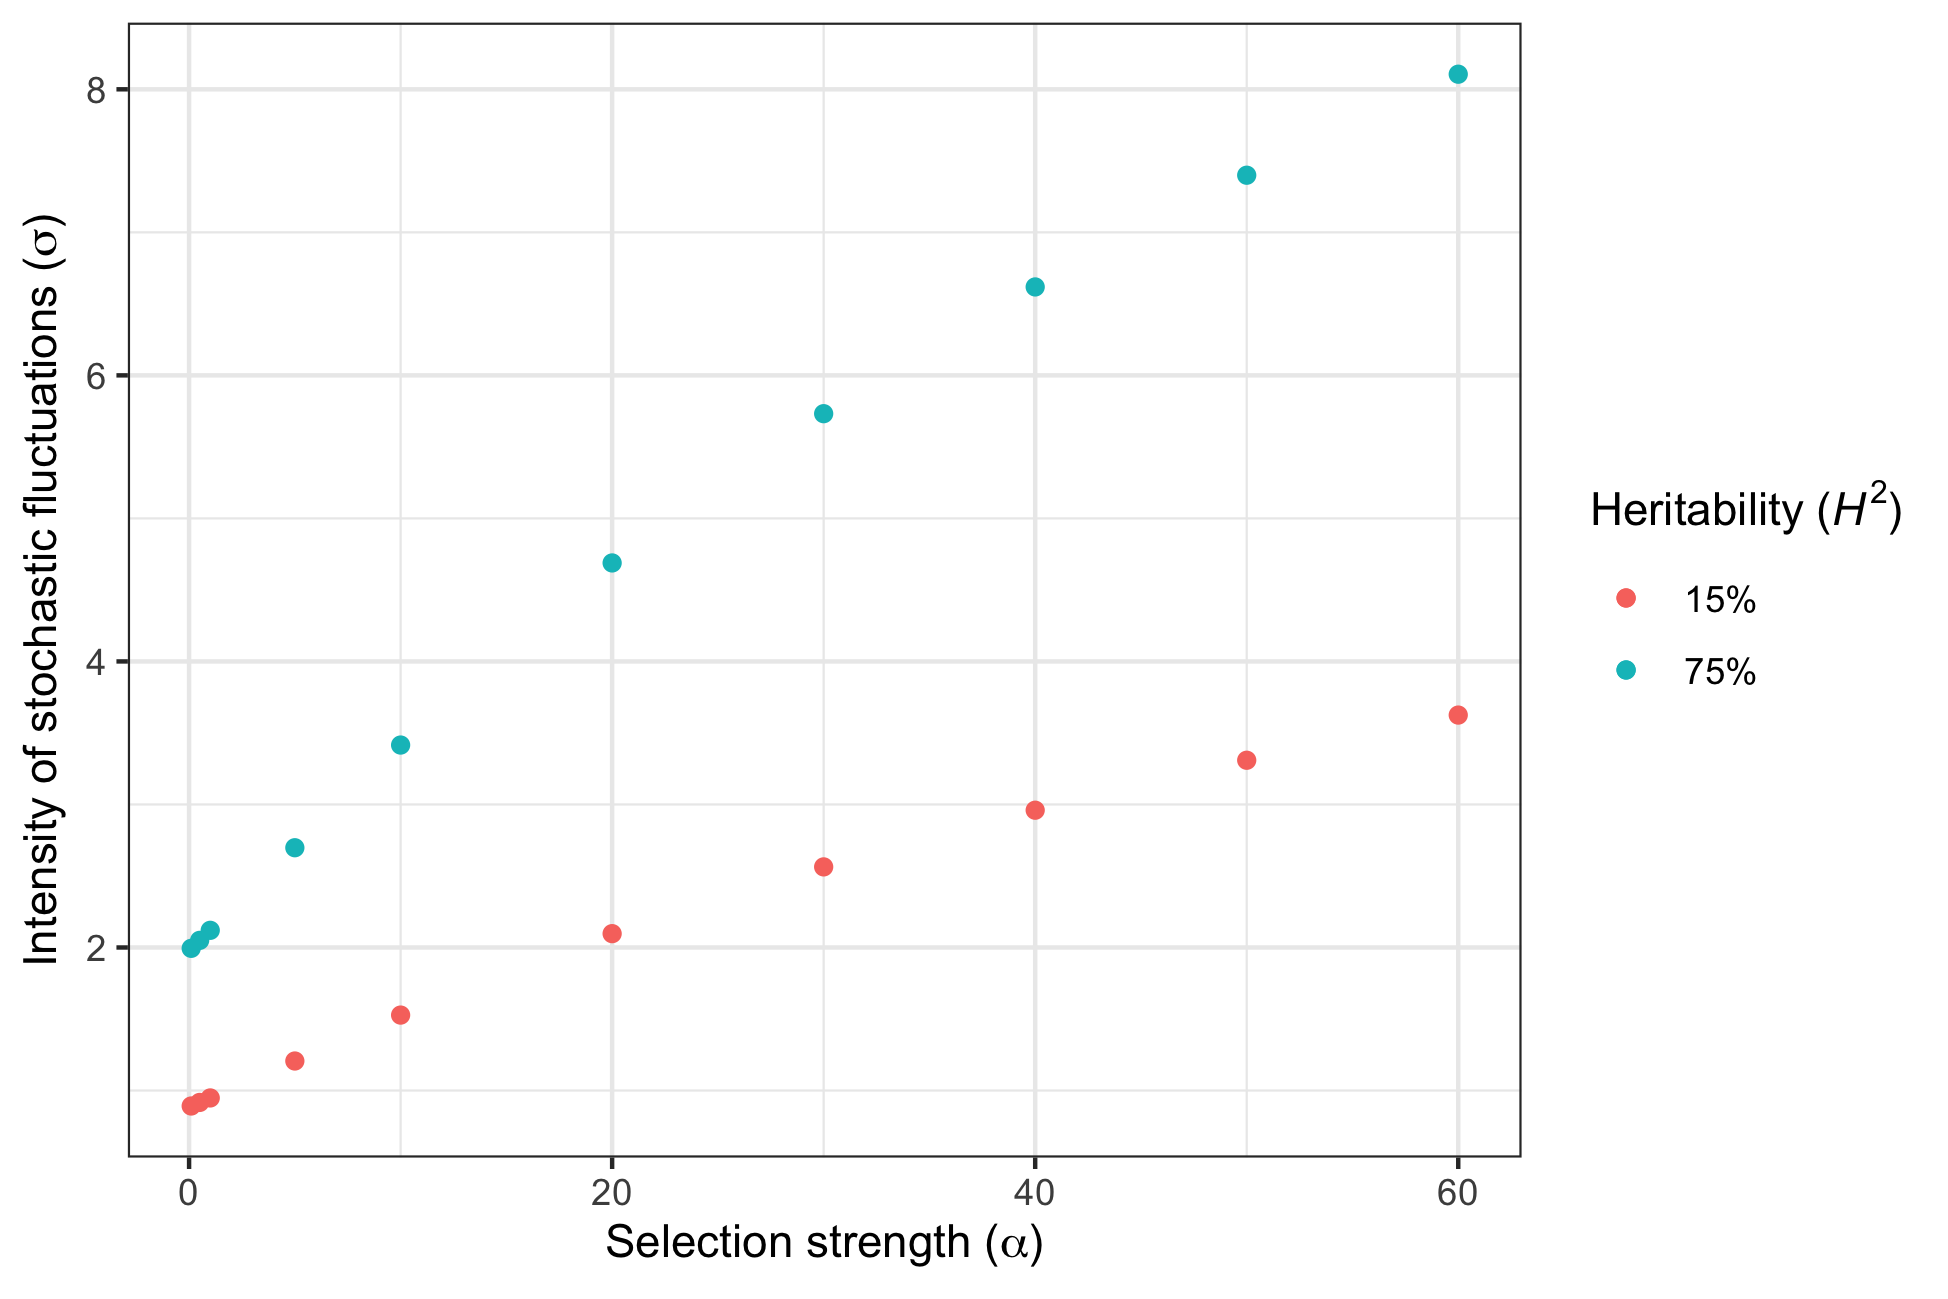
\includegraphics[width = 0.7\linewidth]{figures/sigma_vs_alpha.png}
	\DIFaddendFL \caption{\DIFaddbeginFL \DIFaddFL{Relationship between the selection strength parameter $\alpha$ and the intensity of stochastic evolutionary fluctuations parameter $\sigma$ at two different heritability ($H^2$) values in the  simulation scheme. $\sigma$ was determined as a function of $\alpha$ and $H^2$ under the POUMM (function given in Table \ref{tab:sim-params}).}}
	\label{fig:sigma-vs-alpha}
	\end{center}
\end{figure}

\begin{figure}[H]
	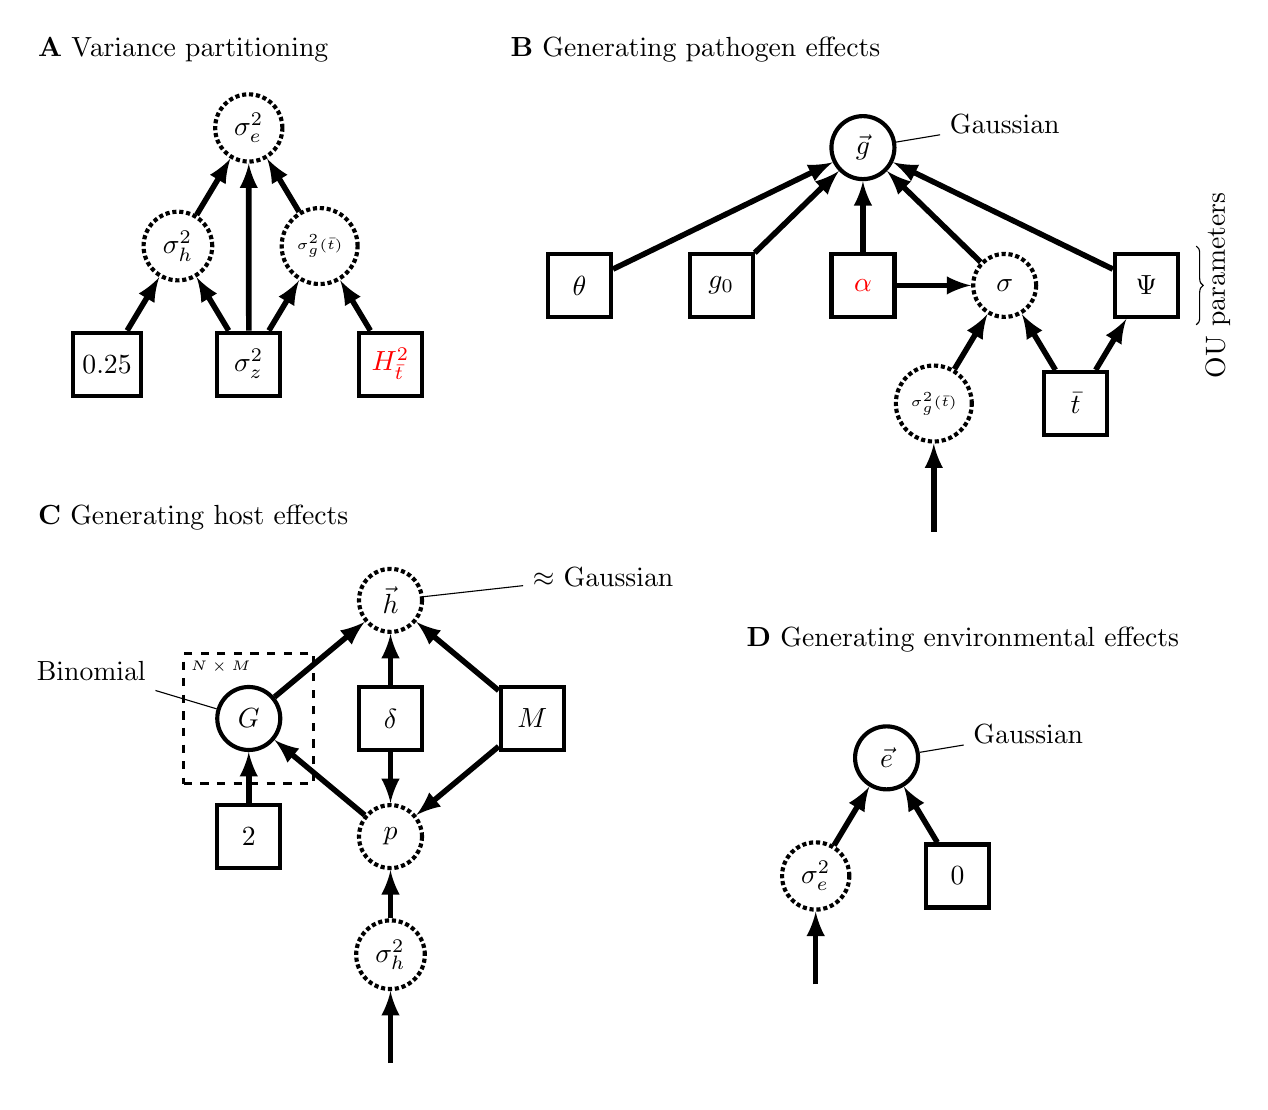
\begin{tikzpicture}

	% Variance 
	\begin{scope}[xshift = 0cm, yshift = 0cm]
	\node[anchor = west] (alabel) at (-1, 4) {\textbf{A} Variance partitioning};
	\node[constnode] (H2h) at (0, 0) {0.25};
	\node[constnode] (varz) at ($(H2h) + (1.8, 0)$) {$\sigma^2_z$};
	\node[constnode] (H2) at ($(H2h) + (3.6, 0)$) {\textcolor{red}{$H^2_{\bar{t}}$}};
	\node[detnode] (varh) at ($(H2h) + (0.9, 1.5)$) {$\sigma^2_{h}$};
	\node[detnode] (varv) at ($(varz) + (0.9, 1.5)$) {\tiny $\sigma^2_{g}(\bar{t})$};
	\node[detnode] (vare) at ($(varh) + (0.9, 1.5)$) {$\sigma^2_{e}$};
	\draw[taro] (H2h) -- (varh);
	\draw[taro] (varz) -- (varh);
	\draw[taro] (varz) -- (varv);
	\draw[taro] (H2) -- (varv);
	\draw[taro] (varh) -- (vare);
	\draw[taro] (varv) -- (vare);
	\draw[taro] (varz) -- (vare);
	\end{scope}

	% Virus
	\begin{scope}[xshift = 6cm, yshift = -0.5cm]
	\node[anchor = west] (blabel) at (-1, 4.5) {\textbf{B} Generating pathogen effects};
	\node[constnode] (theta) at (0, 1.5) {$\theta$};
	\node[constnode] (g0) at (1.8, 1.5) {$g_{0}$};
	\node[constnode] (alpha) at (3.6, 1.5) {\textcolor{red}{$\alpha$}};
	\node[detnode] (sigma) at (5.4, 1.5) {$\sigma$};
	\node[constnode] (tree) at (7.2, 1.5) {$\Psi$};
	\node[detnode] (varv) at (3.6+0.9, 0) {\tiny $\sigma^2_{g}(\bar{t})$};
	\node[constnode] (tbar) at (3.6+0.9+1.8, 0) {$\bar{t}$};
	\node[snode] (v) at (3.6, 3.25) {$\vec{g}$};
	\draw[taro] (theta) -- (v);
	\draw[taro] (g0) -- (v);
	\draw[taro] (alpha) -- (v);
	\draw[taro] (sigma) -- (v);
	\draw[taro] (tree) -- (v);
	\draw[taro] (varv) -- (sigma);
	\draw[taro] (tbar) -- (sigma);
	\draw[taro] (tbar) -- (tree);
	\draw[taro] (alpha) -- (sigma);
	\node[white] (varpic) at (3.6+0.9, -1.75) {};
	\draw[taro] (varpic) -- (varv);
	\node (vdist) at ($(v) + (1.8, 0.3)$) {Gaussian};
	\draw (v) -- (vdist);
	\draw[decoration={brace, mirror, raise=18pt}, sloped, decorate] (7.2, 1.5 - .5) -- node[below = 18pt] {OU parameters} (7.2, 1.5 + .5);
	\end{scope}

	% Host 
	\begin{scope}[xshift = 0cm, yshift = -7.5cm]
	\node[anchor = west] (clabel) at (-1, 5.55) {\textbf{C} Generating host effects};
	\node[constnode] (d) at (1.8, 1.5) {2};
	\node[detnode] (p) at (3.6, 1.5) {$p$};
	\node[snode] (G) at (1.8, 3) {$G$};
	\node[rectangle, dashed, very thick, inner sep=4mm, draw=black!100, fit = (G) ] (Gplate) {};
	\node[anchor=north west, inner sep=3pt] at (Gplate.north west) {\tiny $N\times M$};
	\node[detnode] (varh) at (3.6, 0) {$\sigma^2_{h}$};
	\node[constnode] (delta) at (3.6, 3) {$\delta$};
	\node[detnode] (h) at (3.6, 4.5) {$\vec{h}$};
	\node[constnode] (M) at (5.4, 3) {$M$};
	\draw[taro] (d) -- (G);
	\draw[taro] (p) -- (G);
	\draw[taro] (varh) -- (p);
	\draw[taro] (delta) -- (p);
	\draw[taro] (M) -- (p);
	\draw[taro] (M) -- (h);
	\draw[taro] (delta) -- (h);
	\draw[taro] (G) -- (h);
	\node[white] (varpic) at (3.6, -1.5) {};
	\draw[taro] (varpic) -- (varh);
	\node (hdist) at ($(h) + (2.7, 0.3)$) {$\approx$ Gaussian};
	\draw (h) -- (hdist);
	\node (gdist) at ($(G) + (-2, 0.6)$) {Binomial};
	\draw (G) -- (gdist);
	\end{scope}

	% Environment
	\begin{scope}[xshift = 9cm, yshift = -6.5cm]
	\node[anchor = west] (dlabel) at (-1, 3) {\textbf{D} Generating environmental effects};
	\node[detnode] (vare) at (0, 0) {$\sigma^2_{e}$};
	\node[constnode] (zero) at ($(vare) + (1.8, 0)$) {0};
	\node[snode] (e) at ($(vare) + (1.8/2, 1.5)$) {$\vec{e}$};
	\draw[taro] (zero) -- (e);
	\draw[taro] (vare) -- (e);
	\node[white] (varpic) at (0, -1.5) {};
	\draw[taro] (varpic) -- (vare);
	\node (edist) at ($(e) + (1.8, 0.3)$) {Gaussian};
	\draw (e) -- (edist);
	\end{scope}

	\end{tikzpicture}
	\caption{\DIFaddendFL A graphical model representation of our simulation scheme, following the recommendations in \cite{Hohna2014}. Variables in solid squares are constants, with the two master control variables that we vary from simulation to simulation highlighted in red. Variables in solid circles are realizations of random variables and variables in dashed circles are determined as a function of other variables. Arrows represent dependencies among variables and the dashed square represents repetition. All parameters are defined in Table \ref{tab:sim-params}, as well as the values or expressions used for them. (A) shows how the variance in the simulated environmental effect \DIFdelbeginFL \DIFdelFL{$\sigma^2_{\epsilon}$ }\DIFdelendFL \DIFaddbeginFL \DIFaddFL{$\sigma^2_{e}$ }\DIFaddendFL is smaller if the master pathogen heritability value $H^2_{\bar{t}}$ is higher and vice-versa. (B) shows the OU parameters and the pathogen phylogeny, which generate the Gaussian-distributed pathogen effects. The OU parameters $\theta$ and $g_0$ are fixed, whereas $\sigma$ is a deterministic function of the variance in the pathogen effect and the value of $\alpha$. In other words, we use $\sigma$ to maintain the desired pathogen heritability while varying $\alpha$. \DIFdelbeginFL \DIFdelFL{We generate a new random phylogeny for each simulation. }\DIFdelendFL (C) shows how host genotypes are drawn to generate host effects. The host genotype matrix $G$ contains the number of copies (0, 1, or 2) for each of $M$ causal variants with effect size $\delta$. We assume half the variants have a positive effect and half have a negative effect. The allele frequency $p$ for the causal variants set so that we achieve the desired variance in the host effects. (D) shows that the environmental effect is drawn from a Gaussian distribution with mean zero and variance as determined in part (A).}
	\label{fig:sim-design}
\end{figure}

\begin{figure}[H]
\DIFaddbeginFL \begin{center}
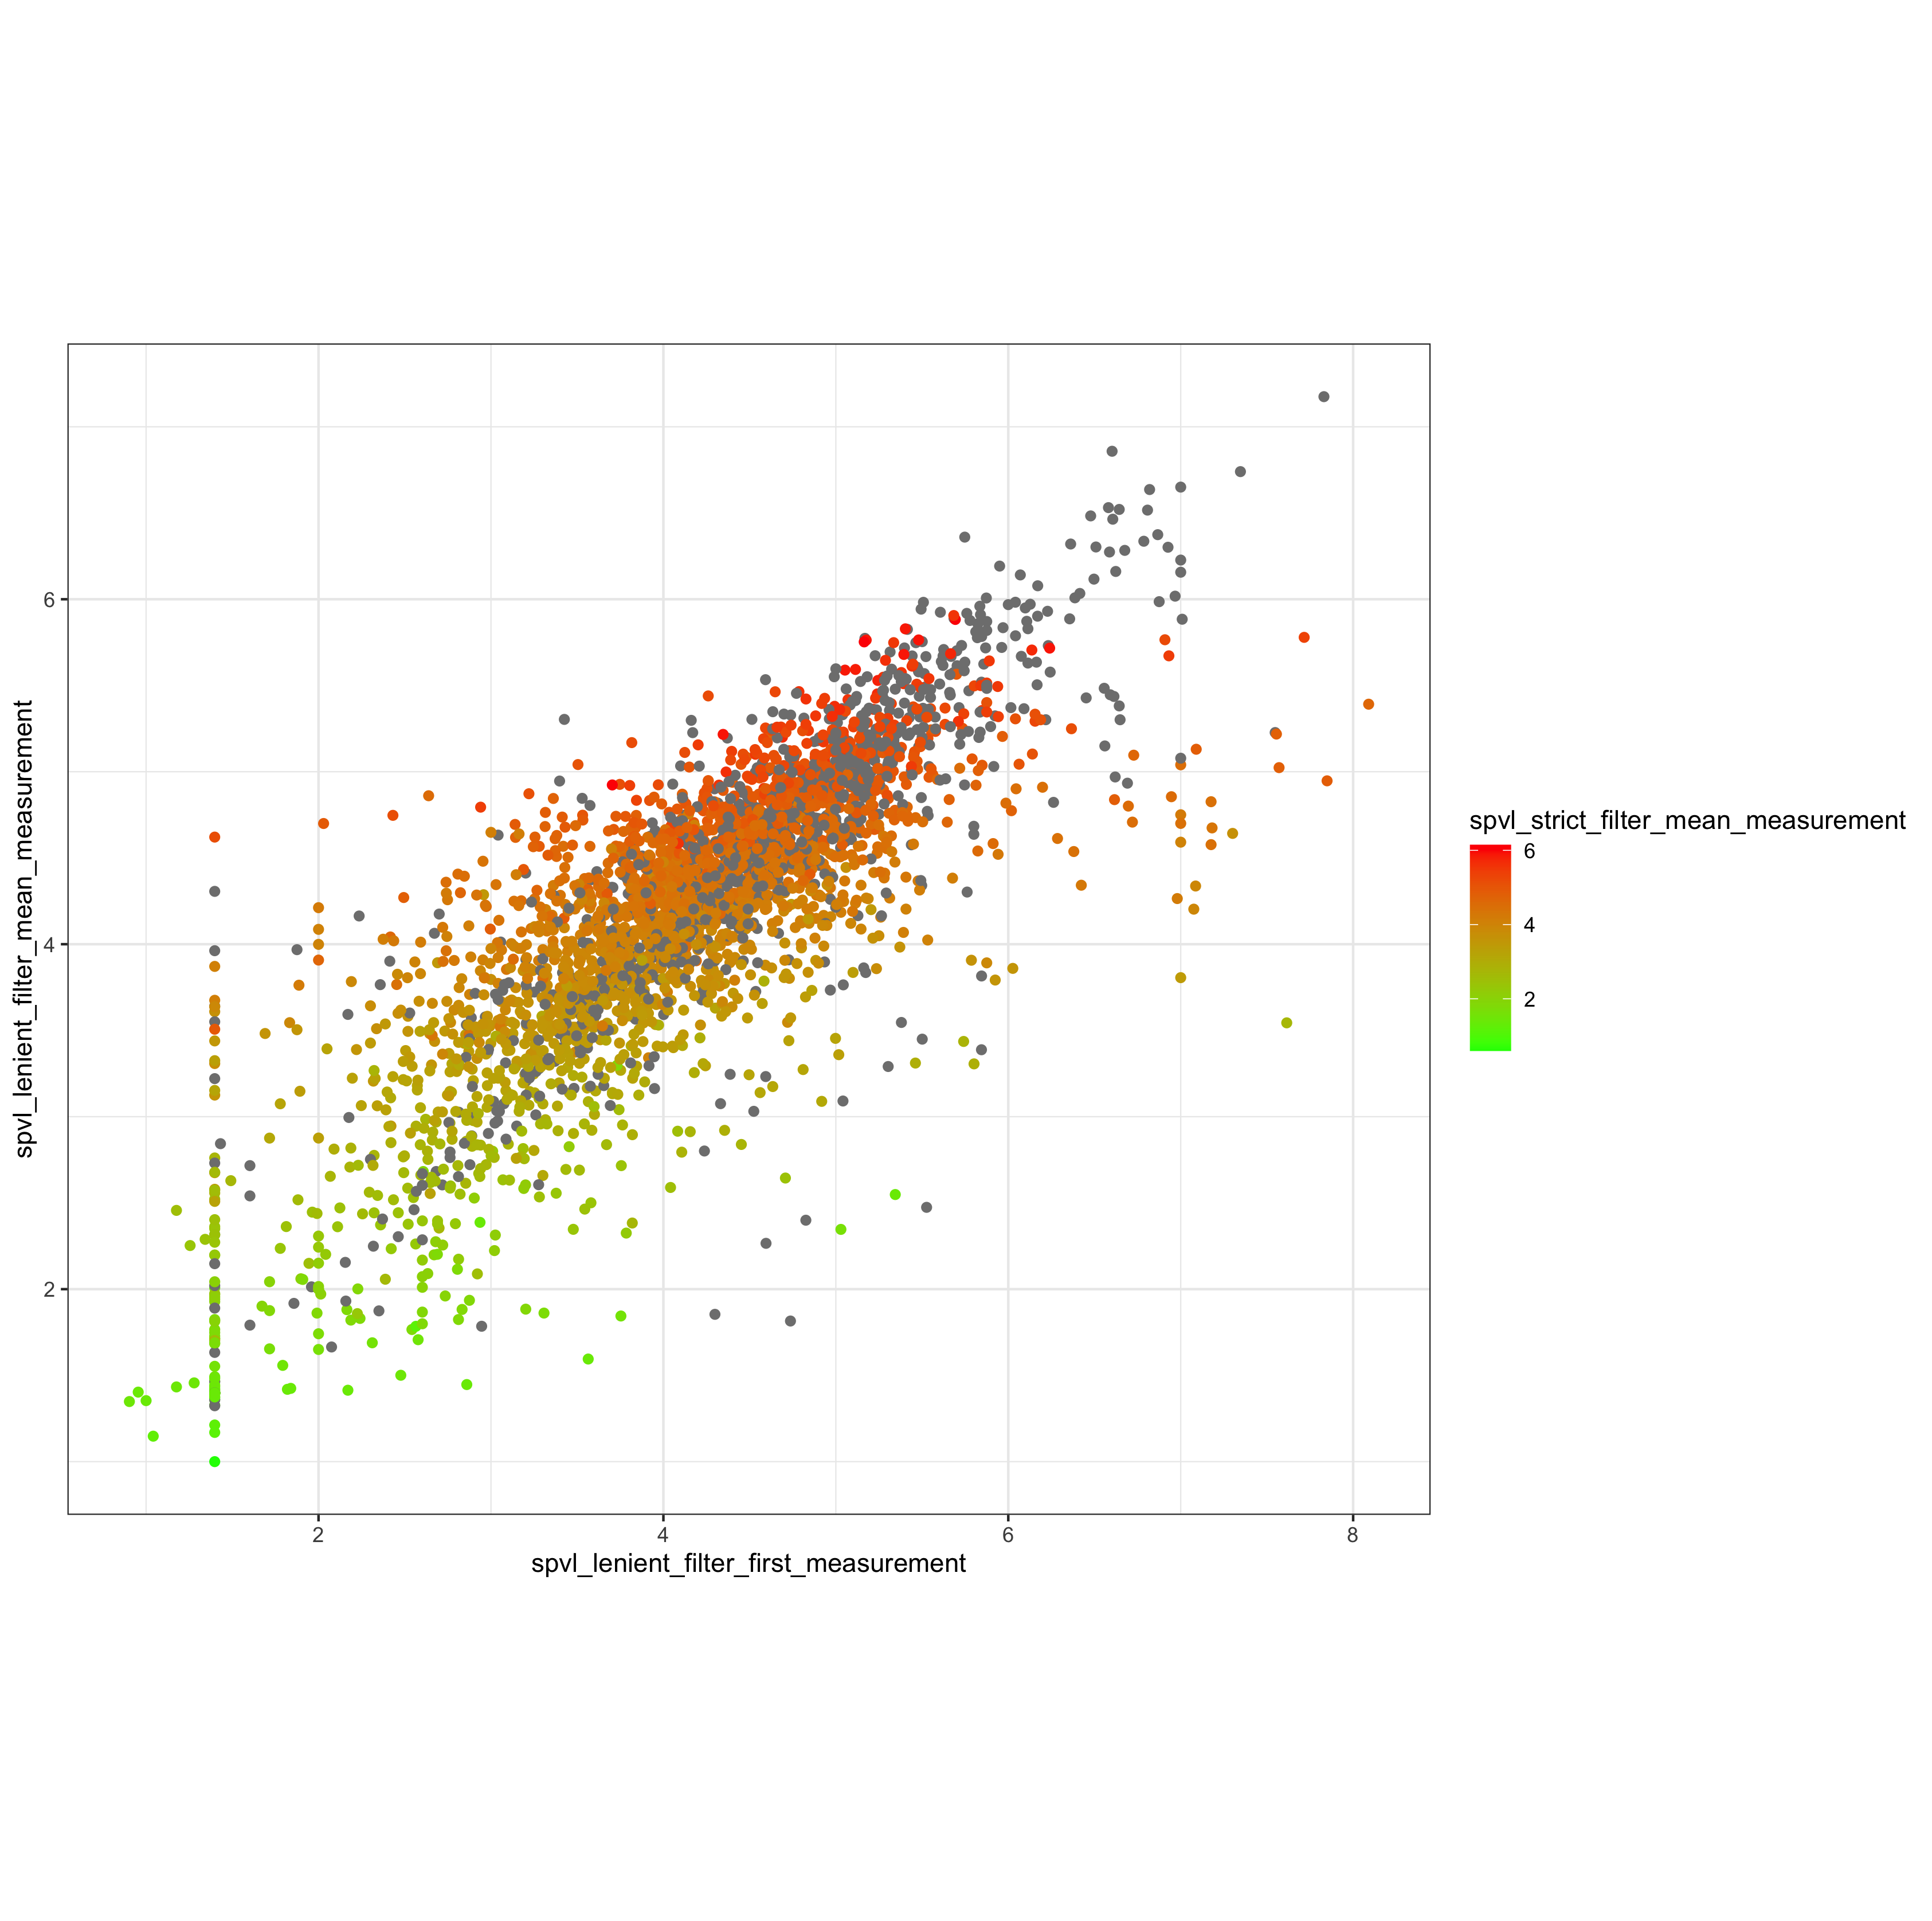
\includegraphics[width = 0.7\linewidth]{figures/spvl_calculation_comparison.png}
	\caption{\DIFaddFL{A comparison of different ways to calculate spVL based on viral load measurements provided by the SHCS. The stricter filtering excludes all measurements possibly $<$ 6 months after infection and after treatment or AIDS, whereas the more lenient filtering excludes only measurements after treatment. We used the lenient filter, mean measurement values because these correlate well with the values from the stricter filter but allow us to retain many more individuals from the cohort for our study.}}
	\label{fig:spvl-calc-comparison}
	\end{center}
\end{figure}

\begin{figure}[H]
	\DIFaddendFL \centering
		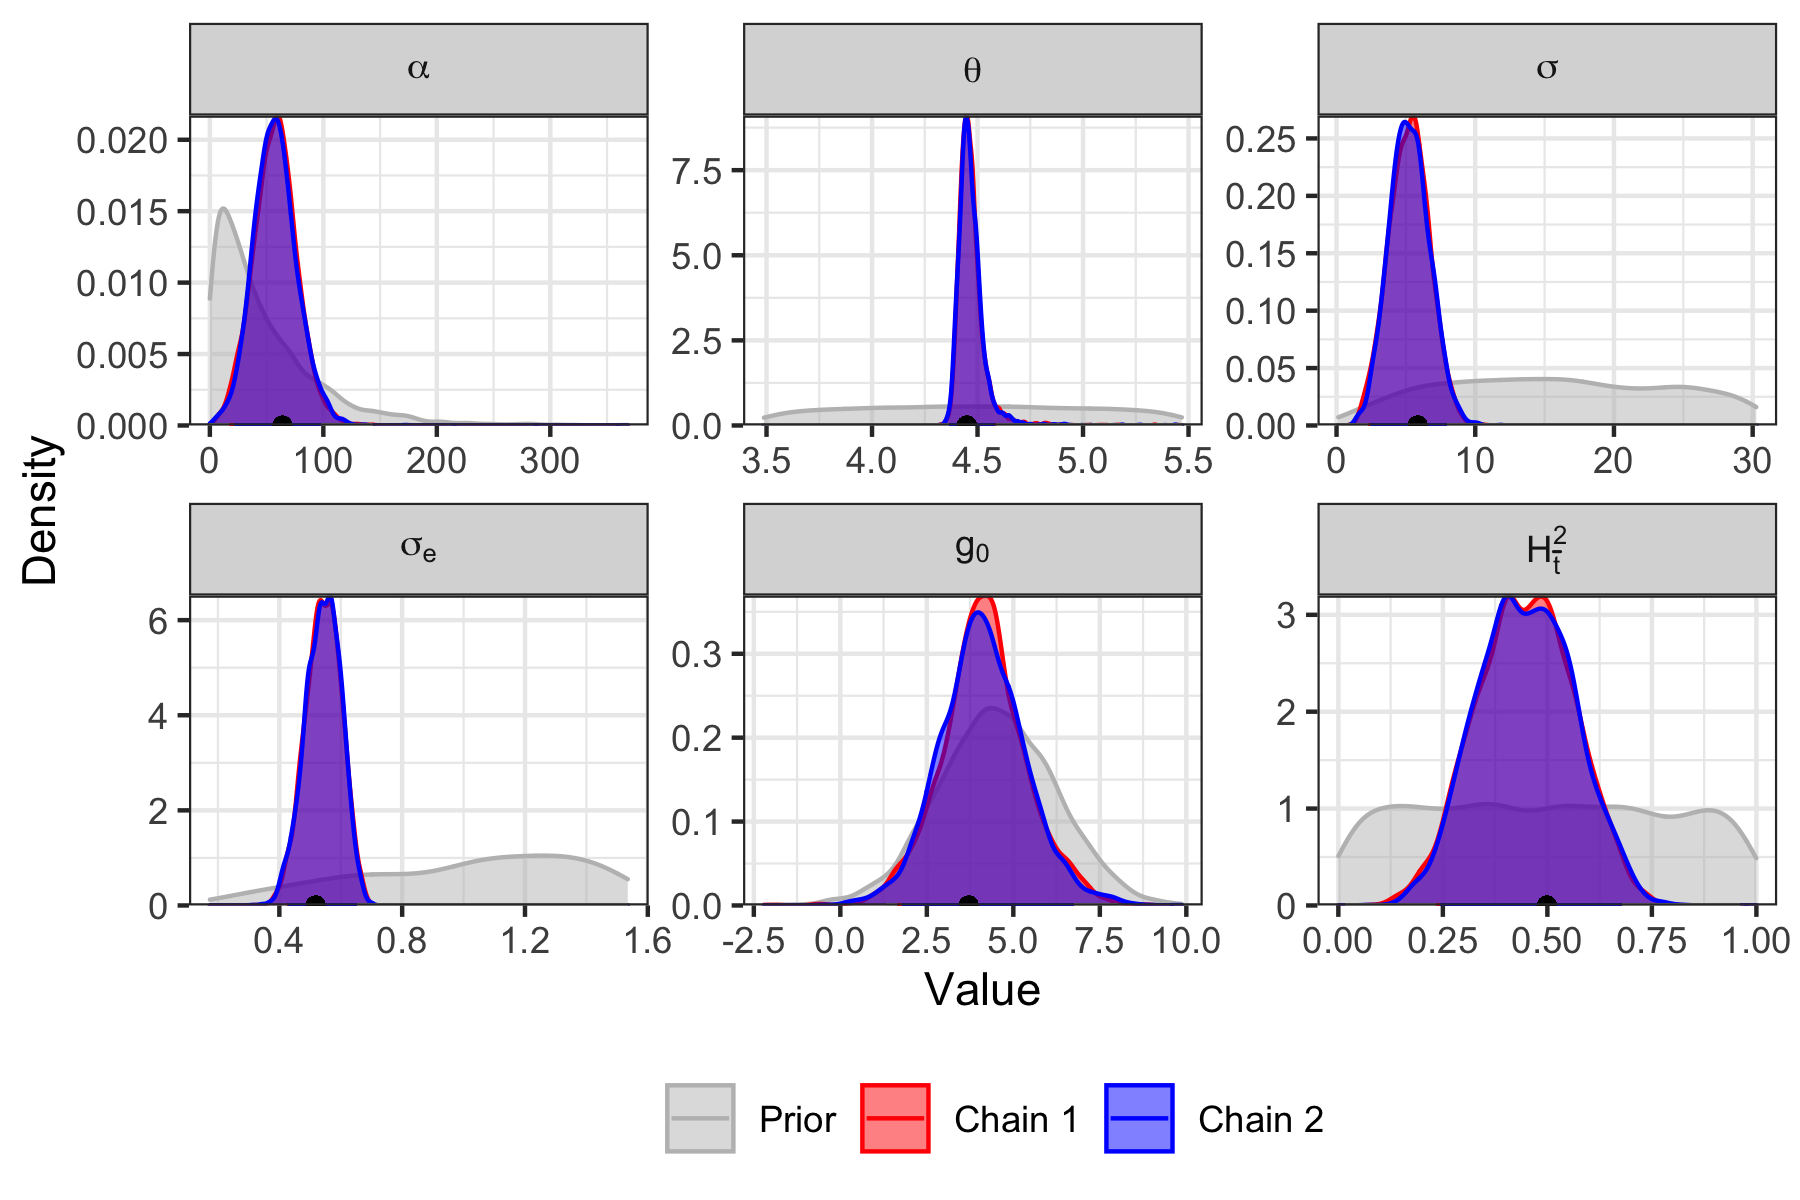
\includegraphics[width=0.7\linewidth]{figures/poumm_parameter_estimates.png}
		\caption{Posterior distributions compared to the prior for POUMM parameter estimates based on \DIFdelbeginFL \DIFdelFL{Swiss }\DIFdelendFL \DIFaddbeginFL \DIFaddFL{HIV-1 spVL }\DIFaddendFL data \DIFaddbeginFL \DIFaddFL{from the SHCS}\DIFaddendFL . We ran two different MCMC chains to ensure the estimates converged.\DIFdelbeginFL \DIFdelFL{The black point on the x-axis shows the posterior mean value, which was used to estimate the pathogen- and non-pathogen effects on spVL.}\DIFdelendFL }
\label{fig:poumm-parameters}
\end{figure}

\begin{figure}[H]
\begin{center}
\DIFdelbeginFL %DIFDELCMD < 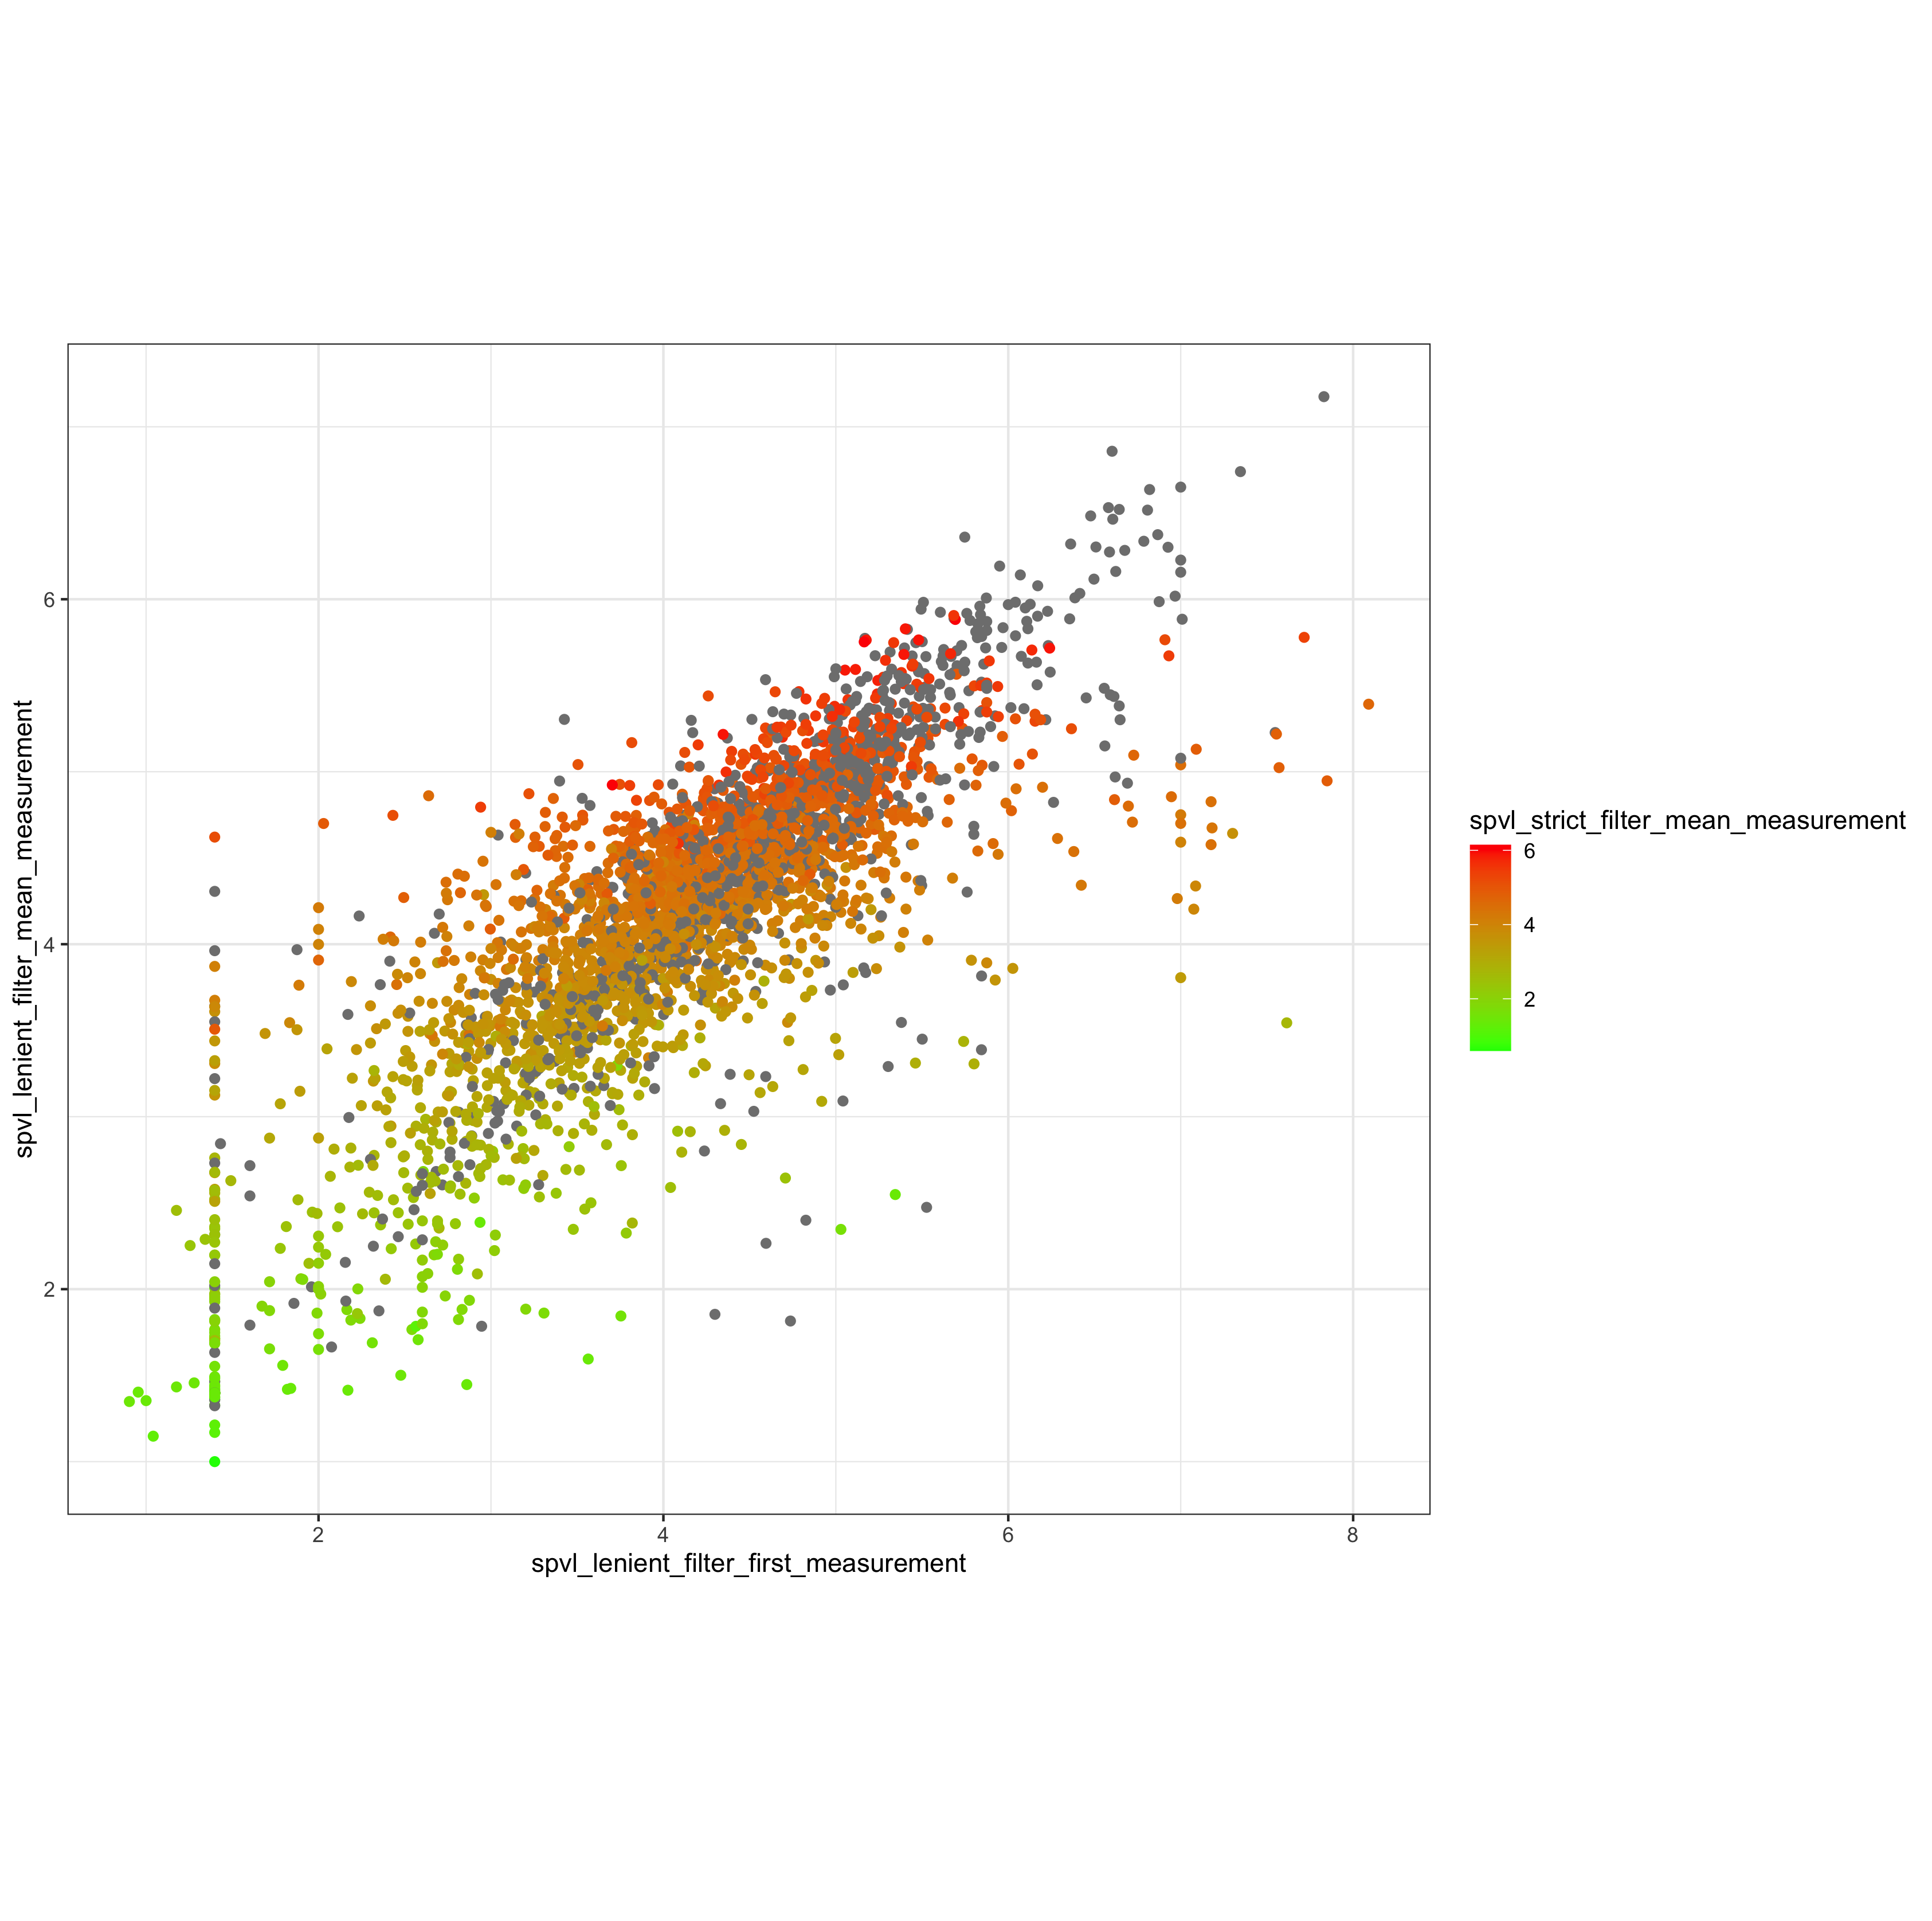
\includegraphics[width = 0.7\linewidth]{figures/spvl_calculation_comparison.png}
%DIFDELCMD < 	%%%
%DIFDELCMD < \caption{%
{%DIFAUXCMD
\DIFdelFL{A comparison of different ways to calculate spVL based on viral load measurements provided by the SHCS. The stricter filtering excludes all measurements possibly $<$ 6 months after infection and after treatment or AIDS, whereas the more lenient filtering excludes only measurements after treatment. We used the lenient filter, mean measurement values because these correlate well with the values from the stricter filter but allow us to retain many more individuals from the cohort for our study.}}
	%DIFAUXCMD
%DIFDELCMD < \label{fig:spvl-calc-comparison}
%DIFDELCMD < 	%%%
\DIFdelendFL \DIFaddbeginFL 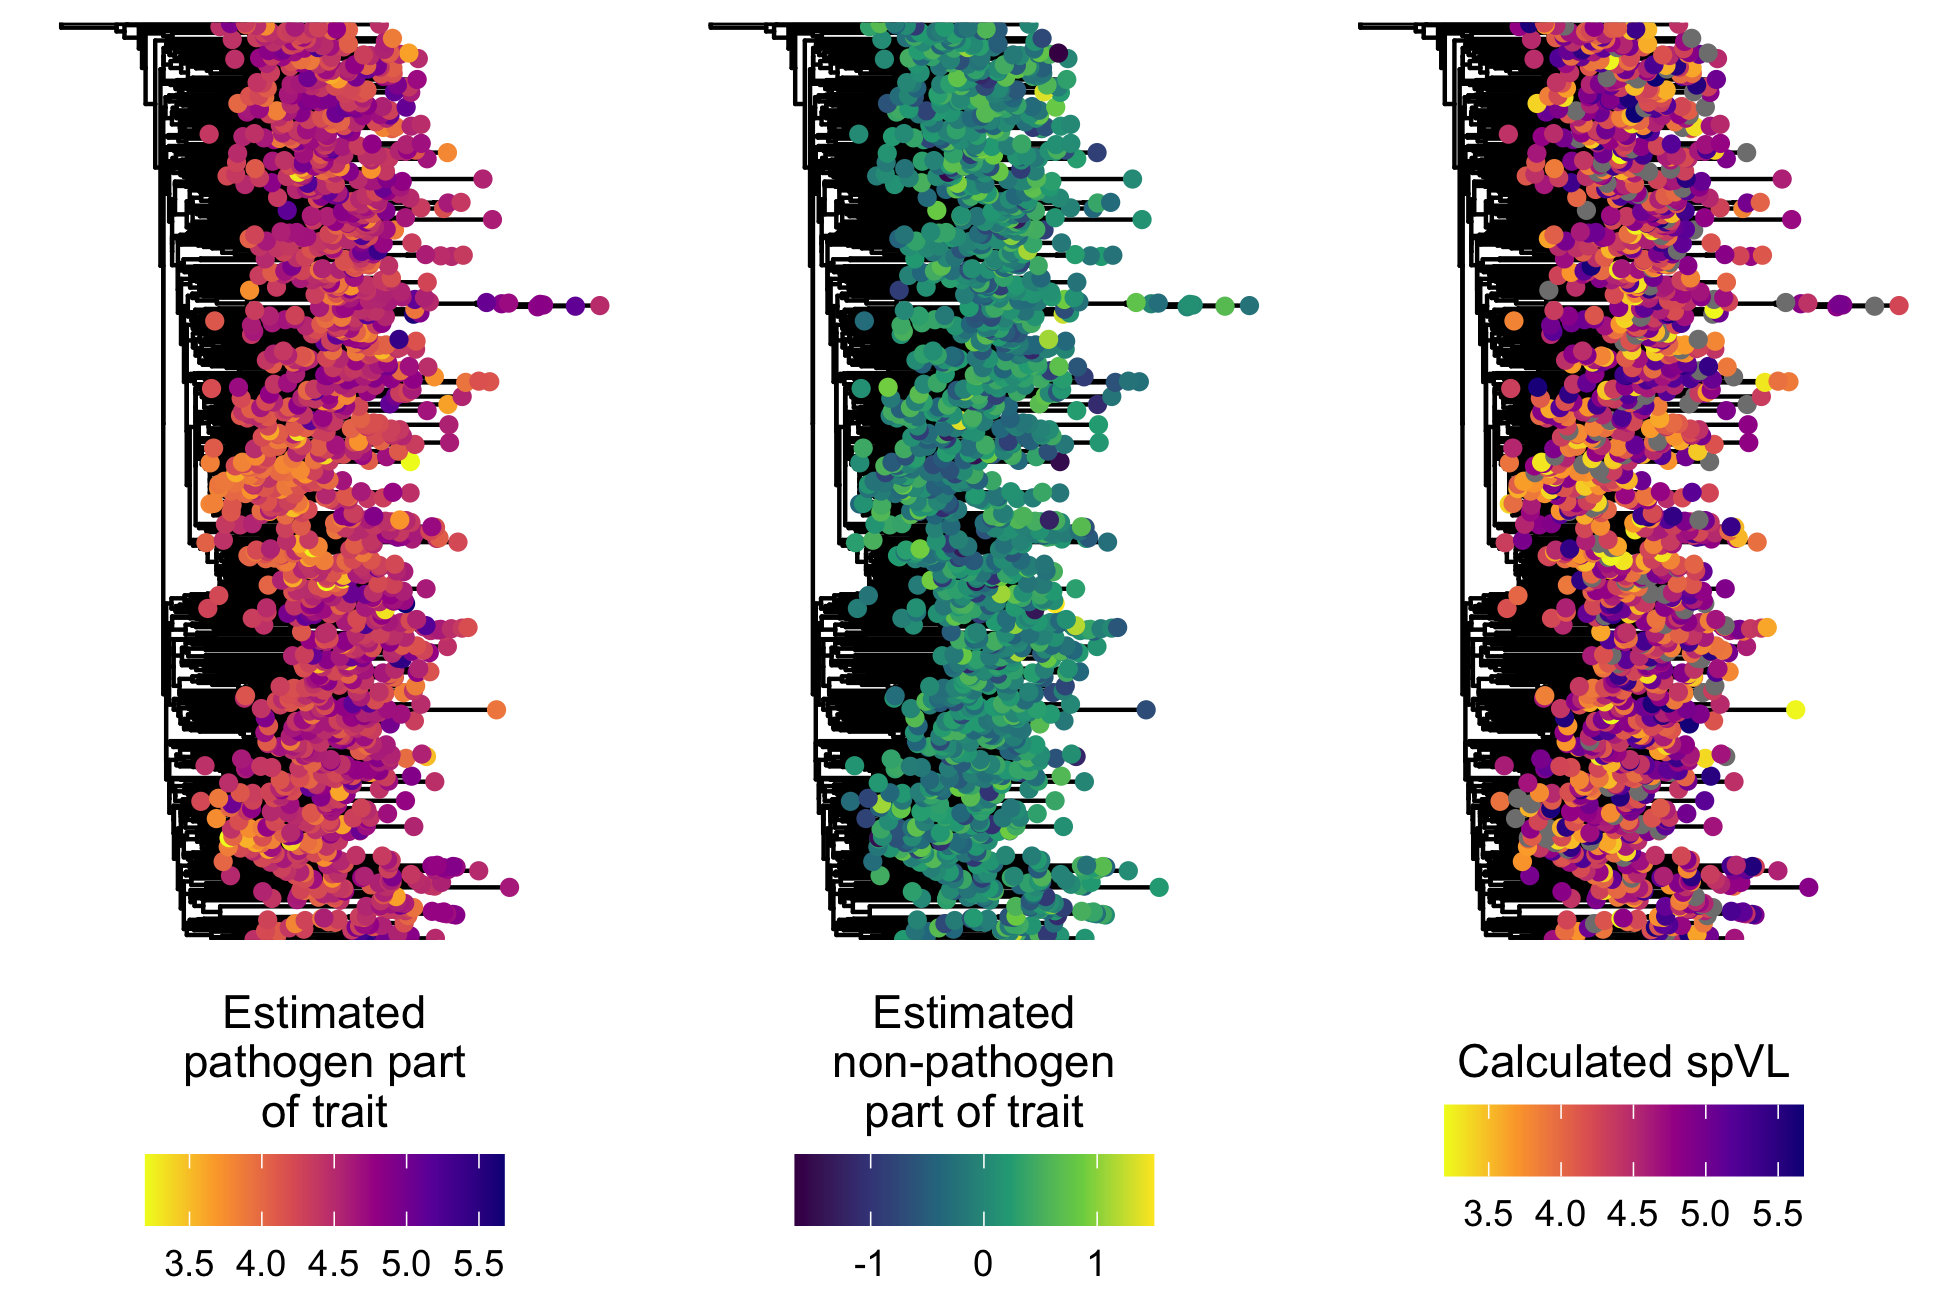
\includegraphics[width = \linewidth]{figures/spvl_on_tree.png}
	\caption{\DIFaddFL{Inferred HIV-1 $pol$ gene phylogeny with tips colored by (A) calculated spVL, (B) estimated non-pathogen effects on spVL and (C) estimated pathogen effects on spVL.}}
	\label{fig:spvl-on-tree}
	\DIFaddendFL \end{center}
\end{figure}

\begin{figure}[H]
\begin{center}
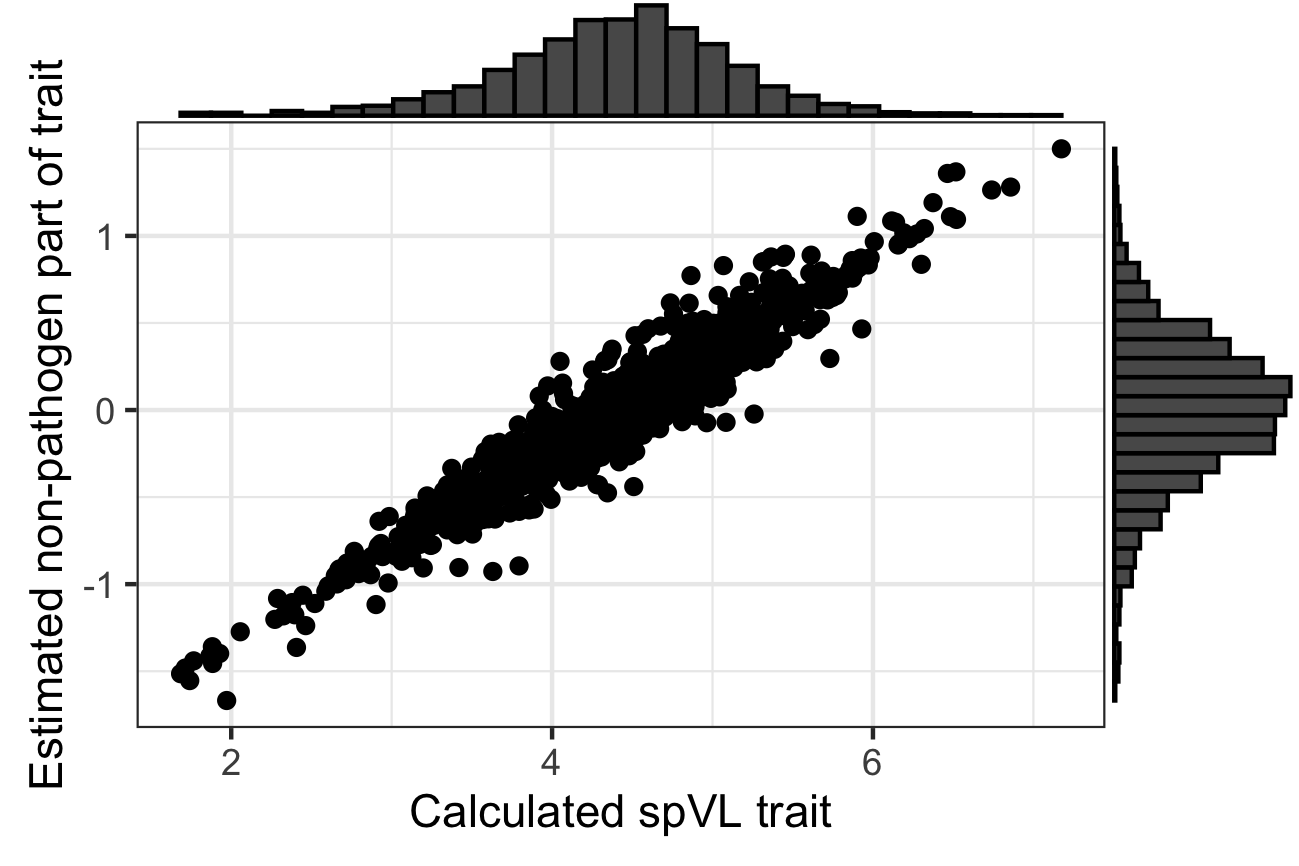
\includegraphics[width = 0.462\linewidth]{figures/trait_values.png}
	\caption{A comparison of measured (calculated) spVL values versus our estimated non-pathogen effect on spVL for each SHCS cohort member used in the study. The histograms show the marginal distribution of each value across the individuals.}
	\label{fig:trait-comparison}
	\end{center}
\end{figure}

\begin{figure}[H]
	\DIFdelbeginFL %DIFDELCMD < \begin{center}
%DIFDELCMD < 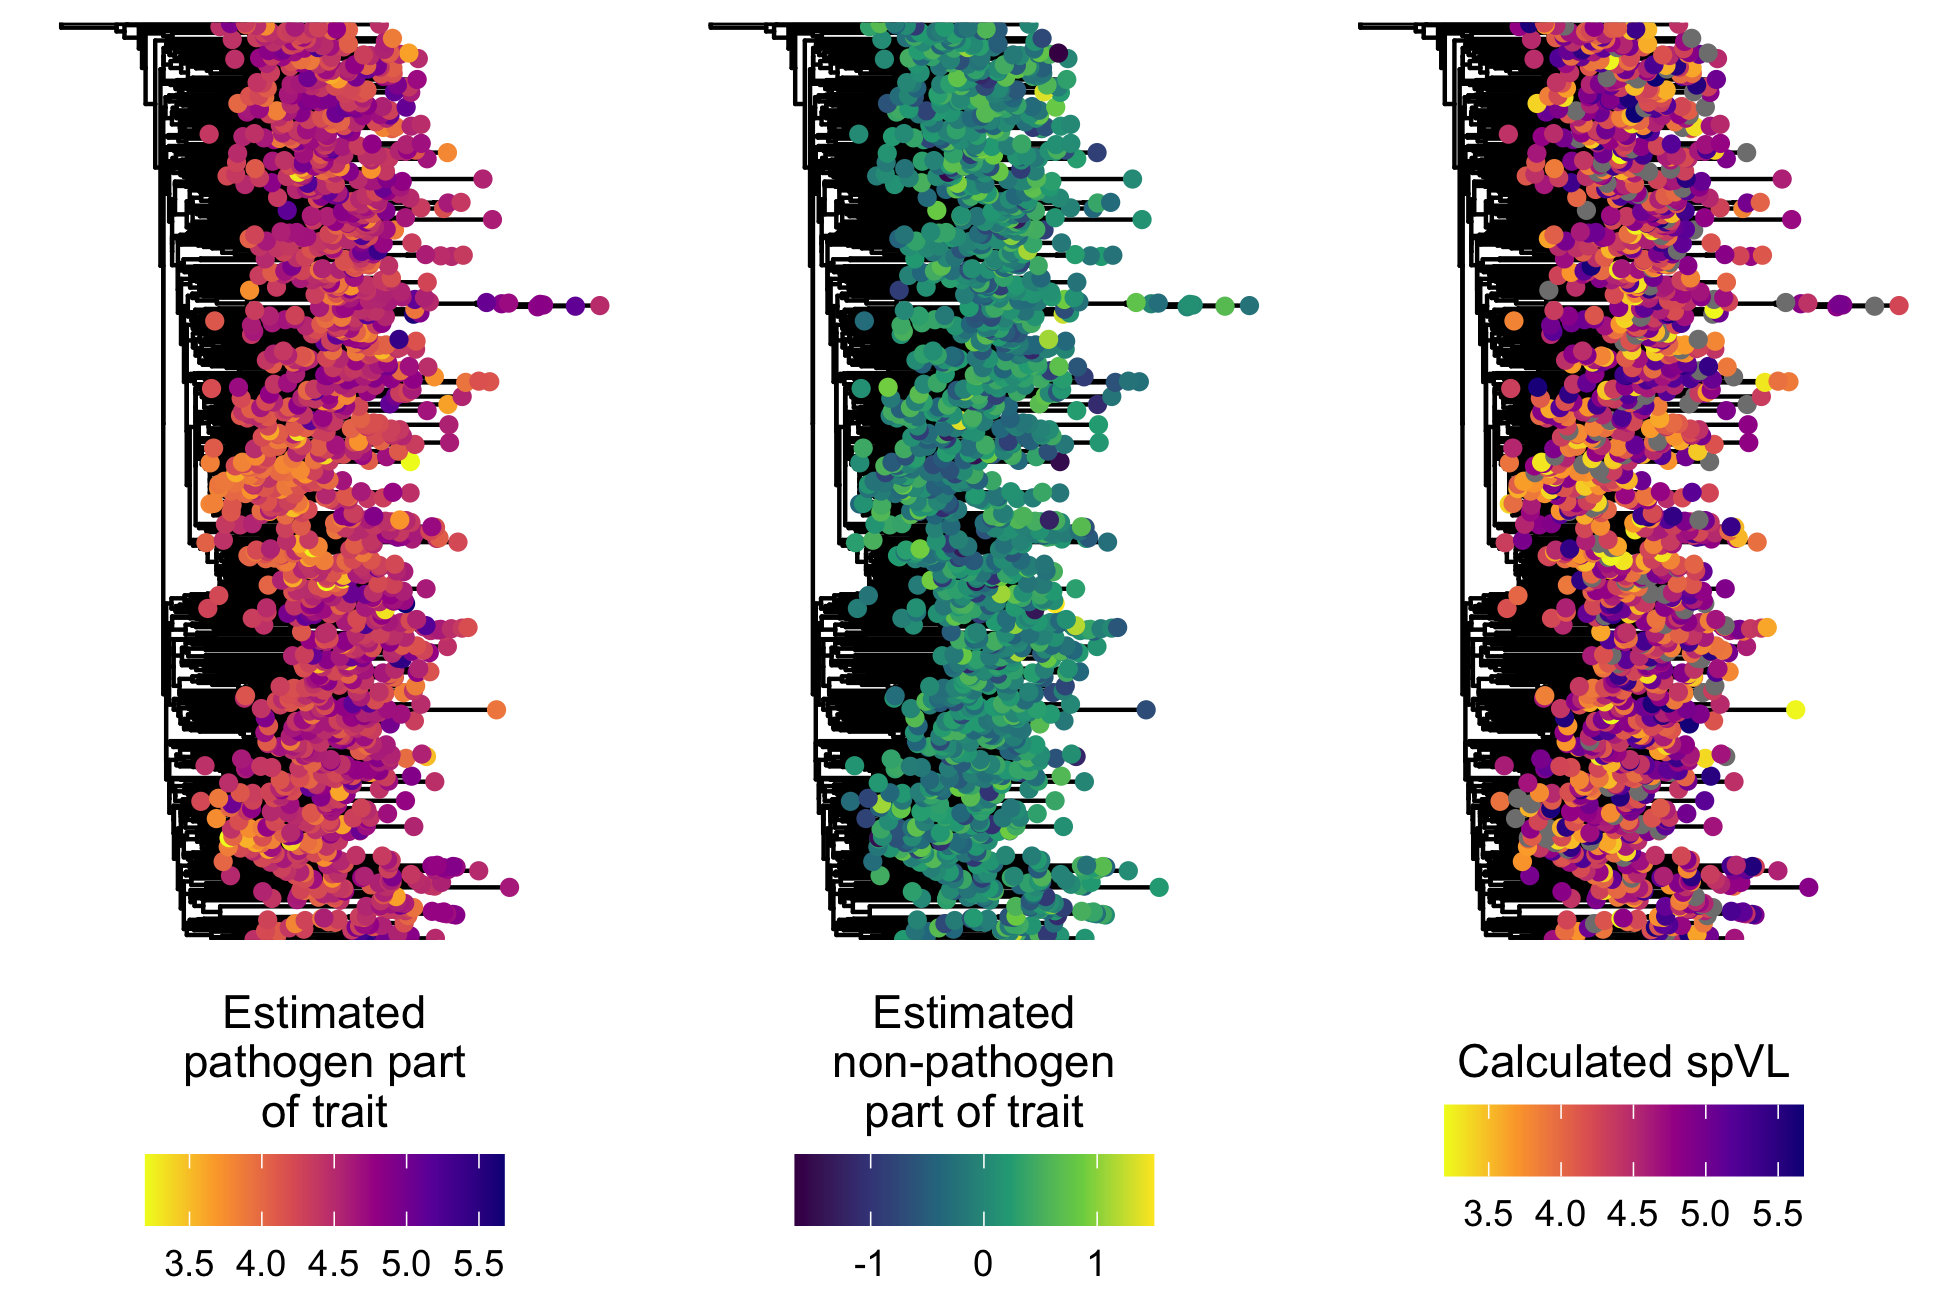
\includegraphics[width = \linewidth]{figures/spvl_on_tree.png}
%DIFDELCMD < 	%%%
%DIFDELCMD < \caption{%
{%DIFAUXCMD
\DIFdelFL{Inferred HIV-1 $pol$ gene phylogeny with tips colored by (A) calculated spVL, (B) estimated non-pathogen effects on spVL and (C) estimated pathogen effects on spVL.}}
	%DIFAUXCMD
%DIFDELCMD < \label{fig:spvl-on-tree}
%DIFDELCMD < 	\end{center}
%DIFDELCMD < \end{figure}
%DIFDELCMD < 

%DIFDELCMD < \begin{figure}[H]
%DIFDELCMD < 	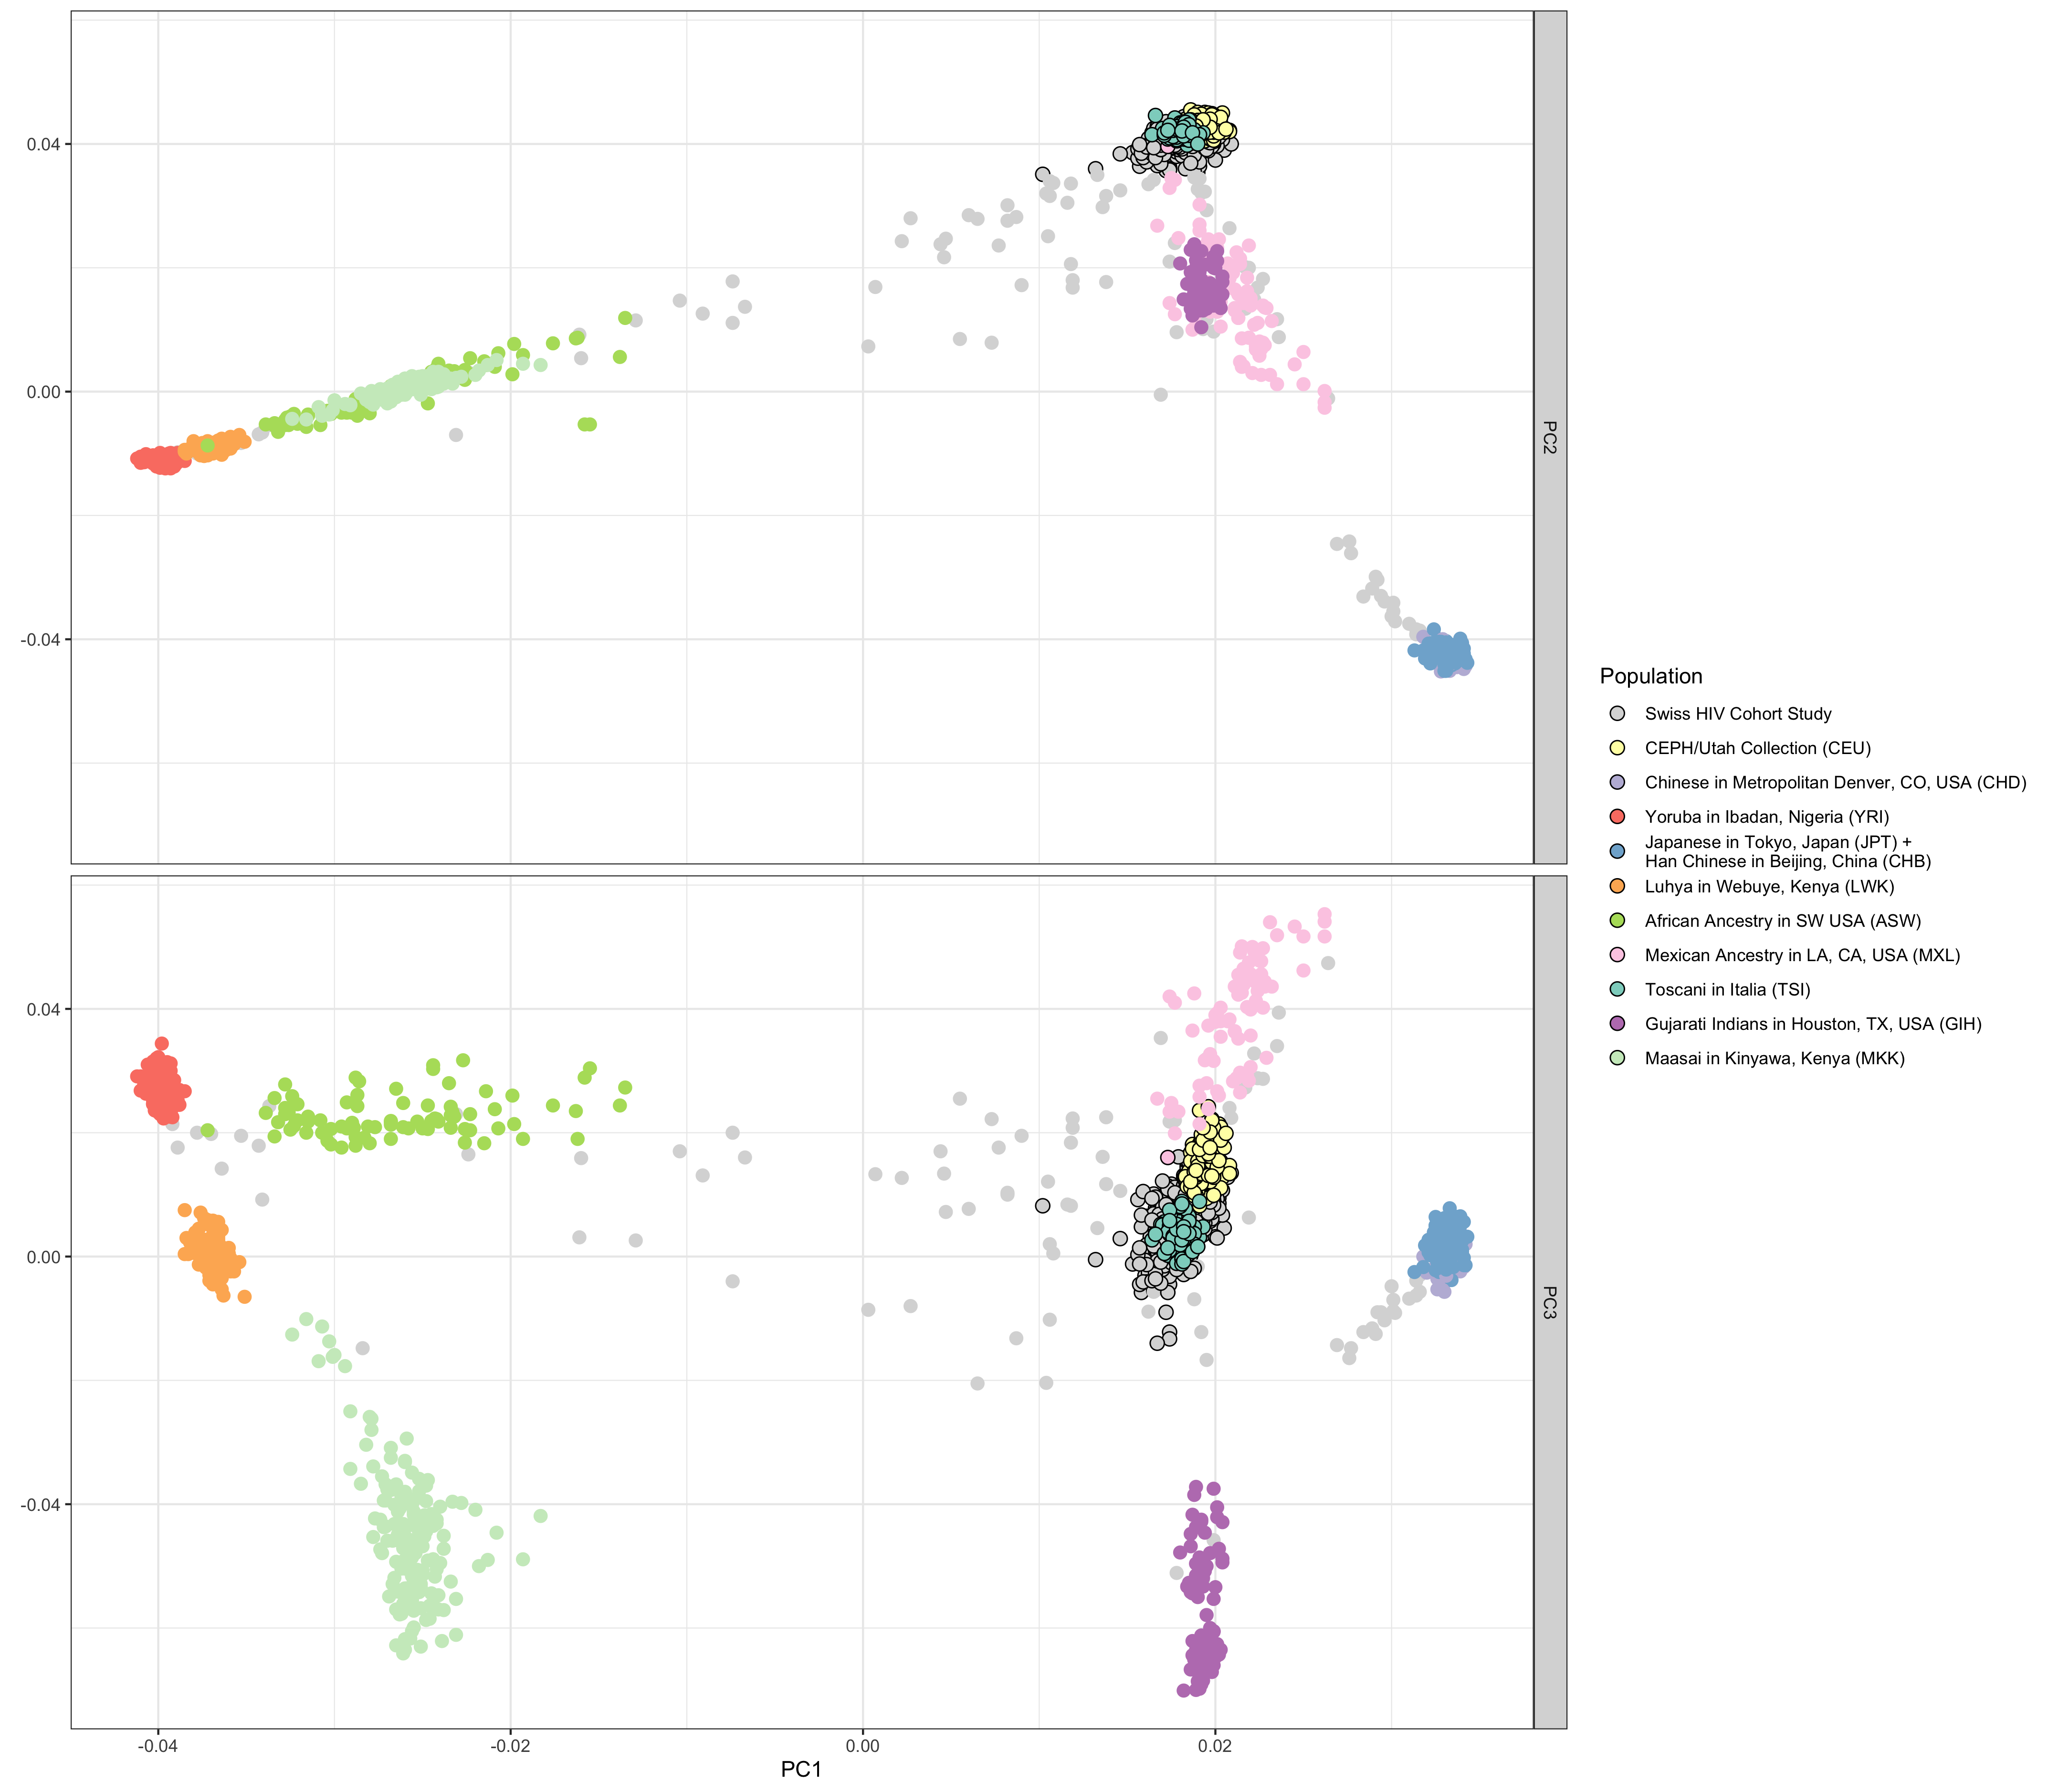
\includegraphics[width=\linewidth]{figures/host_genotype_pca.png}
%DIFDELCMD < 	\caption{%%%
\DIFdelFL{SHCS individuals and HapMap3 individuals plotted along the top three principle components of genetic variation. Points with black borders are within the thresholds used to select individuals of likely European ancestry.}%DIFDELCMD < \MBLOCKRIGHTBRACE
%DIFDELCMD < 	\label{fig:PCA}
%DIFDELCMD < \end{figure}
%DIFDELCMD < 

%DIFDELCMD < \begin{figure}[H]
%DIFDELCMD < 	%%%
\DIFdelendFL \centering
	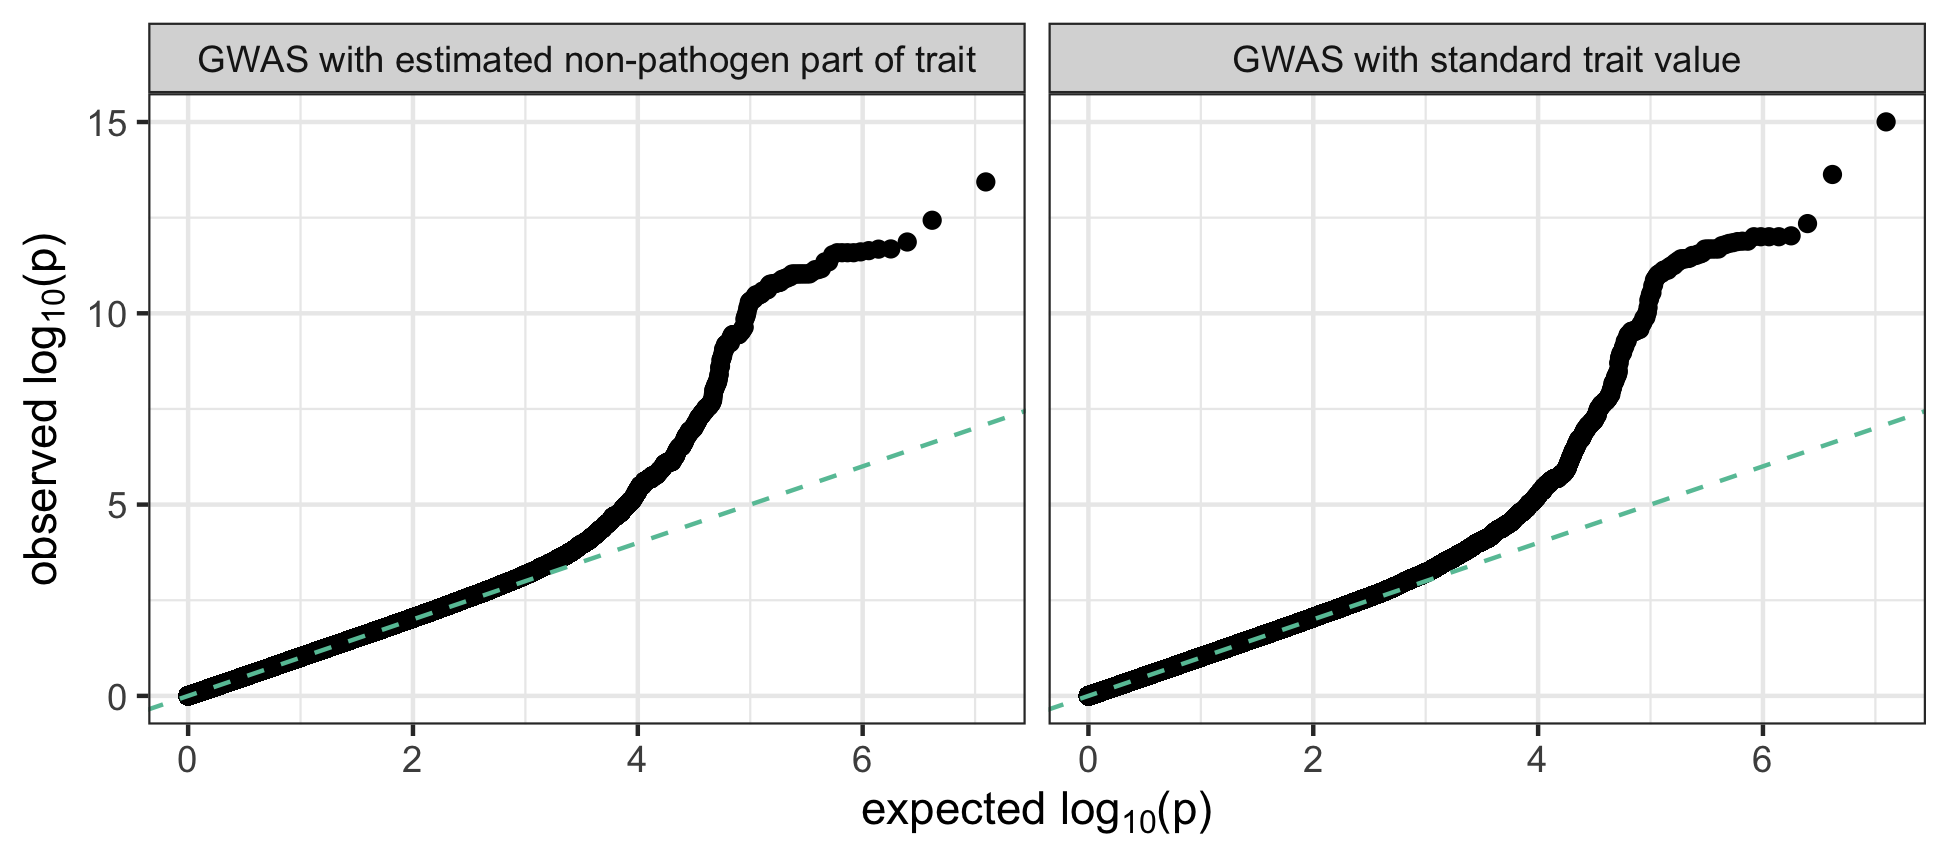
\includegraphics[width=\linewidth]{figures/qq_plots.png}
	\caption{Quartile-quartile plots from \DIFaddbeginFL \DIFaddFL{HIV-1 spVL }\DIFaddendFL association tests. The dashed green line shows the y = x line.}
	\label{fig:qq-plots}
\end{figure}

\DIFaddbegin \begin{figure}[H]
\begin{center}
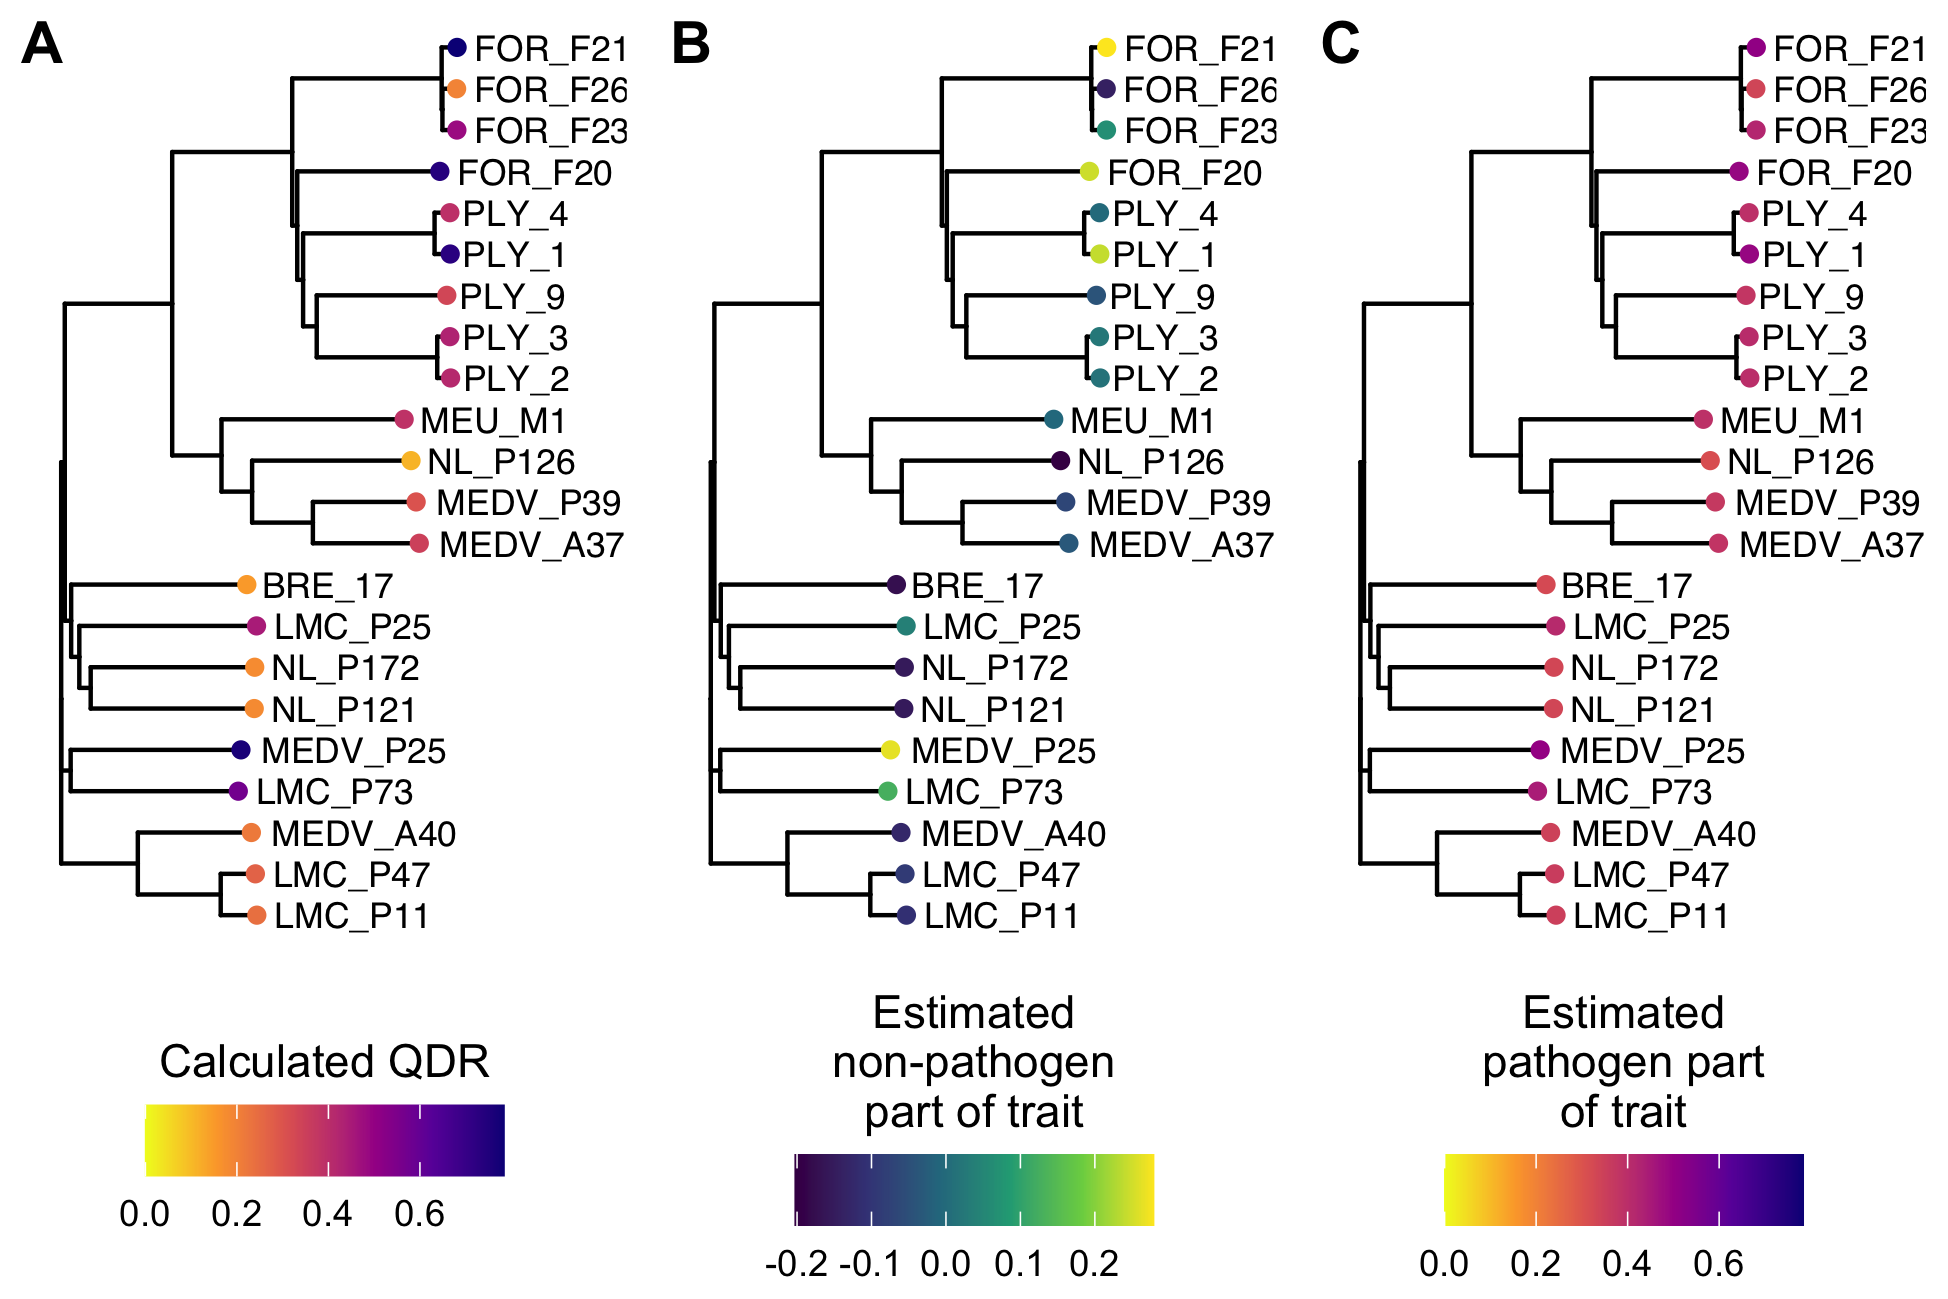
\includegraphics[width = \linewidth]{figures/qdr_on_tree_arboricola.png}
	\caption{\DIFaddFL{Inferred }\emph{\DIFaddFL{X. arboricola}} \DIFaddFL{phylogeny with tips colored by (A) calculated QDR, (B) estimated non-pathogen effects on QDR and (C) estimated pathogen effects on QDR.}}
	\label{fig:qdr-on-tree}
	\end{center}
\end{figure}

\begin{figure}[H]
	\centering
		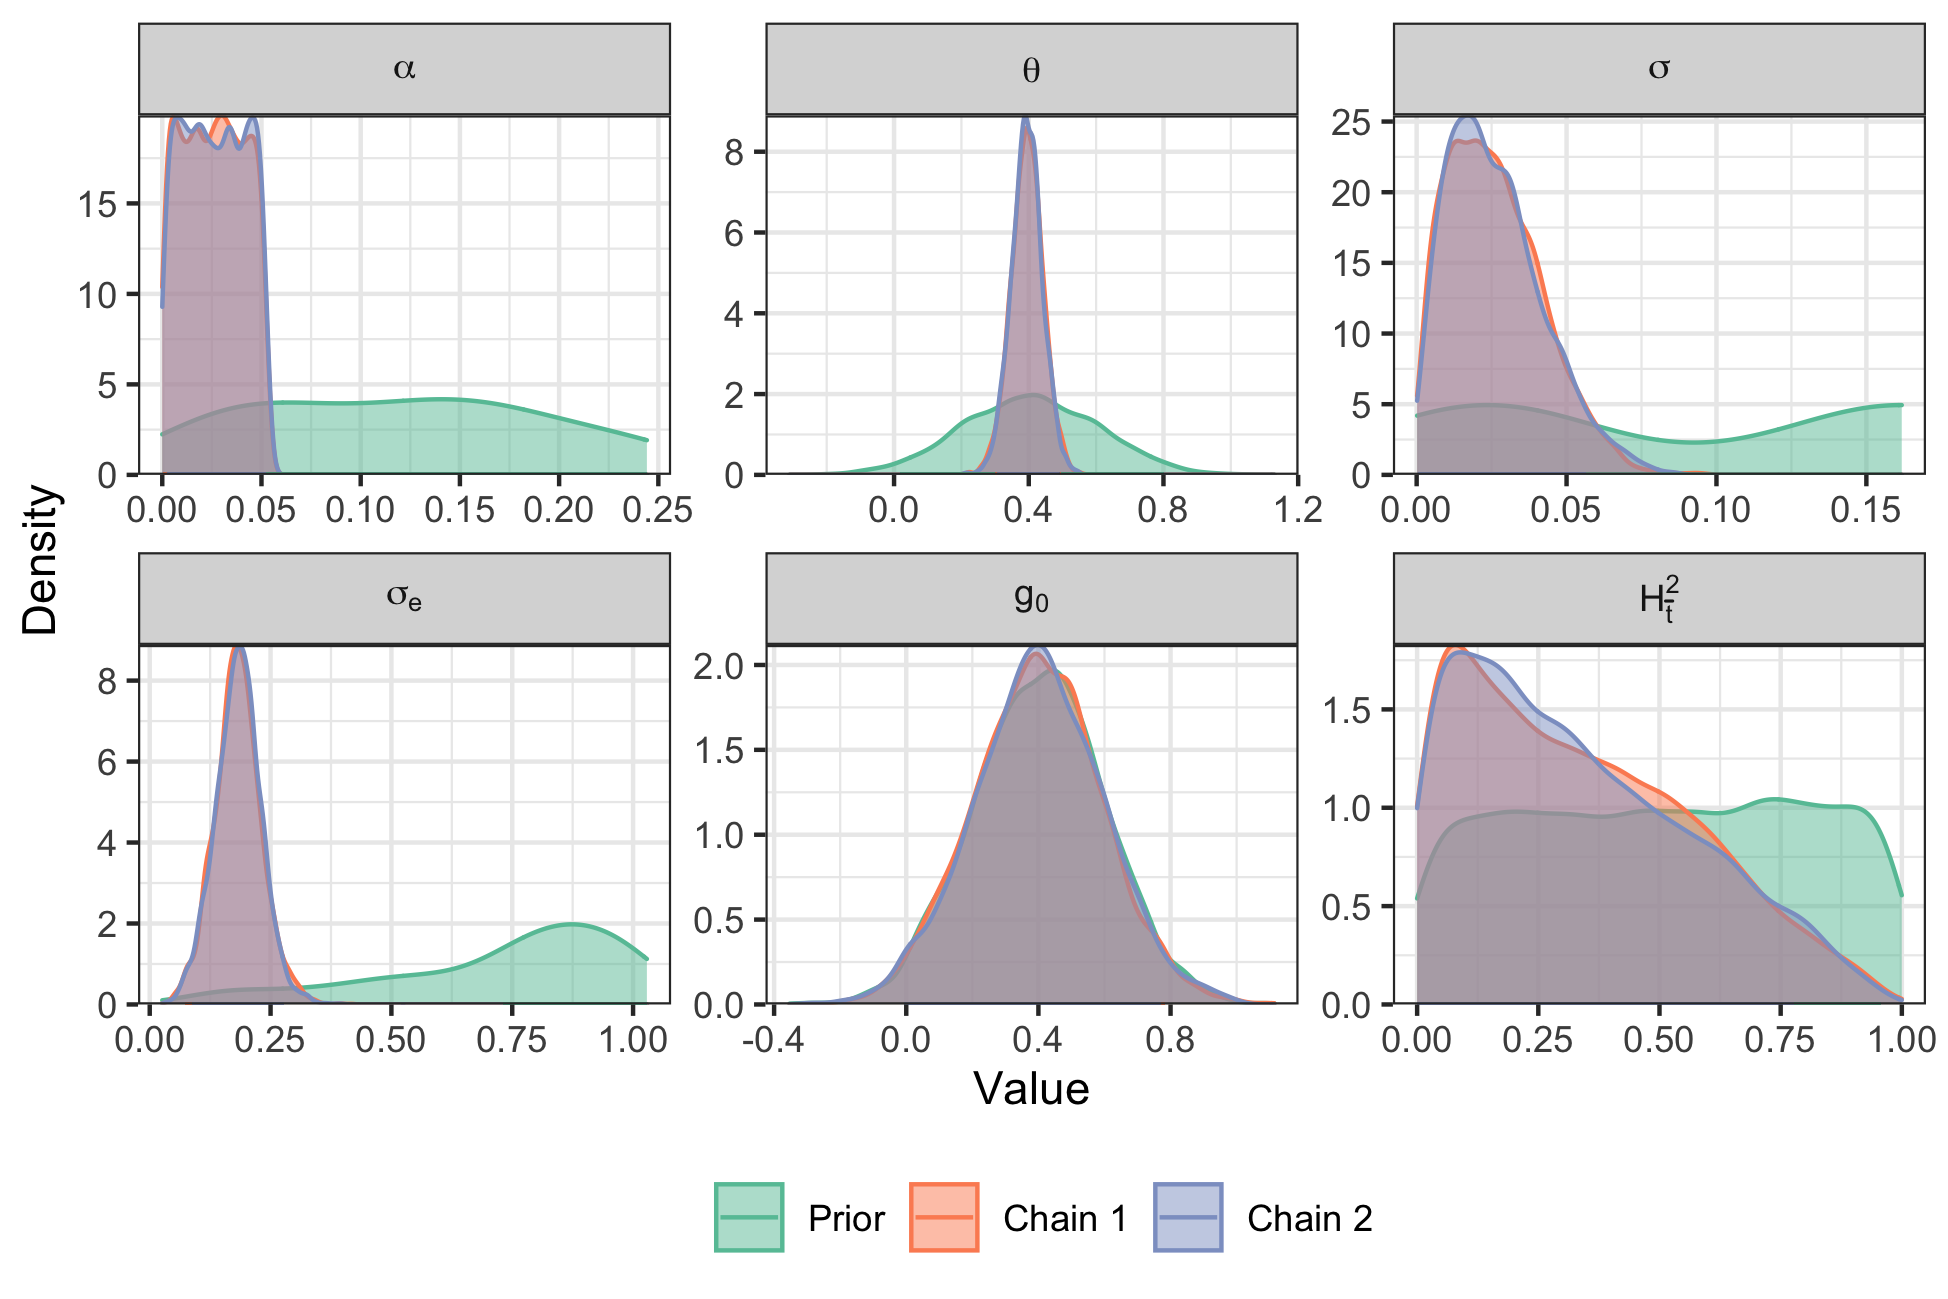
\includegraphics[width=0.7\linewidth]{figures/poumm_parameter_estimates_arboricola.png}
		\caption{\DIFaddFL{Posterior distributions compared to the prior for POUMM parameter estimates based on }\emph{\DIFaddFL{A. thaliana}}\DIFaddFL{-}\emph{\DIFaddFL{X. arboricola}} \DIFaddFL{data. We ran two different MCMC chains to ensure the estimates converged.}}
\label{fig:poumm-parameters-qdr}
\end{figure}

\begin{figure}[H]
\begin{center}
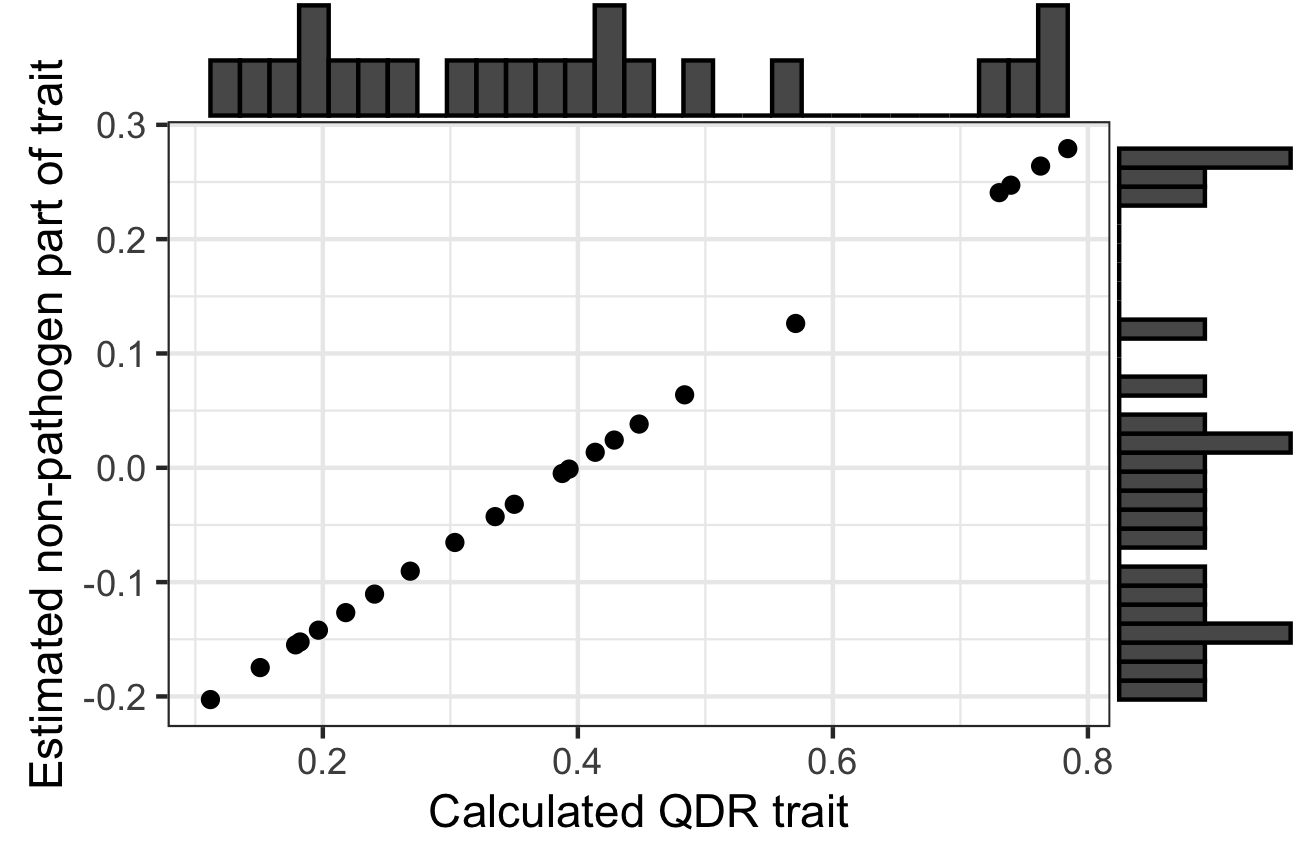
\includegraphics[width = 0.462\linewidth]{figures/trait_values_arboricola.png}
	\caption{\DIFaddFL{A comparison of measured (calculated) mean QDR values across all }\emph{\DIFaddFL{A. thaliana}} \DIFaddFL{accession pairings and replicates  versus our estimated non-pathogen effect on mean QDR for each }\emph{\DIFaddFL{X. arboricola}} \DIFaddFL{pathogen strain. The histograms show the marginal distribution of each value across the strains. The Pearson correlation coefficient is 1.}}
	\label{fig:trait-comparison-qdr}
	\end{center}
\end{figure}

\begin{figure}[H]
\begin{center}
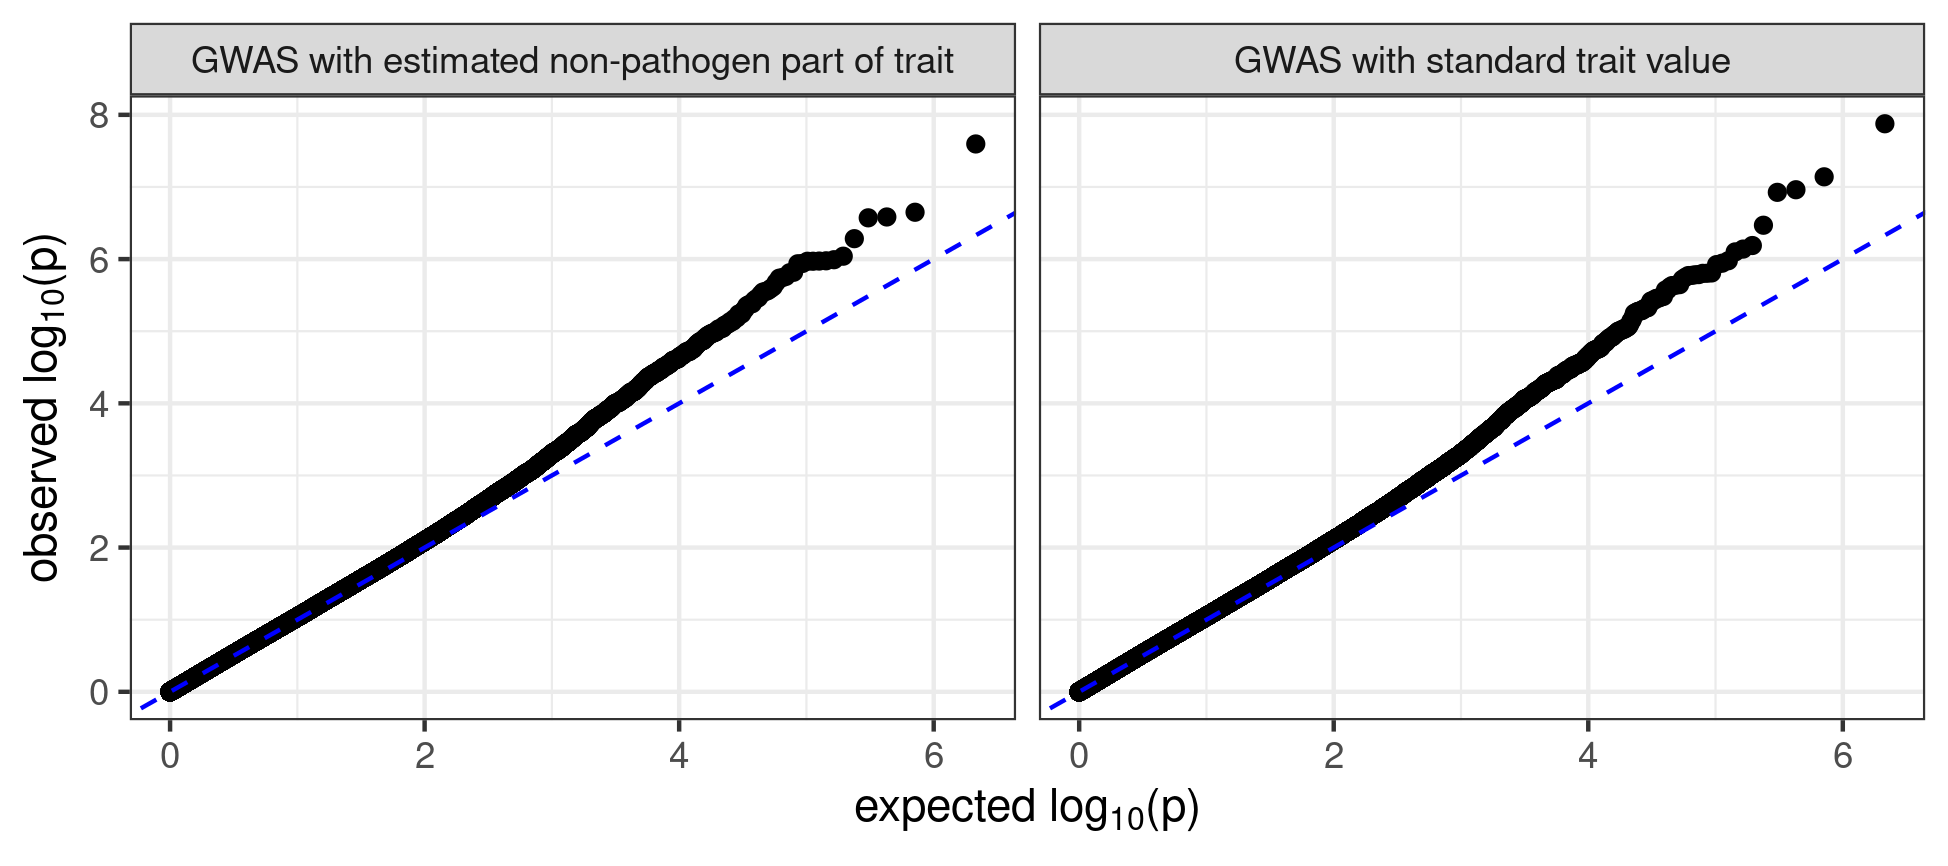
\includegraphics[width = \linewidth]{figures/qq_plots_arabidopsis_xanthomonas.png}
	\caption{\DIFaddFL{Quartile-quartile plots from }\emph{\DIFaddFL{A. thaliana}}\DIFaddFL{-}\emph{\DIFaddFL{X. arboricola}} \DIFaddFL{QDR association tests. The dashed blue line shows the y = x line.}}
	\label{fig:qq-plots-qdr}
	\end{center}
\end{figure}

\begin{figure}[H]
	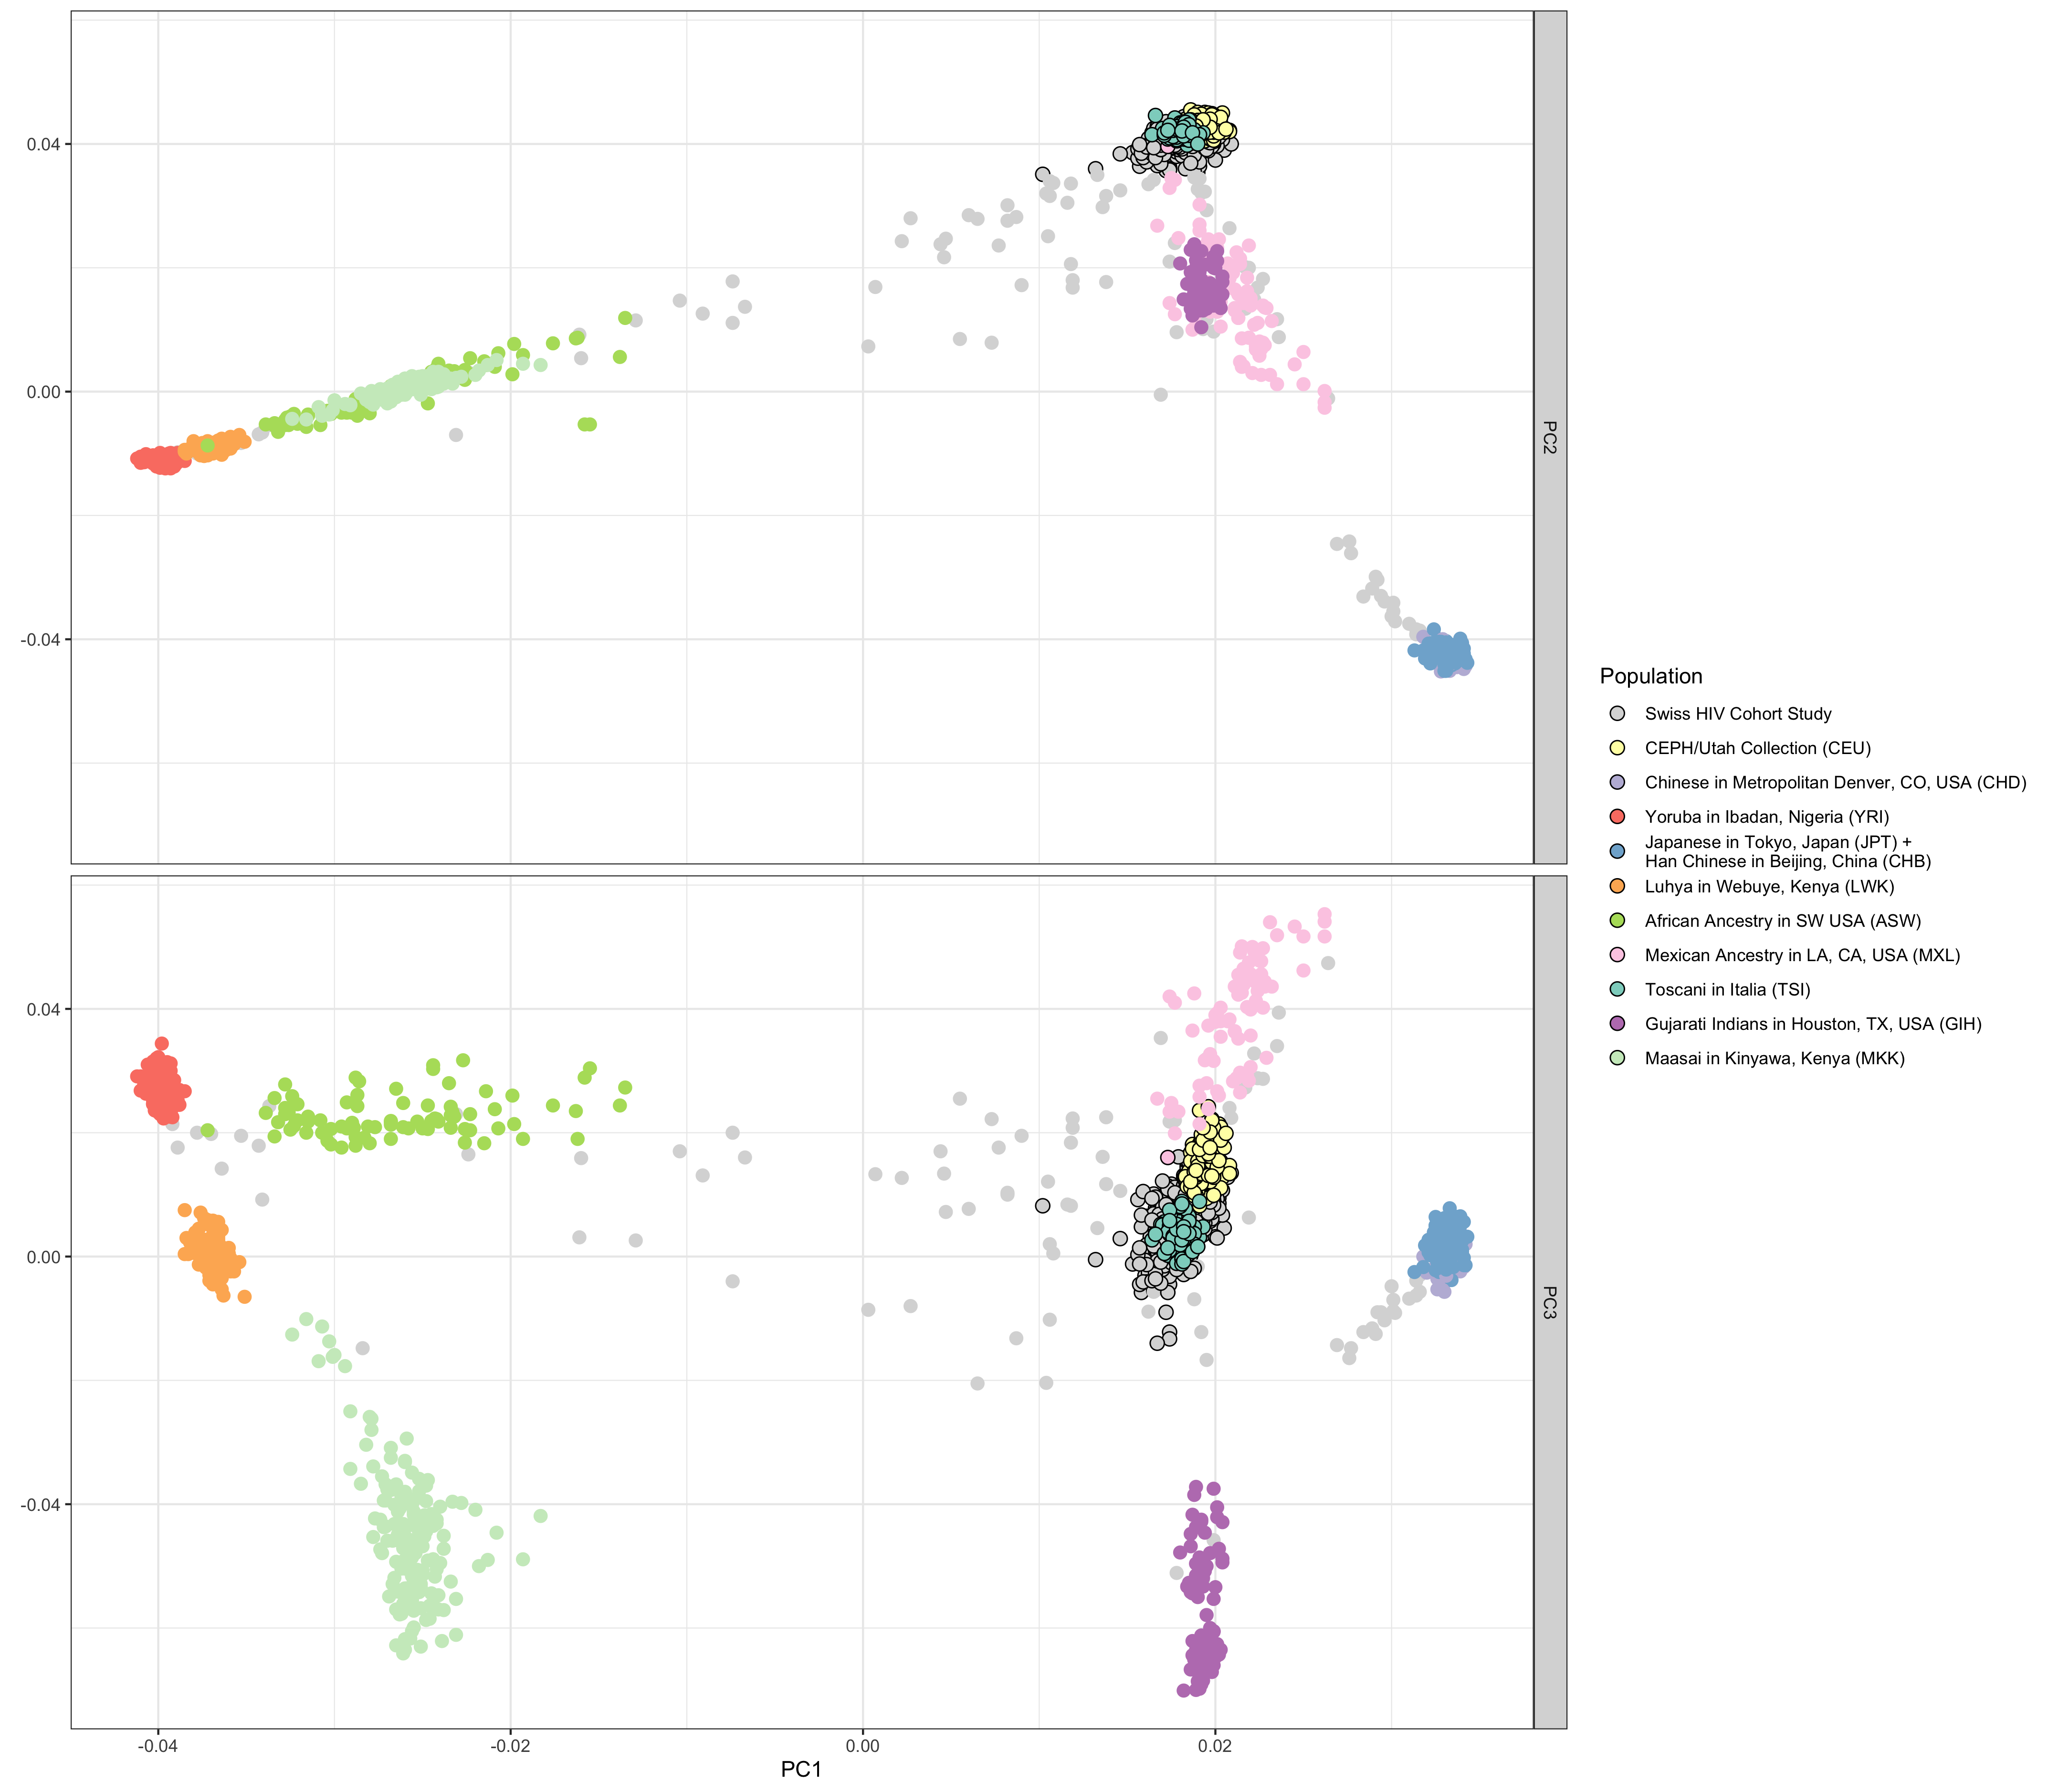
\includegraphics[width=\linewidth]{figures/host_genotype_pca.png}
	\caption{\DIFaddFL{SHCS individuals and HapMap3 individuals plotted along the top three principle components of genetic variation. Points with black borders are within the thresholds used to select individuals of likely European ancestry.}}
	\label{fig:PCA}
\end{figure}

\DIFaddend \end{doublespace}  % don't doublespace tables

\newpage

\begin{table}[H]
	\caption{\DIFdelbeginFL \DIFdelFL{POUMM parameter estimates for spVL based on Swiss data}\DIFdelendFL \DIFaddbeginFL \DIFaddFL{Simulation model parameters}\DIFaddendFL . \DIFdelbeginFL \DIFdelFL{HPD = Highest posterior density}\DIFdelendFL \DIFaddbeginFL \DIFaddFL{For a full graphical model representation of the simulation scheme, including how these parameters are related, see Figure \ref{fig:sim-design}}\DIFaddendFL .}
	\DIFdelbeginFL %DIFDELCMD < \begin{tabularx}{\linewidth}{XXX} \hline 
%DIFDELCMD < 	%%%
\DIFdelFL{Parameter }\DIFdelendFL \DIFaddbeginFL \begin{tabularx}{\linewidth}{p{1.5cm}p{6.5cm}l} \toprule 
		\DIFaddFL{Variable }\DIFaddendFL & \DIFdelbeginFL \DIFdelFL{Posterior mean }\DIFdelendFL \DIFaddbeginFL \DIFaddFL{Expression }\DIFaddendFL & \DIFdelbeginFL \DIFdelFL{95\% HPD }\DIFdelendFL \DIFaddbeginFL \DIFaddFL{Definition }\DIFaddendFL \\ \DIFdelbeginFL %DIFDELCMD < \hline 
%DIFDELCMD < 	%%%
\DIFdelFL{${g_{0}}$ }\DIFdelendFL \DIFaddbeginFL \midrule 
		\DIFaddFL{$\sigma^2_z$ }\DIFaddendFL &  \DIFdelbeginFL \DIFdelFL{4.23 }\DIFdelendFL \DIFaddbeginFL \DIFaddFL{0.73 log copies$^{2}$/mL$^{2}$ }\DIFaddendFL & \DIFdelbeginFL \DIFdelFL{(1.72, 6.71) }\DIFdelendFL \DIFaddbeginFL \DIFaddFL{Total spVL variance }\DIFaddendFL \\ 
		\DIFdelbeginFL \DIFdelFL{$\theta$ }\DIFdelendFL \DIFaddbeginFL \DIFaddFL{$H^2_h$ }\DIFaddendFL & \DIFdelbeginFL \DIFdelFL{4.47 }\DIFdelendFL \DIFaddbeginFL \DIFaddFL{0.25 }\DIFaddendFL & \DIFdelbeginFL \DIFdelFL{(4.37, 4.58) }\DIFdelendFL \DIFaddbeginFL \DIFaddFL{Host heritability of spVL }\DIFaddendFL \\
		\DIFdelbeginFL \DIFdelFL{$\sigma$ }\DIFdelendFL \DIFaddbeginFL \DIFaddFL{$H^2_{\bar{t}}$ }\DIFaddendFL & \DIFdelbeginFL \DIFdelFL{5.25 }\DIFdelendFL \DIFaddbeginFL \DIFaddFL{varied }\DIFaddendFL & \DIFdelbeginFL \DIFdelFL{(2.37, 7.9) }\DIFdelendFL \DIFaddbeginFL \DIFaddFL{Pathogen heritability of spVL at $\bar{t}$ }\DIFaddendFL \\
		\DIFdelbeginFL \DIFdelFL{$\alpha$ }\DIFdelendFL \DIFaddbeginFL \DIFaddFL{$\sigma^2_{h}$ }\DIFaddendFL & \DIFdelbeginFL \DIFdelFL{57.65 }\DIFdelendFL \DIFaddbeginFL \DIFaddFL{$\sigma_{h}^2 = 0.25*\sigma_z^2$ }\DIFaddendFL & \DIFdelbeginFL \DIFdelFL{(19.49, 95.2) }\DIFdelendFL \DIFaddbeginFL \DIFaddFL{Variance in host part of spVL }\DIFaddendFL \\
		\DIFdelbeginFL \DIFdelFL{$\sigma_e$ }\DIFdelendFL \DIFaddbeginFL \DIFaddFL{$\sigma^2_{g}(\bar{t})$ }\DIFaddendFL & \DIFdelbeginFL \DIFdelFL{0.54 }\DIFdelendFL \DIFaddbeginFL \DIFaddFL{$\sigma^2_{g}(\bar{t}) = H^2_{\bar{t}}*\sigma_z^2$ }\DIFaddendFL & \DIFdelbeginFL \DIFdelFL{(0.43, 0.65) }\DIFdelendFL \DIFaddbeginFL \DIFaddFL{Variance in pathogen part of spVL at $\bar{t}$ }\DIFaddendFL \\ 
		\DIFdelbeginFL \DIFdelFL{$H^2_{\bar{t}}$ }\DIFdelendFL \DIFaddbeginFL \DIFaddFL{$\sigma^2_{e}$ }\DIFaddendFL & \DIFdelbeginFL \DIFdelFL{0.45 }\DIFdelendFL \DIFaddbeginFL \DIFaddFL{$\sigma_{e}^2 = \sigma_z^2 - \sigma^2_{g} - \sigma^2_{h}$ }\DIFaddendFL & \DIFdelbeginFL \DIFdelFL{(0.24, 0.67) }\DIFdelendFL \DIFaddbeginFL \DIFaddFL{Variance in environmental part of spVL }\DIFaddendFL \\ 
		\DIFdelbeginFL %DIFDELCMD < \hline
%DIFDELCMD < 	\end{tabularx}
%DIFDELCMD < 	\label{tab:POUMM-parameters-our-estimates}
%DIFDELCMD < \end{table}
%DIFDELCMD < 

%DIFDELCMD < \begin{table}[H]
%DIFDELCMD < %%%
%DIFDELCMD < \caption{%
{%DIFAUXCMD
\DIFdelFL{POUMM parameter estimates for spVL from previous studies.}}
	%DIFAUXCMD
%DIFDELCMD < \begin{tabularx}{\linewidth}{llXXX}
%DIFDELCMD < 	\hline 
%DIFDELCMD < 	%%%
\DIFdelFL{Parameter }\DIFdelendFL \DIFaddbeginFL \DIFaddFL{$\bar{t}$ }\DIFaddendFL & \DIFdelbeginFL \DIFdelFL{Value (Uncertainty) }\DIFdelendFL \DIFaddbeginFL \DIFaddFL{0.14 substitutions site$^{-1}$ yr$^{-1}$ }\DIFaddendFL & \DIFdelbeginFL \DIFdelFL{Reference }%DIFDELCMD < & %%%
\DIFdelFL{Notes }\DIFdelendFL \DIFaddbeginFL \DIFaddFL{Mean root-tip time in pathogen phylogeny }\DIFaddendFL \\ 
		\DIFdelbeginFL %DIFDELCMD < \hline 
%DIFDELCMD < 	%%%
\DIFdelFL{$v_0$ }\DIFdelendFL \DIFaddbeginFL \DIFaddFL{$\bm{g}$ }\DIFaddendFL & \DIFdelbeginFL \DIFdelFL{5.54 (4.04 - 7.25) }\DIFdelendFL \DIFaddbeginFL \DIFaddFL{$\bm{g} \sim Norm(\bm{\mu}_{OU}, \boldsymbol{\Sigma}_{OU})$ }\DIFaddendFL & \DIFdelbeginFL \DIFdelFL{\mbox{%DIFAUXCMD
\citet{Mitov2018} }\hskip0pt%DIFAUXCMD
}%DIFDELCMD < & %%%
\DIFdelFL{8,483 UK HIV cohort individuals , $pol$ tree }\DIFdelendFL \DIFaddbeginFL \DIFaddFL{Pathogen part of spVL for all individuals }\DIFaddendFL \\ 
		$\theta$ & \DIFdelbeginFL \DIFdelFL{4.45 (4.41 - 4.49) }\DIFdelendFL \DIFaddbeginFL \DIFaddFL{4.5 log copies/mL }\DIFaddendFL & \DIFdelbeginFL \DIFdelFL{\mbox{%DIFAUXCMD
\citet{Mitov2018} }\hskip0pt%DIFAUXCMD
}%DIFDELCMD < & %%%
\DIFdelendFL \DIFaddbeginFL \DIFaddFL{Optimal spVL value }\DIFaddendFL \\
		\DIFdelbeginFL \DIFdelFL{$\theta$ }\DIFdelendFL \DIFaddbeginFL \DIFaddFL{$g_{0}$ }\DIFaddendFL & \DIFdelbeginFL \DIFdelFL{4.0 (1.6 - 4.)) }\DIFdelendFL \DIFaddbeginFL \DIFaddFL{4.5 log copies/mL }\DIFaddendFL & \DIFdelbeginFL \DIFdelFL{\mbox{%DIFAUXCMD
\citet{Bertels2018} }\hskip0pt%DIFAUXCMD
}%DIFDELCMD < & %%%
\DIFdelFL{3,036 SHCS individuals, $pol$ tree }\DIFdelendFL \DIFaddbeginFL \DIFaddFL{$g$ at the root of the phylogeny  }\DIFaddendFL \\ 
		\DIFdelbeginFL \DIFdelFL{$\theta$ }%DIFDELCMD < & %%%
\DIFdelFL{4.1 (3.5 - 4.9) }%DIFDELCMD < & %%%
\DIFdelFL{\mbox{%DIFAUXCMD
\citet{Blanquart2017} }\hskip0pt%DIFAUXCMD
}%DIFDELCMD < & %%%
\DIFdelFL{1,581 subtype B individuals from Europe, whole genome tree }%DIFDELCMD < \\
%DIFDELCMD < 	%%%
\DIFdelendFL $\alpha$ & \DIFdelbeginFL \DIFdelFL{28.78 (16.64 - 46.93) }\DIFdelendFL \DIFaddbeginFL \DIFaddFL{varied }\DIFaddendFL & \DIFdelbeginFL \DIFdelFL{\mbox{%DIFAUXCMD
\citet{Mitov2018} }\hskip0pt%DIFAUXCMD
}%DIFDELCMD < & %%%
\DIFdelendFL \DIFaddbeginFL \DIFaddFL{Selection strength of OU process }\DIFaddendFL \\ 
		\DIFdelbeginFL \DIFdelFL{$\alpha$ }%DIFDELCMD < & %%%
\DIFdelFL{32.7 (0.03 - 57.6) }%DIFDELCMD < & %%%
\DIFdelFL{\mbox{%DIFAUXCMD
\citet{Bertels2018} }\hskip0pt%DIFAUXCMD
}%DIFDELCMD < & \\
%DIFDELCMD < 	%%%
\DIFdelFL{$\alpha$ }%DIFDELCMD < & %%%
\DIFdelFL{7.6 (1.2 - 10) }%DIFDELCMD < & %%%
\DIFdelFL{\mbox{%DIFAUXCMD
\citet{Blanquart2017} }\hskip0pt%DIFAUXCMD
}%DIFDELCMD < & %%%
\DIFdelFL{**limited $\alpha$ to $\le$ 10 }%DIFDELCMD < \\
%DIFDELCMD < 	%%%
\DIFdelendFL $\sigma$ & \DIFdelbeginFL \DIFdelFL{2.97 (1.95 - 4.37) }\DIFdelendFL \DIFaddbeginFL \DIFaddFL{$\sigma = \sqrt{\frac{2\alpha\sigma^2_{g}(\bar{t})}{1 - exp(-2\alpha\bar{t})}}$ }\DIFaddendFL & \DIFdelbeginFL \DIFdelFL{\mbox{%DIFAUXCMD
\citet{Mitov2018} }\hskip0pt%DIFAUXCMD
}%DIFDELCMD < & %%%
\DIFdelendFL \DIFaddbeginFL \DIFaddFL{Time-unit standard deviation of OU process }\DIFaddendFL \\ 
		\DIFdelbeginFL \DIFdelFL{$\sigma$ }\DIFdelendFL \DIFaddbeginFL \DIFaddFL{$\Psi$ }\DIFaddendFL & \DIFdelbeginFL \DIFdelFL{1.3 (0.66 -1.87) }\DIFdelendFL \DIFaddbeginFL \DIFaddFL{branch lengths $\sim Exp(\bar{t})$ }\DIFaddendFL & \DIFdelbeginFL \DIFdelFL{\mbox{%DIFAUXCMD
\citet{Blanquart2017} }\hskip0pt%DIFAUXCMD
}%DIFDELCMD < & %%%
\DIFdelendFL \DIFaddbeginFL \DIFaddFL{Pathogen phylogeny }\DIFaddendFL \\ 
		\DIFdelbeginFL \DIFdelFL{$\sigma_e$ }\DIFdelendFL \DIFaddbeginFL \DIFaddFL{$h_i$ }\DIFaddendFL & \DIFdelbeginFL \DIFdelFL{0.77 (0.73, 0.8) }\DIFdelendFL \DIFaddbeginFL \DIFaddFL{$h_i = \delta \sum_{j = 1}^{j = M/2}{G_{ij}} - \delta \sum_{j = M/2}^{j = M}{G_{ij}}$ }\DIFaddendFL & \DIFdelbeginFL \DIFdelFL{\mbox{%DIFAUXCMD
\citet{Mitov2018} }\hskip0pt%DIFAUXCMD
}%DIFDELCMD < & %%%
\DIFdelendFL \DIFaddbeginFL \DIFaddFL{Host part of spVL for individual $i$ }\DIFaddendFL \\ 
		\DIFdelbeginFL \DIFdelFL{$\sigma_e$ }\DIFdelendFL \DIFaddbeginFL \DIFaddFL{$G_{N \times M}$ }\DIFaddendFL & \DIFdelbeginFL \DIFdelFL{0.61 (0.54, 0.65) }\DIFdelendFL \DIFaddbeginFL \makecell{$G_{ij} \sim Binom(2, p)\ \\ \forall i \in {1...N}, \forall j \in {1...M}$} \DIFaddendFL & \DIFdelbeginFL \DIFdelFL{\mbox{%DIFAUXCMD
\citet{Blanquart2017} }\hskip0pt%DIFAUXCMD
}%DIFDELCMD < & %%%
\DIFdelendFL \DIFaddbeginFL \DIFaddFL{Host genotype matrix }\DIFaddendFL \\
		\DIFdelbeginFL %DIFDELCMD < \hline 
%DIFDELCMD < 	\end{tabularx}
%DIFDELCMD < 	\label{tab:POUMMparams-prev-estimated}
%DIFDELCMD < \end{table}
%DIFDELCMD < 

%DIFDELCMD < \begin{table}[H]
%DIFDELCMD < %%%
%DIFDELCMD < \caption{%
{%DIFAUXCMD
\DIFdelFL{Summary statistics for log spVL in previously sampled populations. $\bar{z}$ is average spVL (log copies/mL) and $\sigma^2_z$ is variance in measured spVL ( log $\textrm{copies}^2/\textrm{mL}^2$). Values from }%DIFDELCMD < \protect%%%
\DIFdelFL{\mbox{%DIFAUXCMD
\citep{Blanquart2017, Mitov2018} }\hskip0pt%DIFAUXCMD
are empirical; values from }%DIFDELCMD < \protect%%%
\DIFdelFL{\mbox{%DIFAUXCMD
\citep{Bonhoeffer2015} }\hskip0pt%DIFAUXCMD
were estimated by fitting a normal distribution to the data.}}
	%DIFAUXCMD
%DIFDELCMD < \begin{tabularx}{\linewidth}{XXX} \hline 
%DIFDELCMD < 	%%%
\DIFdelFL{Measurement }\DIFdelendFL \DIFaddbeginFL \DIFaddFL{$p$ }\DIFaddendFL & \DIFdelbeginFL \DIFdelFL{Value }\DIFdelendFL \DIFaddbeginFL \DIFaddFL{$p = \frac{1}{2} - \sqrt{\frac{1}{4} - \frac{H_{h}^2\sigma^2_z}{2\delta^2M}}$ }\DIFaddendFL &  \DIFdelbeginFL \DIFdelFL{Reference }\DIFdelendFL \DIFaddbeginFL \DIFaddFL{Host variant allele frequency }\DIFaddendFL \\ 
		\DIFdelbeginFL %DIFDELCMD < \hline 
%DIFDELCMD < 	%%%
\DIFdelFL{$\bar{z}$ }\DIFdelendFL \DIFaddbeginFL \DIFaddFL{$\delta$ }\DIFaddendFL & \DIFdelbeginFL \DIFdelFL{$\approx$ 4.5 }\DIFdelendFL \DIFaddbeginFL \DIFaddFL{0.2 }\DIFaddendFL & \DIFdelbeginFL \DIFdelFL{\mbox{%DIFAUXCMD
\citet{Mitov2018} }\hskip0pt%DIFAUXCMD
}\DIFdelendFL \DIFaddbeginFL \DIFaddFL{Host variant effect size }\DIFaddendFL \\ 
		\DIFdelbeginFL \DIFdelFL{$\bar{z}$ }\DIFdelendFL \DIFaddbeginFL \DIFaddFL{$M$ }\DIFaddendFL & \DIFdelbeginFL \DIFdelFL{4.4 }\DIFdelendFL \DIFaddbeginFL \DIFaddFL{20 }\DIFaddendFL & \DIFdelbeginFL \DIFdelFL{\mbox{%DIFAUXCMD
\citet{Blanquart2017} }\hskip0pt%DIFAUXCMD
}\DIFdelendFL \DIFaddbeginFL \DIFaddFL{Number of causal host variants }\DIFaddendFL \\ 
		\DIFdelbeginFL \DIFdelFL{$\bar{z}$ }\DIFdelendFL \DIFaddbeginFL \DIFaddFL{$e_i$ }\DIFaddendFL & \DIFdelbeginFL \DIFdelFL{$\approx$ 4.5 }\DIFdelendFL \DIFaddbeginFL \DIFaddFL{$ e_i \sim Norm(0, \sigma^2_{e})$ }\DIFaddendFL & \DIFdelbeginFL \DIFdelFL{\mbox{%DIFAUXCMD
\citet{Bonhoeffer2015} }\hskip0pt%DIFAUXCMD
}\DIFdelendFL \DIFaddbeginFL \DIFaddFL{Environmental part of spVL for individual $i$ }\DIFaddendFL \\ 
		\DIFdelbeginFL \DIFdelFL{$\sigma^2_z$ }\DIFdelendFL \DIFaddbeginFL \DIFaddFL{$N$ }\DIFaddendFL & \DIFdelbeginFL \DIFdelFL{0.73 }\DIFdelendFL \DIFaddbeginFL \DIFaddFL{500 }\DIFaddendFL & \DIFdelbeginFL \DIFdelFL{\mbox{%DIFAUXCMD
\citet{Mitov2018} }\hskip0pt%DIFAUXCMD
}\DIFdelendFL \DIFaddbeginFL \DIFaddFL{Number of simulated samples }\DIFaddendFL \\ \DIFdelbeginFL \DIFdelFL{$\sigma^2_z$ }%DIFDELCMD < &  %%%
\DIFdelFL{0.50 }%DIFDELCMD < & %%%
\DIFdelFL{\mbox{%DIFAUXCMD
\citet{Blanquart2017} }\hskip0pt%DIFAUXCMD
}%DIFDELCMD < \\
%DIFDELCMD < 	%%%
\DIFdelFL{$\sigma^2_z$ }%DIFDELCMD < & %%%
\DIFdelFL{$\approx$ 0.5 }%DIFDELCMD < & %%%
\DIFdelFL{\mbox{%DIFAUXCMD
\citet{Bonhoeffer2015} }\hskip0pt%DIFAUXCMD
}%DIFDELCMD < \\ \hline 
%DIFDELCMD < 	%%%
\DIFdelendFL \DIFaddbeginFL \bottomrule 
	\DIFaddendFL \end{tabularx}
	\DIFdelbeginFL %DIFDELCMD < \label{tab:spVLmeasurements}
%DIFDELCMD < %%%
\DIFdelendFL \DIFaddbeginFL \label{tab:sim-params}
\DIFaddendFL \end{table}
%DIF < \todo{I guessed at bar(z) from figure in Mitov2018, search supplement for exact}

\begin{table}[H]
\caption{\DIFdelbeginFL \DIFdelFL{Number of samples }\DIFdelendFL \DIFaddbeginFL \DIFaddFL{POUMM parameter estimates }\DIFaddendFL for \DIFdelbeginFL \DIFdelFL{GWAS after sequential filtering steps}\DIFdelendFL \DIFaddbeginFL \DIFaddFL{spVL based on SHCS data}\DIFaddendFL . \DIFaddbeginFL \DIFaddFL{HPD = Highest posterior density.}\DIFaddendFL }
	\DIFdelbeginFL %DIFDELCMD < \begin{tabularx}{\linewidth}{XX}
%DIFDELCMD <     %%%
\DIFdelendFL \DIFaddbeginFL \begin{tabularx}{\linewidth}{XXX} \DIFaddendFL \hline 
	\DIFdelbeginFL \DIFdelFL{Sample filter }\DIFdelendFL \DIFaddbeginFL \DIFaddFL{Parameter }\DIFaddendFL & \DIFdelbeginFL \DIFdelFL{Number of samples remaining }\DIFdelendFL \DIFaddbeginFL \DIFaddFL{Posterior mean }& \DIFaddFL{95\% HPD }\DIFaddendFL \\ \hline 
	\DIFdelbeginFL \DIFdelFL{Subtype B pol sequences }\DIFdelendFL \DIFaddbeginFL \DIFaddFL{${g_{0}}$ }\DIFaddendFL & \DIFdelbeginFL \DIFdelFL{1516 }%DIFDELCMD < \\
%DIFDELCMD <     %%%
\DIFdelFL{With paired spVL measurement }\DIFdelendFL \DIFaddbeginFL \DIFaddFL{4.23 }\DIFaddendFL & \DIFdelbeginFL \DIFdelFL{1516 }\DIFdelendFL \DIFaddbeginFL \DIFaddFL{(1.72, 6.71) }\DIFaddendFL \\
	\DIFdelbeginFL \DIFdelFL{$>$ 750 characters in sequence }\DIFdelendFL \DIFaddbeginFL \DIFaddFL{$\theta$ }\DIFaddendFL & \DIFdelbeginFL \DIFdelFL{1493 }%DIFDELCMD < \\
%DIFDELCMD <     %%%
\DIFdelFL{Individual is of European ancestry }\DIFdelendFL \DIFaddbeginFL \DIFaddFL{4.47 }\DIFaddendFL & \DIFdelbeginFL \DIFdelFL{1396 }\DIFdelendFL \DIFaddbeginFL \DIFaddFL{(4.37, 4.58) }\DIFaddendFL \\
	\DIFdelbeginFL \DIFdelFL{Kinship coefficient $>$ 0.09375 }\DIFdelendFL \DIFaddbeginFL \DIFaddFL{$\sigma$ }\DIFaddendFL & \DIFdelbeginFL \DIFdelFL{1392 }%DIFDELCMD < \\ 
%DIFDELCMD <     \hline
%DIFDELCMD <     \end{tabularx}
%DIFDELCMD <     \label{tab:sample-filtering}
%DIFDELCMD < \end{table}
%DIFDELCMD < 

%DIFDELCMD < \begin{table}[H]
%DIFDELCMD < %%%
%DIFDELCMD < \caption{%
{%DIFAUXCMD
\DIFdelFL{Number of variants for GWAS after sequential filtering steps.}}
	%DIFAUXCMD
%DIFDELCMD < \begin{tabularx}{\linewidth}{XX}
%DIFDELCMD < 	\hline
%DIFDELCMD < 	%%%
\DIFdelFL{Variant filter }\DIFdelendFL \DIFaddbeginFL \DIFaddFL{5.25 }\DIFaddendFL & \DIFdelbeginFL \DIFdelFL{Number of variants remaining }\DIFdelendFL \DIFaddbeginFL \DIFaddFL{(2.37, 7.9) }\DIFaddendFL \\
	\DIFdelbeginFL %DIFDELCMD < \hline 
%DIFDELCMD < 	%%%
\DIFdelFL{Raw data }\DIFdelendFL \DIFaddbeginFL \DIFaddFL{$\alpha$ }\DIFaddendFL & \DIFdelbeginFL \DIFdelFL{76979521 }%DIFDELCMD < \\
%DIFDELCMD < 	%%%
\DIFdelFL{Missing genotype rate $>$ 0.05 }\DIFdelendFL \DIFaddbeginFL \DIFaddFL{57.65 }\DIFaddendFL & \DIFdelbeginFL \DIFdelFL{11590002 }\DIFdelendFL \DIFaddbeginFL \DIFaddFL{(19.49, 95.2) }\DIFaddendFL \\
	\DIFdelbeginFL \DIFdelFL{Hardy-Weinburg exact test p-value $< 5 \times 10^{-5}$ }\DIFdelendFL \DIFaddbeginFL \DIFaddFL{$\sigma_\epsilon$ }\DIFaddendFL & \DIFdelbeginFL \DIFdelFL{11589246 }\DIFdelendFL \DIFaddbeginFL \DIFaddFL{0.54 }& \DIFaddFL{(0.43, 0.65) }\DIFaddendFL \\ 
	\DIFdelbeginFL \DIFdelFL{Minor allele frequency $<$ 0.01 }\DIFdelendFL \DIFaddbeginFL \DIFaddFL{$H^2_{\bar{t}}$ }\DIFaddendFL & \DIFdelbeginFL \DIFdelFL{6228626 }\DIFdelendFL \DIFaddbeginFL \DIFaddFL{0.45 }& \DIFaddFL{(0.24, 0.67) }\DIFaddendFL \\ \hline
	\end{tabularx}
	\DIFdelbeginFL %DIFDELCMD < \label{tab:variant-filtering}
%DIFDELCMD < %%%
\DIFdelendFL \DIFaddbeginFL \label{tab:POUMM-parameters-our-estimates}
\DIFaddendFL \end{table}

% latex table generated in R 4.1.1 by xtable 1.8-4 package
% Sat Oct 30 10:31:16 2021
\begin{table}[ht]
\caption{Effect size and p-values from \DIFdelbeginFL \DIFdelFL{top-associated }\DIFdelendFL \DIFaddbeginFL \DIFaddFL{the top most strongly associated }\DIFaddendFL variants in the $\emph{CCR5}$ and MCR regions from \DIFaddbeginFL \DIFaddFL{each of }\DIFaddendFL the two GWAS performed in our study. ``Standard'' means the GWAS with standard spVL trait values and ``Corrected'' means the GWAS with the estimated non-pathogen part of the trait. \DIFaddbeginFL \DIFaddFL{Entries above the dividing line are the top-associated variants from the ``Standard'' GWAS and entries below the dividing line are the top-associated variants from the ``Corrected'' GWAS. Many entries overlap between the two.}\DIFaddendFL }
\begin{tabularx}{\linewidth}{XXXXXXX}
  \hline
    Region & Position & Variant & Standard effect size & Standard p-value & Corrected effect size & Corrected p-value \\ 
  \hline
    $\emph{CCR5}$ & 46531144 & rs9845968 & -0.16 & $5.6 \times 10^{-9}$ & -0.083 & $1.2 \times 10^{-7}$ \\ 
    $\emph{CCR5}$ & 46537849 & rs867620 & -0.16 & $3.2 \times 10^{-9}$ & -0.085 & $6 \times 10^{-8}$ \\ 
    $\emph{CCR5}$ & 46539864 & rs11130092 & -0.16 & $1.1 \times 10^{-9}$ & -0.087 & $2.6 \times 10^{-8}$ \\ 
    $\emph{CCR5}$ & 46540932 & rs10865942 & -0.16 & $8.4 \times 10^{-9}$ & -0.081 & $4 \times 10^{-7}$ \\ 
    $\emph{CCR5}$ & 46541147 & rs7430431 & -0.17 & $9.2 \times 10^{-10}$ & -0.088 & $2.3 \times 10^{-8}$ \\ 
    MHC & 31274380 & rs9264942 & -0.21 & $4.5 \times 10^{-13}$ & -0.12 & $3.7 \times 10^{-13}$ \\ 
    MHC & 31321919 & rs1055821 & -0.33 & $9.4 \times 10^{-13}$ & -0.19 & $1.4 \times 10^{-12}$ \\ 
    MHC & 31380034 & rs112243036 & -0.32 & $9.9 \times 10^{-16}$ & -0.17 & $3.7 \times 10^{-14}$ \\ 
    MHC & 31391401 & rs4418214 & -0.34 & $2.4 \times 10^{-14}$ & -0.18 & $2.5 \times 10^{-12}$ \\ 
    MHC & 31400137 & rs138130755 & -0.46 & $1 \times 10^{-12}$ & -0.26 & $2.6 \times 10^{-12}$ \\ 
    MHC & 31400705 & rs138117378 & -0.46 & $1 \times 10^{-12}$ & -0.26 & $2.6 \times 10^{-12}$ \\ 
    MHC & 31402358 & rs148792134 & -0.46 & $1 \times 10^{-12}$ & -0.26 & $2.6 \times 10^{-12}$ \\ 
    MHC & 31409677 & rs140991764 & -0.46 & $1 \times 10^{-12}$ & -0.26 & $2.6 \times 10^{-12}$ \\ 
    \DIFaddbeginFL \hline
    \DIFaddendFL $\emph{CCR5}$ & 46531144 & rs9845968 & -0.16 & $5.6 \times 10^{-9}$ & -0.083 & $1.2 \times 10^{-7}$ \\ 
    $\emph{CCR5}$ & 46537849 & rs867620 & -0.16 & $3.2 \times 10^{-9}$ & -0.085 & $6 \times 10^{-8}$ \\ 
    $\emph{CCR5}$ & 46539864 & rs11130092 & -0.16 & $1.1 \times 10^{-9}$ & -0.087 & $2.6 \times 10^{-8}$ \\ 
    $\emph{CCR5}$ & 46541147 & rs7430431 & -0.17 & $9.2 \times 10^{-10}$ & -0.088 & $2.3 \times 10^{-8}$ \\ 
    $\emph{CCR5}$ & 46556835 & rs6808142 & 0.15 & $8.3 \times 10^{-8}$ & 0.082 & $3.3 \times 10^{-7}$ \\ 
    MHC & 31274380 & rs9264942 & -0.21 & $4.5 \times 10^{-13}$ & -0.12 & $3.7 \times 10^{-13}$ \\ 
    MHC & 31321919 & rs1055821 & -0.33 & $9.4 \times 10^{-13}$ & -0.19 & $1.4 \times 10^{-12}$ \\ 
    MHC & 31367874 & rs111281598 & -0.37 & $1.5 \times 10^{-12}$ & -0.22 & $2.1 \times 10^{-12}$ \\ 
    MHC & 31376266 & rs73400361 & -0.37 & $1.4 \times 10^{-12}$ & -0.22 & $2.1 \times 10^{-12}$ \\ 
    MHC & 31380034 & rs112243036 & -0.32 & $9.9 \times 10^{-16}$ & -0.17 & $3.7 \times 10^{-14}$ \\ 
   \hline
\end{tabularx}
\label{tab:gwas-top-associations}
\DIFaddbeginFL \end{table}

\begin{table}[H]
\centering
\caption{\DIFaddFL{Results comparison using three different approximate maximum likelihood HIV-1 phylogenies (see Materials and Methods).}}
\begin{tabularx}{\linewidth}{p{1.8cm}p{2cm}p{1.8cm}p{2cm}p{1.8cm}p{2cm}p{1.8cm}} %DIF >  {lrrrrrr} {llclcccc}
\hline
& \multicolumn{2}{l}{\makecell{Estimated\\non-pathogen\\part of trait\\main tree}} & \multicolumn{2}{l}{\makecell{Estimated\\non-pathogen\\part of trait\\tree 2}} & \multicolumn{2}{l}{\makecell{Estimated\\non-pathogen\\part of trait\\tree 3}} \\ 
  \hline
 \DIFaddFL{Variant }& \DIFaddFL{Effect size }& \DIFaddFL{p-value }& \DIFaddFL{Effect size }& \DIFaddFL{p-value }& \DIFaddFL{Effect size }& \DIFaddFL{p-value }\\
  \hline
    \DIFaddFL{rs59440261 }& \DIFaddFL{-0.22 }& \DIFaddFL{$2.6 \times 10^{-10}$ }& \DIFaddFL{-0.22 }& \DIFaddFL{$1.5 \times 10^{-10}$ }& \DIFaddFL{-0.24 }& \DIFaddFL{$1.4 \times 10^{-10}$ }\\ 
    \DIFaddFL{rs1015164 }& \DIFaddFL{0.078 }& \DIFaddFL{$8.5 \times 10^{-6}$ }& \DIFaddFL{0.076 }& \DIFaddFL{$9.5 \times 10^{-6}$ }& \DIFaddFL{0.083 }& \DIFaddFL{$9 \times 10^{-6}$ }\\ 
   \hline
\end{tabularx}
\label{tab:comp-gwas-mclaren-snps-alt-trees}
\end{table}

\begin{table}[H]
\caption{\DIFaddFL{POUMM parameter estimates for QDR based on }\emph{\DIFaddFL{A. thaliana}}\DIFaddFL{-}\emph{\DIFaddFL{X. arboricola}} \DIFaddFL{data. HPD = Highest posterior density.}}
	\begin{tabularx}{\linewidth}{XXX} \hline 
	\DIFaddFL{Parameter }& \DIFaddFL{Posterior mean }& \DIFaddFL{95\% HPD }\\ \hline 
	\DIFaddFL{${g_{0}}$ }& \DIFaddFL{0.40 }& \DIFaddFL{(0.01, 0.78) }\\
	\DIFaddFL{$\theta$ }& \DIFaddFL{0.39 }& \DIFaddFL{(0.30, 0.49) }\\
	\DIFaddFL{$\sigma$ }& \DIFaddFL{0.03 }& \DIFaddFL{(0.0, 0.06) }\\
	\DIFaddFL{$\alpha$ }& \DIFaddFL{0.03 }& \DIFaddFL{(0.0, 0.05) }\\
	\DIFaddFL{$\sigma_\epsilon$ }& \DIFaddFL{0.18 }& \DIFaddFL{(0.08, 0.27) }\\ 
	\DIFaddFL{$H^2_{\bar{t}}$ }& \DIFaddFL{0.33 }& \DIFaddFL{(0.0, 0.77) }\\ \hline
	\end{tabularx}
	\label{tab:POUMM-parameters-our-estimates-qdr}
\end{table}

\begin{table}[H]
\caption{\DIFaddFL{Summary statistics for log spVL in previously sampled populations. $\bar{z}$ is average spVL (log copies/mL) and $\sigma^2_z$ is variance in measured spVL ( log $\textrm{copies}^2/\textrm{mL}^2$). Values from }\protect\DIFaddFL{\mbox{%DIFAUXCMD
\citep{Blanquart2017, Mitov2018} }\hskip0pt%DIFAUXCMD
are empirical; values from }\protect\DIFaddFL{\mbox{%DIFAUXCMD
\citep{Bonhoeffer2015} }\hskip0pt%DIFAUXCMD
were estimated by fitting a normal distribution to the data.}}
	\begin{tabularx}{\linewidth}{XXX} \hline 
	\DIFaddFL{Measurement }& \DIFaddFL{Value }& \DIFaddFL{Reference }\\ \hline 
	\DIFaddFL{$\bar{z}$ }& \DIFaddFL{$\approx$ 4.5 }& \DIFaddFL{\mbox{%DIFAUXCMD
\citet{Mitov2018} }\hskip0pt%DIFAUXCMD
}\\
	\DIFaddFL{$\bar{z}$ }&  \DIFaddFL{4.4 }& \DIFaddFL{\mbox{%DIFAUXCMD
\citet{Blanquart2017} }\hskip0pt%DIFAUXCMD
}\\
	\DIFaddFL{$\bar{z}$ }& \DIFaddFL{$\approx$ 4.5 }& \DIFaddFL{\mbox{%DIFAUXCMD
\citet{Bonhoeffer2015} }\hskip0pt%DIFAUXCMD
}\\
	\DIFaddFL{$\sigma^2_z$ }&  \DIFaddFL{0.73 }&  \DIFaddFL{\mbox{%DIFAUXCMD
\citet{Mitov2018} }\hskip0pt%DIFAUXCMD
}\\
	\DIFaddFL{$\sigma^2_z$ }&  \DIFaddFL{0.50 }& \DIFaddFL{\mbox{%DIFAUXCMD
\citet{Blanquart2017} }\hskip0pt%DIFAUXCMD
}\\
	\DIFaddFL{$\sigma^2_z$ }& \DIFaddFL{$\approx$ 0.5 }& \DIFaddFL{\mbox{%DIFAUXCMD
\citet{Bonhoeffer2015} }\hskip0pt%DIFAUXCMD
}\\ \hline 
	\end{tabularx}
	\label{tab:spVLmeasurements}
\end{table}
%DIF > \todo{I guessed at bar(z) from figure in Mitov2018, search supplement for exact}

\begin{table}[H]
\caption{\DIFaddFL{POUMM parameter estimates for spVL from previous studies.}}
	\begin{tabularx}{\linewidth}{llXXX}
	\hline 
	\DIFaddFL{Parameter }& \DIFaddFL{Value (Uncertainty) }& \DIFaddFL{Reference }& \DIFaddFL{Notes }\\
	\hline 
	\DIFaddFL{$g_0$ }& \DIFaddFL{5.54 (4.04 - 7.25) }& \DIFaddFL{\mbox{%DIFAUXCMD
\citet{Mitov2018} }\hskip0pt%DIFAUXCMD
}& \DIFaddFL{8,483 UK HIV cohort individuals, $pol$ tree }\\
	\DIFaddFL{$\theta$ }& \DIFaddFL{4.45 (4.41 - 4.49) }& \DIFaddFL{\mbox{%DIFAUXCMD
\citet{Mitov2018} }\hskip0pt%DIFAUXCMD
}& \\
	\DIFaddFL{$\theta$ }&  \DIFaddFL{4.0 (1.6 - 4.)) }& \DIFaddFL{\mbox{%DIFAUXCMD
\citet{Bertels2018} }\hskip0pt%DIFAUXCMD
}& \DIFaddFL{3,036 SHCS individuals, $pol$ tree }\\
	\DIFaddFL{$\theta$ }& \DIFaddFL{4.1 (3.5 - 4.9) }& \DIFaddFL{\mbox{%DIFAUXCMD
\citet{Blanquart2017} }\hskip0pt%DIFAUXCMD
}& \DIFaddFL{1,581 subtype B individuals from Europe, whole genome tree }\\
	\DIFaddFL{$\alpha$ }& \DIFaddFL{28.78 (16.64 - 46.93) }& \DIFaddFL{\mbox{%DIFAUXCMD
\citet{Mitov2018} }\hskip0pt%DIFAUXCMD
}& \\
	\DIFaddFL{$\alpha$ }& \DIFaddFL{32.7 (0.03 - 57.6) }& \DIFaddFL{\mbox{%DIFAUXCMD
\citet{Bertels2018} }\hskip0pt%DIFAUXCMD
}& \\
	\DIFaddFL{$\alpha$ }& \DIFaddFL{7.6 (1.2 - 10) }& \DIFaddFL{\mbox{%DIFAUXCMD
\citet{Blanquart2017} }\hskip0pt%DIFAUXCMD
}& \DIFaddFL{**limited $\alpha$ to $\le$ 10 }\\
	\DIFaddFL{$\sigma$ }& \DIFaddFL{2.97 (1.95 - 4.37) }& \DIFaddFL{\mbox{%DIFAUXCMD
\citet{Mitov2018} }\hskip0pt%DIFAUXCMD
}& \\
	\DIFaddFL{$\sigma$ }& \DIFaddFL{1.3 (0.66 -1.87) }&  \DIFaddFL{\mbox{%DIFAUXCMD
\citet{Blanquart2017} }\hskip0pt%DIFAUXCMD
}& \\
	\DIFaddFL{$\sigma_e$ }& \DIFaddFL{0.77 (0.73, 0.8) }& \DIFaddFL{\mbox{%DIFAUXCMD
\citet{Mitov2018} }\hskip0pt%DIFAUXCMD
}& \\
	\DIFaddFL{$\sigma_e$ }& \DIFaddFL{0.61 (0.54, 0.65) }&  \DIFaddFL{\mbox{%DIFAUXCMD
\citet{Blanquart2017} }\hskip0pt%DIFAUXCMD
}& \\
	\hline 
	\end{tabularx}
	\label{tab:POUMMparams-prev-estimated}
\end{table}

\begin{table}[H]
\caption{\DIFaddFL{Number of samples for HIV-1 spVL GWAS after sequential filtering steps.}}
    \begin{tabularx}{\linewidth}{XX}
    \hline
    \DIFaddFL{Sample filter }& \DIFaddFL{Number of samples remaining }\\
    \hline
    \DIFaddFL{Subtype B pol sequences }& \DIFaddFL{1516 }\\
    \DIFaddFL{With paired spVL measurement }& \DIFaddFL{1516 }\\
    \DIFaddFL{$>$ 750 characters in sequence }& \DIFaddFL{1493 }\\
    \DIFaddFL{Individual is of European ancestry }& \DIFaddFL{1396 }\\
    \DIFaddFL{Kinship coefficient $>$ 0.09375 }& \DIFaddFL{1392 }\\ 
    \hline
    \end{tabularx}
    \label{tab:sample-filtering}
\end{table}

\begin{table}[H]
\caption{\DIFaddFL{Number of variants for HIV-1 spVL GWAS after sequential filtering steps.}}
	\begin{tabularx}{\linewidth}{XX}
	\hline
	\DIFaddFL{Variant filter }& \DIFaddFL{Number of variants remaining }\\
	\hline 
	\DIFaddFL{Raw data }& \DIFaddFL{76979521 }\\
	\DIFaddFL{Missing genotype rate $>$ 0.05 }& \DIFaddFL{11590002 }\\
	\DIFaddFL{Hardy-Weinburg exact test p-value $< 5 \times 10^{-5}$ }& \DIFaddFL{11589246 }\\
	\DIFaddFL{Minor allele frequency $<$ 0.01 }& \DIFaddFL{6228626 }\\ \hline			
	\end{tabularx}
	\label{tab:variant-filtering}
\end{table}

\begin{table}[H]
\caption{\DIFaddFL{Number of variants for }\emph{\DIFaddFL{A. thaliana}} \DIFaddFL{QDR GWAS after sequential filtering steps. The last entry lists variants without GWAS p-values because PLINK assessed the correlation between predictor variables (the variant and the top 5 principle components of host genetic variation are predictors) to be too strong. This did not occur in the HIV-1 spVL GWAS.}}
	\begin{tabularx}{\linewidth}{XX}
	\hline
	\DIFaddFL{Variant filter }& \DIFaddFL{Number of variants remaining }\\
	\hline 
	\DIFaddFL{Raw data }& \DIFaddFL{12883854 }\\
	\DIFaddFL{Bi-allelic variants }& \DIFaddFL{11769920 }\\
	\DIFaddFL{Minor allele frequency $<$ 0.1 }& \DIFaddFL{1743952 }\\
	\DIFaddFL{NA p-value (too-high covariate correlation) }& \DIFaddFL{1070541 }\\ \hline			
	\end{tabularx}
	\label{tab:variant-filtering-qdr}
\DIFaddendFL \end{table}

\stopsection
\end{document}